% === Cours de Java
% === Fichier principal
\usepackage{java}

\title{Le Langage Java}
\subtitle{1�re ann\'ee}
\institute[HEB-ESI]{Haute �cole de Bruxelles --- �cole Sup�rieure d'Informatique}    
\date[2011 --- 2012]{Ann�e acad�mique 2011 / 2012}
\author[]{ \small
  M.~Bastreghi \and J.~Beleho \and P.~Bettens \and M.~Codutti 
  \and A.~Hallal \and C.~Leruste \and D.~Nabet \and N.~Pettiaux \and A.~Rousseau
}

\begin{document}
\begin{frame}
\titlepage
\end{frame}

% ===== Inclusion des diffrents chapitres =====

\setbeamertemplate{section in toc}[square] 
\setbeamerfont{section in toc}{size=\small}

\begin{frame}{Liste des le\c cons --- Quadrimestre I}
\vspace{-20pt}
\begin{columns}[T]
  \begin{column}{0.55\textwidth}
  \tableofcontents[hideallsubsections,sections={1}]
  \vspace{-15pt}
  \tableofcontents[hideallsubsections,sections={2}]
  \vspace{-15pt}
  \tableofcontents[hideallsubsections,sections={3}]
  \vspace{-15pt}
  \tableofcontents[hideallsubsections,sections={4}]
  \vspace{-15pt}
  \tableofcontents[hideallsubsections,sections={5}]
  \vspace{-15pt}
  \tableofcontents[hideallsubsections,sections={6}]
  \vspace{-15pt}
  \tableofcontents[hideallsubsections,sections={7}]
  \vspace{-15pt}
  \tableofcontents[hideallsubsections,sections={8}]
  \vspace{-15pt}
  \tableofcontents[hideallsubsections,sections={9}]
  \vspace{-15pt}
  \tableofcontents[hideallsubsections,sections={10}]
  \vspace{-15pt}
  \tableofcontents[hideallsubsections,sections={11}]
  \vspace{-15pt}
  \tableofcontents[hideallsubsections,sections={12}]
  \end{column}
  \begin{column}{0.45\textwidth}
  \tableofcontents[hideallsubsections,sections={13}]
  \vspace{-15pt}
  \tableofcontents[hideallsubsections,sections={14}]
  \vspace{-15pt}
  \tableofcontents[hideallsubsections,sections={15}]
  \vspace{-15pt}
  \tableofcontents[hideallsubsections,sections={16}]
  \vspace{-15pt}
  \tableofcontents[hideallsubsections,sections={17}]
  \vspace{-15pt}
  \tableofcontents[hideallsubsections,sections={18}]
  \vspace{-15pt}
  \tableofcontents[hideallsubsections,sections={19}]
  \vspace{-15pt}
  \tableofcontents[hideallsubsections,sections={20}]
  \vspace{-15pt}
  \tableofcontents[hideallsubsections,sections={21}]
  \vspace{-15pt}
  \tableofcontents[hideallsubsections,sections={22}]
  \vspace{-15pt}
  \tableofcontents[hideallsubsections,sections={23}]
  \end{column}
\end{columns}
\end{frame}

\begin{frame}{Liste des le\c cons --- Quadrimestre II}
\begin{columns}[T]
  \begin{column}{0.55\textwidth}
  \tableofcontents[hideallsubsections,sections={24}]
  \vspace{-15pt}
  \tableofcontents[hideallsubsections,sections={25}]
  \vspace{-15pt}
  \tableofcontents[hideallsubsections,sections={26}]
  \vspace{-15pt}
  \tableofcontents[hideallsubsections,sections={27}]
  \end{column}
  \begin{column}{0.45\textwidth}
  \tableofcontents[hideallsubsections,sections={28}]
  \vspace{-15pt}
  \tableofcontents[hideallsubsections,sections={29}]
  \vspace{-15pt}
  \tableofcontents[hideallsubsections,sections={30}]
  \end{column}
\end{columns}
\end{frame}




% ===== Premier quadrimestre
\section{Objectifs, moyens et �valuations}
\leconwithtoc

\subsection{Objectifs}

\begin{frame}{Objectif du cours}
\emph{S'initier � la programmation} au travers de l'apprentissage
\begin{itemize}
\item d'un langage (Java)
\item des bons comportements
  \begin{itemize} 
  \item Programmes lisibles, robustes, document�s et test�s
  \item Capacit�s de \emph{d�verminage} (debugging)
  \item Autonomie dans le travail \\(recherche dans la documentation)
  \end{itemize} 
\end{itemize}
\end{frame}

\begin{frame}{Liens avec les autres cours}
�tape dans le d�veloppement d'un \textit{Syst�me d'Information}
\begin{center}
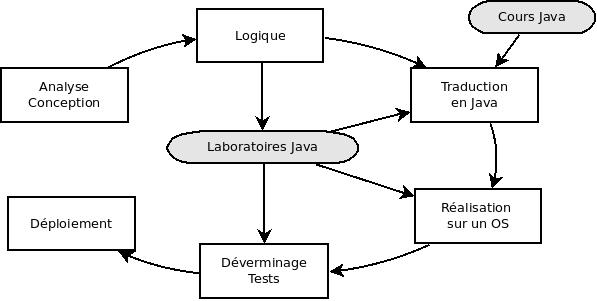
\includegraphics[scale=.5]{../img/etapes-SI} 
\end{center}
\end{frame}

\begin{frame}{Objectif secondaire}
Familiarisation avec le \emph{syst�me d'exploitation} 
(\textit{Operating System})
\emph{Linux}
\begin{itemize}
\item Pas vu au cours
\item Mais utilis� lors des \emph{laboratoires}
\item �tre capable de l'utiliser dans les t�ches courantes de programmation
\end{itemize}
\end{frame}

\subsection{Moyens}

\begin{frame}{Les supports d'apprentissage}
\emph{Pas de syllabus} pour ce cours
\begin{itemize}
  \item De nombreux livres dans le commerce
  \item Les transparents sont disponibles
\end{itemize}
\bigskip
Importance d'un \emph{livre d'accompagnement}
\begin{itemize}
\item Attention : Certains se concentrent sur 
  \begin{itemize}
  \item un aspect bien particulier du langage 
  \item une API sp�cifique
  \end{itemize}
\end{itemize}
\end{frame}

\begin{frame}[fragile]{Les ressources \textit{en ligne}}
De nombreuses ressources sur \emph{po�SI} 
\begin{itemize}
\item la \emph{plateforme d'apprentissage} de l'�SI
\item \code|elearning.esi.heb.be|
\item On y trouve : notes de cours, r�f�rences, \dots
\end{itemize}
\bigskip
Voir aussi le \emph{forum}
\begin{itemize}
\item \code|fora.namok.be|
\item Consult� par des professeurs et des �l�ves
\item Permet
  \begin{itemize}
  \item de se tenir au courant des derni�res nouvelles
  \item d'aider ou de se faire aider en cas de probl�me
  \end{itemize}
\end{itemize}
\end{frame}

\begin{frame}{Le probl�me de l'anglais}
Une connaissance de l'\emph{anglais technique} est \\primordiale
\begin{itemize}
\item Messages d'erreurs 
\item Documentation 
\end{itemize}
\bigskip
Nous essayerons d'introduire chaque nouveau terme dans les deux langues.
\end{frame}

\subsection{�valuations}

\begin{frame}{L'�valuation}
Deux \emph{cotes diff�rentes}
\begin{itemize}
\item Une pour la partie \emph{cours}
\item Une autre pour la partie \emph{laboratoire}
\end{itemize}
\bigskip
\warning{On peut donc r�ussir une partie et pas l'autre.}
\end{frame}

\begin{frame}{L'�valuation du cours}
Uniquement un \emph{oral} en fin d'ann�e
\\\bigskip
Qu'est-ce qu'on attend de vous ?
\begin{itemize}
\item \emph{Comprendre} les concepts abord�s au cours 
 \\ (\emph{pas} de \emph{<<par coeur>>})
\item Pouvoir les expliquer clairement
\item Pouvoir les illustrer au travers d'exemples courts
\item De la \emph{rigueur} : pas d'<<� peu pr�s>>
\item Du \emph{d�tail} : ne pas s'arr�ter � l'<<usage courant>>
\end{itemize}
\end{frame}

\begin{frame}{L'�valuation des laboratoires}
\emph{�valuations continues} pendant les laboratoires
\begin{itemize}
\item Courtes interrogations en \emph{d�but de s�ance}
\item Interrogations de \emph{synth�se}
\item Un \emph{projet}
\end{itemize}
\bigskip
Un examen en fin d'ann�e permet de \emph{remettre en jeu} la cote d'ann�e.
\\\bigskip
Qu'est-ce qu'on attend de vous ?
\begin{itemize}
\item De la \emph{rigueur}
\item De l'\emph{autonomie}
\end{itemize}
\end{frame}

% === Cours de Java
% === Chapitre : Introduction
\section{Programme et langage}
\leconwithtocquote{\og\ I really hate this darn machine;
\\I wish that they would sell it.
\\It won't do what I want it to,
\\but only what I tell it. \fg
\\Auteur inconnu}

\subsection{Concepts}

\begin{frame}{D�finitions}
Pouvez-vous d�finir les concepts suivants :
\begin{itemize}
\item Un \emph{programme} ?
\item \emph{Programmer} ?
\item Un \emph{langage de programmation} ? 
\item Diff�rence entre \emph{langue} et \textit{langage} ?
\end{itemize}
\end{frame}

\begin{frame}{D�finitions}
\begin{description}
\item[Langage]{ 
"Ensemble de caract�res, de symboles et de r�gles permettant de les assembler, utilis� pour donner des \emph{instructions} � l'ordinateur" (Larousse) 
}
\bigskip
\item[Programme]{ 
"S�quence d'\emph{instructions} et de donn�es enregistr�es sur un support et susceptible d'�tre trait�e par un ordinateur" (Larousse) 
}
\end{description}
\end{frame}

\begin{frame}{Cassons un mythe}
\begin{center}
\emph{\og\ Elle est b�te cette machine, \\elle s'est encore plant�e ! \fg}
\end{center}
\par\medskip
Que penser de l'\textit{intelligence} d'un ordinateur ? 
\pause
\par\medskip
R�ponse de E. Dijkstra : 
\begin{center}
\emph{\og\ Se demander si un ordinateur peut penser, 
c'est aussi int�ressant que se demander si un sous-marin peut nager. \fg}
\end{center}
\end{frame}

\begin{frame}{Un programme}
La seule chose dont est capable un ordinateur est de r�aliser ext�mement rapidement des instructions �l�mentaires
\par\bigskip
Toute t�che qu'on veut lui confier doit donc �tre pr�alablement d�crite comme une suite s�quentielle d'instructions (un programme)
\end{frame}

\begin{frame}{Un programme}
\emph{Ex:} Taille de quelques programmes
  \begin{itemize}
  \item Firefox : 2 millions de lignes de code
  \item Windows XP : 40 millions de lignes de code
  \item Mac OS X : 86 millions de lignes de code
  \item Distribution Debian 4 : 283 millions de lignes de code
  \end{itemize}
{\small(source: \code|http://en.wikipedia.org/wiki/Source_lines_of_code|)}
\end{frame}

\subsection{Historique}

\begin{frame}{Historique des langages}
\begin{description}
\item[Langage machine] : ensemble de 0 et de 1 
\item[Assemblage] : abstraction des instructions 
\item[Haut niveau (60')] : abstraction des expressions 
\\(ex: \sigle{COBOL}, \sigle{FORTRAN}) 
\item[Structur� (70')] : abstraction des structures de contr�le
\\(ex: \sigle{Pascal}, \sigle{C}) 
\item[Orient� objet (90')] : abstraction des donn�es
\\(ex: \sigle{Eiffel}, \sigle{Java}, \sigle{C++}) 
\end{description}
\end{frame}

\begin{frame}{Historique des langages}
On a aussi les langages : 
  \begin{itemize}
    \item logiques : \sigle{Prolog}, \dots
    \item fonctionnels : \sigle{Lisp}, \sigle{Scheme}, \dots
    \item orient�s aspects : \sigle{AspectJ}, \dots
  \end{itemize} 
\bigskip
\emph{Une classe de langages est adapt�e � une classe de probl�mes \dots\ et ces probl�mes �voluent dans le temps \dots}
\end{frame}

\begin{frame}{Les langages orient�s objets}
Rest�s longtemps dans les laboratoires 
  \begin{itemize}
  \item Probl�mes d'efficacit�
  \item Indigence des IDE
  \item Rupture avec les m�thodes d'analyses
  \end{itemize} 
\bigskip
Ont explos� il y a une dizaine d'ann�es \\(crise du logiciel)
  \begin{itemize}
  \item Lien avec UML
  \item �criture dans les termes du probl�me
  \item R�utilisabilit�
  \end{itemize} 
\end{frame}

\subsection{Traduction}

\begin{frame}{Le probl�me de la traduction}
Un ordinateur ne comprend que le langage machine
\begin{itemize}
\item Et un autre langage (comme \sigle{Java}) ?
\item N�cessit� d'une \emph{traduction}
\end{itemize}
\begin{center}
\begin{tabular}{c|c}
\emph{Compilation} & \emph{Interpr�tation} \\ \hline
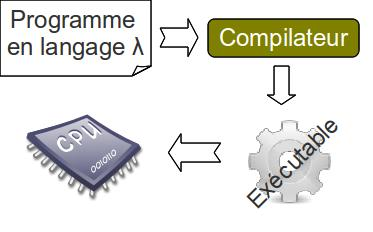
\includegraphics[scale=.35]{../img/java-jvm-compil} &
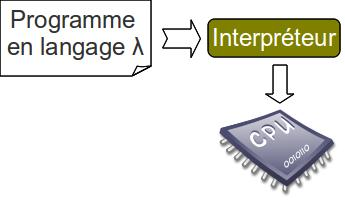
\includegraphics[scale=.35]{../img/java-jvm-interp} \\
\textit{\small traduit d'une traite} & \textit{\small traduit morceau par morceau} \\
\textit{\small avant l'ex�cution} & \textit{\small au moment de l'ex�cution} \\
\end{tabular} 
\end{center}
\end{frame}

\begin{frame}{Compilation vs interpr�tation}
Quelle est la meilleure technique au niveau de :
  \begin{itemize}
  \item La facilit� de distribution ?
  \item La rapidit� ?
  \item La facilit� de d�veloppement ?
  \end{itemize} 
\end{frame}


% === Cours de Java
% === Chapitre : Introduction
\section{Et \sigle{Java} dans tout �a ?}
\leconwithtoc

\subsection{Historique}

\begin{frame}[fragile]{Historique de \sigle{Java}}
\begin{itemize}
\item [\emph{92}] \sigle{SUN} cr�e \sigle{oak} (syst�mes embarqu�s).
\\Auteur: James Gosling
\item [\emph{94}] Adapt� � Internet gr�ce aux \emph{applets}. 
\\Devient \sigle{Java}
\item [\emph{96}] Premi�re version stable et gratuite de \sigle{JDK} 
\item [\emph{98}] Sortie de \sigle{Java 2}
\item [\emph{05}] Version \verb|1.5| de \sigle{Java 2}
\item [\emph{09}] \sigle{Oracle} rach�te \sigle{Sun} (et donc \sigle{Java})
\item [\emph{11}] Version \verb|1.7| (Java 7, en GPL) 
\includegraphics[scale=.5]{../img/java7.jpeg}
\end{itemize}
\end{frame}

\subsection{Les �ditions de \sigle{Java}}

\begin{frame}{Les �ditions de \sigle{Java}}
\emph{Java} est disponible en 3 \emph{�ditions}
  \begin{itemize}
  \item M�me langage
  \item Mais taille de la biblioth�que diff�rente
  \item Adapt� � des situations diff�rentes
  \end{itemize}
\bigskip
\emph{Java SE} (�dition standard)
  \begin{itemize}
  \item Applications monopostes classiques
  \item Les applications Android sont en Java
  \end{itemize}
\end{frame}

\begin{frame}{Les �ditions de \sigle{Java}}
\emph{Java ME} (�dition mobile - plus l�ger) 
  \begin{itemize}
  \item Applications \emph{embarqu�es} : t�l�phones, appareils �lectroniques, \dots
  \item Omnipr�sent
  \end{itemize}
\medskip
\emph{Java EE} (�dition entreprise - plus complet)
  \begin{itemize}
  \item Applications distribu�es : client-serveur, web
  \item Tr�s pr�sent : riche, robuste et portable
  \item Concurrents : \sigle{.NET} (\sigle{Microsoft}), \sigle{PHP}
  \end{itemize}
\end{frame}

\subsection{Pourquoi \sigle{Java} ?}
 
\begin{frame}{Pourquoi \sigle{Java} ?}
R�elles \emph{qualit�s p�dagogiques}  
  \begin{itemize}
  \item Syntaxe claire et pr�cise
  \item Typage fort
  \item D�tection pr�coce des erreurs
  \item Concepts modernes de programmation 
  \item �conomie d'�chelle
  \end{itemize}
\bigskip
A trouv� sa place dans le milieu professionnel
\end{frame}

\begin{frame}{\sigle{Java} et les autres langages}
Vous verrez d'autres langages
  \begin{itemize}
  \item Assembleur en premi�re 
  \item \sigle{C} et \sigle{C++} en deuxi�me 
  \item \sigle{Cobol} en 1�re, 2�me et 3�me (Gestion)
  \end{itemize}
\bigskip
Vous approfondirez Java
  \begin{itemize}
  \item Les ateliers logiciels, applications distribu�es
  \end{itemize}
\end{frame}

% === Cours de Java
% === Chapitre : Introduction
\section{D�velopper en \sigle{Java}}
\leconwithtoc

\subsection{La machine virtuelle}

\begin{frame}{Le probl�me de la portabilit�}
Il est difficile de d�velopper un programme \textit{multi-OS}
  \begin{itemize}
  \item Parties de code diff�rentes d'un OS � l'autre
  \item $\Longrightarrow$ ne tourne que sur un OS
  \end{itemize} 
\medskip
Intenable pour \sigle{Java} (\emph{applets})
  \begin{itemize}
  \item N�cessit� de developper un code \emph{portable}
  \end{itemize}
\medskip
R�ponse de \sigle{SUN} : la machine \emph{virtuelle} (JVM)
  \begin{itemize}
  \item Programmes \sigle{Java} d�velopp�s pour la JVM
  \item Comment les faire tourner sur une machine r�elle ?
  \end{itemize}
\end{frame}

\begin{frame}{La machine virtuelle}
Via un programme qui \emph{�mule} la \emph{machine virtuelle \sigle{Java}} (\sigle{JVM})  
\medskip
\begin{center}
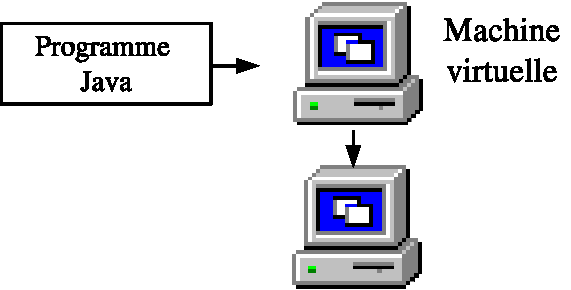
\includegraphics[scale=.8]{../img/java-jvm-jvm1} 
\end{center} 
\end{frame}

\begin{frame}{La machine virtuelle}
\sigle{Java} serait lent � interpr�ter (langage de haut niveau)
\begin{itemize}
\item Introduction d'un niveau interm�diaire : le \emph{\sigle{Bytecode}}
  \begin{itemize}
  \item Proche d'un langage d'assemblage
  \item Plus rapide � interpr�ter
  \item C'est en fait le langage de la \sigle{JVM} 
  \end{itemize}
\item \sigle{Java} est d'abord compil� en \sigle{Bytecode}
\end{itemize}
\bigskip
$\Longrightarrow$ \emph{Approche mixte} compilation/interpr�tation
\end{frame}

\begin{frame}{La machine virtuelle}
\begin{center}
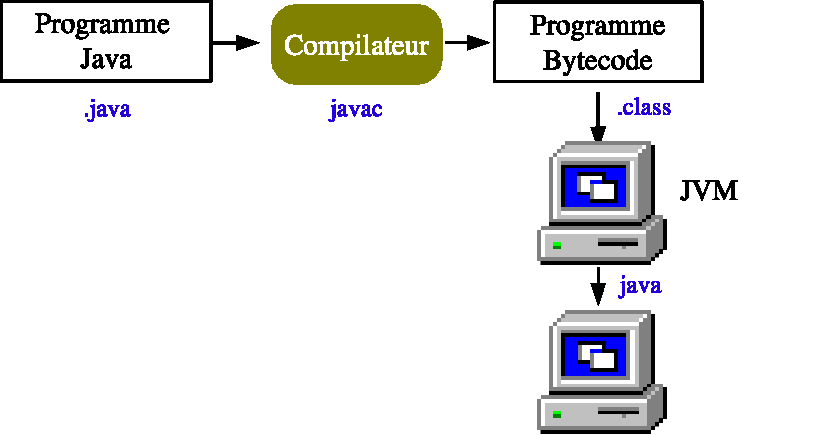
\includegraphics[scale=0.8]{../img/java-jvm-jvm2} 
\end{center}
\end{frame}

\begin{frame}[fragile]{Exemple: premier programme}
Prenons un exemple \textit{(fichier \code{Hello.java})}
\begin{Java}
// Mon premier programme
public class Hello {
  public static void main(String[] args) {
    System.out.println("Bonjour !");
  }
}
\end{Java}
\raisebox{2ex}{Compilons-le}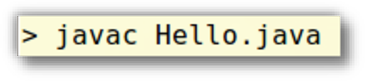
\includegraphics[scale=.8]{../img/javac} \raisebox{2ex}{\scriptsize(extrait d'une console)}\\
On obtient la version compil�e (\code|Hello.class|)\\
\raisebox{3ex}{Ex�cutons-la sur la machine virtuelle}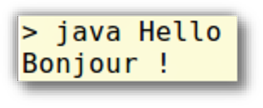
\includegraphics[scale=.8]{../img/java}
\end{frame}

\subsection{Les outils de d�veloppement}

\begin{frame}{Les outils de d�veloppement}
\emph{\sigle{JRE}} : \textit{Java Runtime Environment}
\begin{itemize}
\item Ce qui est n�cessaire � l'ex�cution
\item Accompagne les navigateurs \sigle{Web} par ex.
\end{itemize}
\bigskip
\emph{\sigle{JDK SE}} : \textit{Java Development Kit} (standard edition)
\begin{itemize}
\item Permet de developper en Java
  \begin{itemize}
  \item \emph{\sigle{javac}} : compilateur \sigle{Java} vers \sigle{bytecode}
  \item \emph{\sigle{java}} : la machine virtuelle \sigle{Java} 
  \item \emph{\sigle{javadoc}} : production automatique de documentation
  \item \dots
  \end{itemize}  
\item Gratuit, fourni par \sout{\sigle{SUN}} \sigle{Oracle}
\end{itemize}
\end{frame}

\begin{frame}{Les outils de d�veloppement}
Les \textit{\emph{E}nvironnement de \emph{D}�veloppement \emph{I}nt�gr�} : 
\emph{\sigle{Netbeans}}, \emph{\sigle{Eclipse}}, \dots
\begin{itemize}
\item Gratuits
\item Avantages
  \begin{itemize}
  \item �diteur, compilateur, d�buggeur et aide int�gr�s dans un m�me outil
  \item G�n�ration automatis�e de code 
  \end{itemize}
\item Inconv�nient : on maitrise moins tout le processus (quand �a ne marche pas, on ne comprend pas pourquoi !)
\end{itemize}
\end{frame}

\begin{frame}{Les outils de d�veloppement}
Autre possibilit� : les techniques brutes
\begin{itemize}
\item Un \emph{�diteur avec coloration syntaxique}
\item Gestion manuelle des noms et emplacements des fichiers
\item Compilation et ex�cution en ligne de commande
\end{itemize}
\bigskip
\begin{center}
\textit{Approche choisie � l'�cole pour vous faire \\comprendre ce qu'il y a derri�re}
\end{center}
\end{frame}


% === Cours de Java
% === Chapitre : Survol 

\section{Algorithmes s�quentiels (survol)}

\leconwithabstracttoc{Nous voyons comment traduire les algorithmes s�quentiels que vous �crivez au cours de Logique}

\subsection{Structure g�n�rale d'un programme}

\begin{frame}[fragile]{Structure g�n�rale du programme}
\begin{Java}
  public class NomClasse {
    // Mettre ici les modules (on dit m�thode en Java)
  }
\end{Java}
\begin{itemize}
\item Le nom commence par une majuscule
\item Doit se trouver dans le fichier \code|NomClasse.java|
\end{itemize}
\bigskip
\emph{Attention !} En \sigle{Java} : minuscule $\neq$ majuscule
\par\medskip
\emph{Exemple} : on ne peut pas �crire
\begin{Java}
  Public CLASS NomClasse {
    
  }
\end{Java}
\end{frame}

\begin{frame}[fragile]{La m�thode principale}
\begin{Java}
  public class NomClasse {
    public static void main(String[] args) {
      // Code de la m�thode ici     
    }
  }
\end{Java}
\begin{itemize}
\item \java|main| est le nom de la m�thode principale
\item C'est par l� que commence le programme
\item \`A �crire tel quel, on verra pourquoi
\end{itemize}
\end{frame}

\subsection{Variables, calculs et assignation}

\begin{frame}[fragile]{Les variables}
Les types disponibles
\begin{center}
\begin{tabular}{r|l}
En Logique & En  Java \\ \hline
Entier & \java|int| \\ 
R�el & \java|double| \\ 
Chaine & \java|String| \\ 
Caract�re & \java|char| \\ 
Bool�en & \java|boolean| \\  
\end{tabular} 
\end{center}
Exemple de d�claration
\begin{Java}
   int nb1;
\end{Java}
\end{frame}

\begin{frame}[fragile]{L'assignation et les calculs}
L'assignation se fait via le symbole \java|=|
\begin{Java}
   nb1 = 1;
\end{Java}
\bigskip
Les calculs : on dispose de tous les op�rateurs \textit{classiques}
    \\\medskip
    \begin{tabular}{r|l}
    \java|+| & plus \\ 
    \java|-| & moins \\ 
    \java|*| & fois \\ 
    \java|/| & au moins 1 r�el $\Longrightarrow$ division \emph{r�elle} \\
             & 2 entiers $\Longrightarrow$ division \emph{enti�re} (\sigle{DIV} en \sigle{Logique})\\ 
             
    \java|%| & reste (\sigle{MOD} en \sigle{Logique})\\ 
    \end{tabular} 
\end{frame}

\begin{frame}[fragile]{Exemple}
\begin{Java}
  public class Moyenne {
    public static void main(String[] args) {

      int nombre1;
      int nombre2;
      int moyenne;

      nombre1 = 34345;
      nombre2 = -3213213;
      moyenne = (nombre1 + nombre2) / 2;    
      System.out.println(moyenne); 
    }
  }
\end{Java}
\end{frame}

\begin{frame}[fragile]{Exemple}
\begin{Java}
  public class Moyenne {
    public static void main(String[] args) {

      int nombre1 = 34345;
      int nombre2 = -321321;
      double moyenne;

      // division r�elle car un des 2 op�randes est r�el
      moyenne = (nombre1 + nombre2) / 2.0;    
      System.out.println("La moyenne est " + moyenne); 
    }
  }
\end{Java}
\end{frame}

\subsection{Lire au clavier}

\begin{frame}[fragile]{Lire au clavier}
Moins direct que l'affichage � l'�cran
  \begin{itemize}
  \item Applications modernes (graphiques)
  \item Lectures dans des champs de saisie
  \item Parfois utile : test ou apprentissage
  \end{itemize}
\emph{Exemple}
  \begin{Java}
  import java.util.Scanner;
  // ...
  Scanner clavier = new Scanner(System.in);
  // ...
  nombre1 = clavier.nextInt();
  \end{Java}
\end{frame}

\begin{frame}[fragile]{Lire au clavier - Exemple}
\begin{Java}
import java.util.Scanner;

public class Test {
  public static void main(String[] args) {
      Scanner clavier = new Scanner(System.in);
      double nombre1;
      double nombre2;
      double moyenne;

      nombre1 = clavier.nextDouble();
      nombre2 = clavier.nextDouble();
      moyenne = (nombre1 + nombre2) / 2.0;
      System.out.println(moyenne);    
  }
}
\end{Java}
\end{frame}

\begin{frame}{Lire au clavier}
\begin{center}
\begin{tabular}{r|l}
Pour lire\dots & on �crit\dots \\ \hline
un entier & \java|nextInt()| \\ 
un r�el & \java|nextDouble()| \\ 
un bool�en & \java|nextBoolean()| \\ 
un mot & \java|next()|\\  
une ligne & \java|nextLine()|\\  
un caract�re & \java|next().charAt(0)| \\ 
\end{tabular} 
\end{center}
\end{frame}

\subsection{Constantes}

\begin{frame}[fragile]{Constante locale}
Clause \java|final| {} $\Rightarrow$ constante
\par\medskip
Valeur donn�e
  \begin{itemize}
  \item Soit � la d�claration 
  \item Soit par assignation ult�rieure
  \end{itemize} 
\begin{Java}
  final int X = 1;
  final int Y;
  Y = 2*X;
  X = 2; // Erreur : poss�de d�j� une valeur
  Y = 3; // Idem
\end{Java}
Pourquoi une constante au lieu d'un litt�ral ?
\end{frame}

\subsection{Conventions}

\begin{frame}{Conventions de noms}
Pour une variable :
  \begin{itemize}
  \item Tout mettre en \emph{minuscules}
  \item Sauf les d�buts de \textit{noms compos�s} en majuscule
  \end{itemize} 
\medskip
Pour une constante :
  \begin{itemize}
  \item Tout mettre en \emph{majuscules}
  \item Utiliser \java|_|  pour s�parer les mots
  \end{itemize}
\medskip
Dans tous les cas : \emph{�tre explicite}
\\(sauf abr�viations courantes)
\end{frame}

\begin{frame}[fragile]{Conventions de noms}
\emph{Exemples}
\begin{Java}
  String nom;
  int ann�eEtude;
  int nbEtudiants;
  boolean partieFinie;
  final double PI;
  final int TAUX_TVA;   
\end{Java}
\end{frame}

\subsection{Commentaires}

\begin{frame}[fragile]{Le commentaire}
  \begin{Java}
  // Commentaire sur une ligne
  /* Commentaire sur
     plusieurs lignes */
  \end{Java}
\begin{itemize}
\item Destin� aux humains
\item Sans effet sur le programme
\item N�anmoins crucial
\end{itemize}
\end{frame}



\section{L'erreur est humaine}

\leconwithabstract{Identifier, comprendre et corriger\\les erreurs d'un programme}

\begin{frame}{La r�alit� de la programmation}
Nous avons vu le processus \emph{id�al}
  \begin{itemize} 
  \item On �dite / compile / ex�cute \dots et tout \textit{\og va bien\fg}
  \end{itemize}
\medskip
Cas \emph{extr�mement rare}
  \begin{itemize} 
  \item Le programmeur est humain $\rightarrow$ faillible
  \item Vous avez s�rement d�j� tous �t� confront�s � un logiciel qui \textit{\og se plante\fg}
  \end{itemize}
\medskip
Quels types d'erreurs rencontre-t-on ?
\pause
  \begin{itemize} 
  \item Erreurs de \emph{compilation}
  \item Erreurs d'\emph{ex�cution}
    \begin{itemize} 
    \item Le programme s'arr�te
    \item Le programme a un mauvais comportement
    \end{itemize}
  \end{itemize}
\end{frame}

\begin{frame}[fragile]{Les erreurs de compilation}
Le compilateur ne comprend pas ce qu'on a �crit
\begin{itemize}
\item \emph{Impossible} pour lui de le \emph{traduire} en \textit{bytecode}
\item Messages d'erreurs pour nous aider � corriger 
\end{itemize}
\emph{Exemples} : versions modifi�es de \textit{\og Hello World\fg}
\begin{Java}
public Class Hello {
  public static void main(String[] args) {
    System.out.println("Bonjour !");
  }
}
\end{Java}
%\vspace{-1ex}
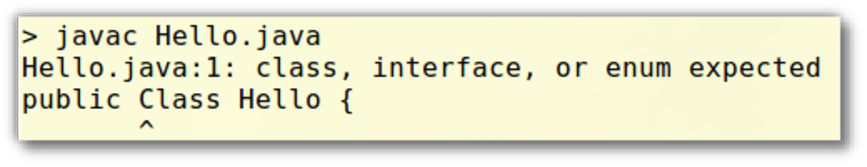
\includegraphics[scale=.7]{../img/erreur2}
%\begin{Code}
%> javac Hello.java 
%Hello.java:1: class, interface, or enum expected
%public Class Hello
%       ^
%\end{Code}
\end{frame}

\begin{frame}[fragile]{Les erreurs de compilation}
\begin{Java}
public class Hello {
  public static void main(string[] args) {
    System.out.println("Bonjour !");
  }
}
\end{Java}
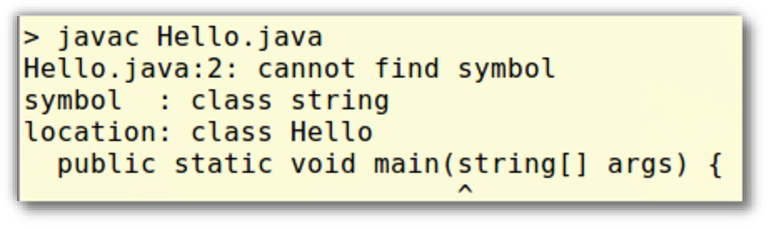
\includegraphics[scale=.7]{../img/erreur3}
%\begin{Code}
%> javac Hello.java 
%Hello.java:2: cannot find symbol
%symbol  : class string
%location: class Hello
%  public static void main(string[] args)
%                           ^
%\end{Code}
\end{frame}

\begin{frame}{Les bonnes pratiques}
Une grosse partie de la programmation consiste � \emph{d�tecter / corriger} les probl�mes
\begin{itemize}
\item Plus t�t on d�tecte une erreur, plus vite elle est corrig�e (le rapport peut �tre de 1 � 10)
\end{itemize}
\medskip
Aptitude � travailler au laboratoire
\begin{itemize}
\item C'est un \emph{savoir-faire} plus qu'un savoir
\item Suivre quelques \emph{pratiques} qui ont fait leur preuve
\end{itemize}
\end{frame}

\begin{frame}{Les bonnes pratiques}
Application aux erreurs de compilation
\begin{itemize}
\item \emph{Compiler souvent} \\(pas uniquement \og � la fin \fg)
  \begin{itemize}
  \item Moins d'erreurs � corriger � la fois
  \item Messages du compilateur plus clairs
  \item Ne b�tir que sur du solide
  \end{itemize}
\item \emph{Lire / comprendre} les messages
  \begin{itemize}
  \item Id�alement, on sait d�j� quel est le probl�me avant de retourner dans l'�dition
  \item Astuce : si beaucoup d'erreurs, commencer par les premi�res
  \end{itemize}
\item \emph{Retenir / reconnaitre} les erreurs fr�quentes
\end{itemize}
\end{frame}

\begin{frame}{Les erreurs d'ex�cution}
La JVM ne \emph{sait pas ex�cuter} une instruction
\begin{itemize}
\item S'\emph{arr�te} avec un message expliquant
  \begin{itemize}
  \item L'instruction qui pose probl�me
  \item La \emph{nature du probl�me}
  \end{itemize}
\item Comme pour la compilation : \emph{lire} / \emph{comprendre} / \emph{retenir} / \emph{reconnaitre} les erreurs
\item Afficher des \og traces\fg\ ou utiliser un \og d�buggeur\fg\ peut aider � trouver le probl�me
\end{itemize}
\end{frame}

\begin{frame}[fragile]{Les erreurs d'ex�cution}
\emph{Exemple} : Une petite division
\begin{Java}
public class Test {
  public static void main(String[] args) {
    int num�rateur = 1;
    int d�nominateur = 0;
    System.out.println( num�rateur / d�nominateur );
  }
}
\end{Java}
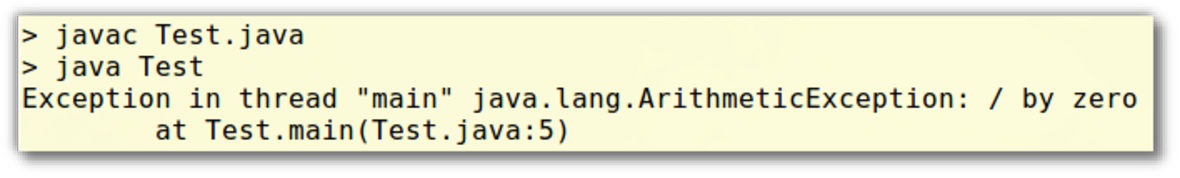
\includegraphics[scale=.6]{../img/erreur4}
%\begin{Code}
%> javac Test.java
%> java Test
%Exception in thread "main" java.lang.ArithmeticException: / by zero
%	at Test.main(Test.java:7)
%\end{Code}
\end{frame}

\begin{frame}{Les erreurs de calcul}
La r�ponse / le comportement n'est pas le bon
\begin{itemize}
\item Erreur dans notre \emph{logique} ou notre \emph{traduction}
\item Erreurs les plus \emph{pernicieuses}
  \begin{itemize}
  \item R�flexe � croire que la r�ponse est bonne
  \end{itemize}
\item \emph{Tester} son programme 
  \begin{itemize}
  \item V�rifier les r�ponses
  \item Penser aux cas \emph{limites}
  \item Nous verrons des techniques adapt�es \\(\sigle{JUnit} pour les tests unitaires)
  \end{itemize}
\end{itemize}
\end{frame}


% === Cours de Java
% === Chapitre : Survol 

\section{Alternatives (survol)}

\leconwithabstract{Nous voyons comment traduire les algorithmes contenant des alternatives que vous �crivez en logique}

\begin{frame}[fragile]{Instructions de choix}
Le \emph{Si}
\begin{Java}
  if ( condition ) {
    instructions
  }
\end{Java}
\bigskip
Le \emph{Si-sinon}
\begin{Java}
  if ( condition ) {
    instructions
  } else {
    instructions
  }
\end{Java} 
\end{frame}

\begin{frame}[fragile]{Exemple} 
\begin{Java}
import java.util.Scanner;
public class Test {
  public static void main(String[] args) {
      Scanner clavier = new Scanner(System.in);
      int nombre1;

      nombre1 = clavier.nextInt();
      if (nombre1 < 0) {
         System.out.println(nombre1 + " est n�gatif"); 
      }   
  }
}
\end{Java}
\end{frame}

\begin{frame}[fragile]{Exemple} 
\begin{Java}
import java.util.Scanner;
public class Test {
  public static void main(String[] args) {
      Scanner clavier = new Scanner(System.in);
      int nombre1;

      nombre1 = clavier.nextInt();
      System.out.println(nombre1 + " est un nombre ");
      if (nombre1 < 0) {
         System.out.println("n�gatif"); 
      } else {
         System.out.println("positif");   
      }
  }
}
\end{Java}
\end{frame}

\begin{frame}[fragile]{Exercice} 
Comment traduire cet algorithme ?
\begin{Code}
MODULE Test
    nombre1: Entier
    LIRE nombre1
    SI nombre1 > 0 ALORS
        ECRIRE nombre1, "est positif"
    SINON
        SI nombre1 = 0 ALORS
            ECRIRE nombre1, "est nul"
        SINON
            ECRIRE nombre1, "est n�gatif"
        FIN SI
    FIN SI
FIN MODULE
\end{Code}
\end{frame}

\begin{frame}[fragile]{Expressions bool�ennes} 
Pour les tests, on peut utiliser :
\begin{itemize}
\item Des comparateurs : \java|<|, \java|>|, \java|<=|, \java|>=|, \java|==|, \java|!=|
\item Des op�rateurs bool�ens : \java|&&| (et), \java{||} (ou), \java|!| (non)
\end{itemize} 
\bigskip
\emph{Attention !} Bien distinguer \java|=| et \java|==|
\end{frame}

\begin{frame}[fragile]{Exemple} 
\begin{Java}
import java.util.Scanner;
public class Exemple {
  public static void main(String[] args) {
      Scanner clavier = new Scanner(System.in);
      int nombre1;

      nombre1 = clavier.nextInt();
      if ((nombre1 % 2) == 0) {
         System.out.println("Le nombre est pair");
      } else {
         System.out.println("Le nombre est impair"); 
      }
  }
}
\end{Java}
\end{frame}

\begin{frame}[fragile]{Exemple} 
\begin{Java}
import java.util.Scanner;
public class Exemple {
  public static void main(String[] args) {
      Scanner clavier = new Scanner(System.in);
      int �ge;

      �ge = clavier.nextInt();
      if ( �ge<21 || �ge>=60 ) {
         System.out.println("Tarif r�duit !");
      }
  }
}
\end{Java}
\end{frame}

\begin{frame}[fragile]{Le \og selon-que\fg} 
Premi�re forme
\begin{Java}
  switch(num�roJour) {
    case 1 : intitul�Jour="Lundi"; break;
    case 2 : intitul�Jour="Mardi"; break;
    case 3 : intitul�Jour="Mercredi"; break;
    case 4 : intitul�Jour="Jeudi"; break;
    case 5 : intitul�Jour="Vendredi"; break;
    case 6 : intitul�Jour="Samedi"; break;
    case 7 : intitul�Jour="Dimanche"; break;
    default : intitul�Jour="Inconnu"; break;
  }
\end{Java}
\begin{itemize}
\item Notez le \java{break}
\item Possible avec : entiers, caract�res et chaines
\end{itemize}
\end{frame}

\begin{frame}[fragile]{Le \og selon-que\fg} 
Deuxi�me forme : la logique suivante
\begin{Code}
  Selon que 
    nb > 0 : Ecrire "positif"
    nb = 0 : Ecrire "nul"
    autrement : Ecrire "n�gatif"
  Fin selon que
\end{Code}
s'�crit en Java
\begin{Java}
  if (nb>0) {
      System.out.println("positif");
  } else if (nb==0) {
      System.out.println("nul");
  } else {
      System.out.println("n�gatif");
  }  
\end{Java}
\end{frame}


% === Cours de Java
% === Chapitre : La grammaire
\section{La notion de grammaire}

\leconwithtoc

\subsection{La notion de grammaire}

\begin{frame}{Le besoin d'une r�f�rence}
Un langage de programmation doit pouvoir
  \begin{itemize}
  \item \emph{�tre d�crit} aupr�s des programmeurs
  \item faire l'objet d'une \emph{compilation rigoureuse}
  \end{itemize} 
\medskip\pause
Il faut un \emph{document de r�f�rence}
  \begin{itemize}
  \item Pour Java : \emph{The Java Language Specification}
    \begin{itemize}
    \item Contient beaucoup de texte (en \emph{Anglais})
    \item Ce qui est parfois \emph{incomplet} / \emph{ambigu}
    \end{itemize} 
  \end{itemize}
\medskip\pause
N�cessit� d'utiliser un \emph{formalisme} pr�cis
  \begin{itemize}
  \item En Logique : LDA
  \item En Analyse : UML
  \item En Langage : une \emph{grammaire} 
  \end{itemize} 
\end{frame}

\begin{frame}{La notion de grammaire}
Une grammaire est une description \emph{finie} de l'\emph{infinit�} des programmes corrects
\begin{center}
programme $\equiv$ phrase $\supset$ mots $\supset$ caract�res
\end{center} 
\begin{itemize}
\item Chaque \emph{mot} (on dit \emph{token} en informatique) doit �tre l�gal
  \begin{itemize}
  \item d�termin� par une \emph{grammaire lexicale}
  \end{itemize} 
\item \emph{S�quence de mots} doit �tre l�gale
  \begin{itemize}
  \item d�termin� par une \emph{grammaire syntaxique}
  \end{itemize}
\item La \emph{s�mantique} ne peut pas �tre d�crite aussi rigoureusement 
\end{itemize}
\end{frame}

\begin{frame}{La notion de grammaire}
Parall�le avec une \emph{langue naturelle}
\\(dictionnaire, grammaire)
\\\bigskip\emph{Exemples}
  \begin{itemize}
  \item \textit{<<El tahc tse rion>>} 
  \item \textit{<<Le est chat noir>>}
  \item \textit{<<Le chat est noir>>}
  \item \textit{<<Le parapluie mange l'ascenceur>>}
  \end{itemize} 
\end{frame}

\subsection{Comment fonctionne une grammaire ?}

\begin{frame}{Comment fonctionne une grammaire ?}
Une grammaire est compos�e de
\begin{itemize}
\item l'ensemble des tokens pouvant apparaitre tels quels (\textit{symboles \emph{terminaux}})
\item l'ensemble des \emph{r�gles de production}
  \begin{itemize}
  \item nom de la r�gle (\textit{symbole \emph{non terminal}})
  \item s�quences de symboles produits par la r�gle 
  \end{itemize}
\item une r�gle de production de \emph{d�part} 
\end{itemize}
\begin{center}
Est \emph{valide} ce qui peut �tre \emph{produit} par la grammaire
\end{center}
\end{frame}

\begin{frame}{Comment fonctionne une grammaire ?}
Pour la grammaire \emph{syntaxique}
  \begin{itemize}
  \item les symboles terminaux sont les mots
  \item les r�gles construisent la phrase 
  \end{itemize}
\bigskip
Pour la grammaire \emph{lexicale}
  \begin{itemize}
  \item les symboles terminaux sont les caract�res
  \item les r�gles construisent le mot 
  \end{itemize}
\bigskip
Pourquoi ne pas utiliser un dictionnaire pour les mots ?
\end{frame}

\begin{frame}[fragile]{Exemple : le langage MU}
Inventons un nouveau langage : le \emph{langage MU}
\begin{itemize}
\item Nous devons indiquer de mani�re pr�cise quelle phrase est valide dans notre langage
\item Cela se fait en donnant sa grammaire
\pause
  \begin{itemize}
  \item Les 3 symboles terminaux: \texttt{M},\texttt{U},\texttt{I}
  \item Les 3 r�gles de production
  \begin{small}
\begin{verbatim}
  start:
       debut MU fin

  debut:                   fin:
       debut I                I fin
       I                      I 
\end{verbatim}
  \end{small}
  \item La r�gle de d�part : \texttt{start}
  \end{itemize}
\end{itemize}
\end{frame}


\begin{frame}{Exemple : le langage MU}
Quelques \emph{phrases correctes} (qu'on peut \textit{produire}) 
  \begin{itemize}
  \item \texttt{IMUI}
  \item \texttt{IIMUI}
  \item \texttt{IMUIIIIIIIIIIIIIIIIIIIIIIIII}
  \item \dots � l'infini
  \end{itemize} 
\medskip \pause
Quelques \emph{phrases incorrectes} (impossibles � \textit{produire}) 
  \begin{itemize}
  \item \texttt{MU}
  \item \texttt{MUI}
  \item \texttt{MUIMU}
  \item \dots � l'infini
  \end{itemize} \end{frame}

\begin{frame}[fragile]{Exemple}
Voici un autre exemple
\begin{itemize}
\item Le symbole terminal: \texttt{A}
\item Les 2 r�gles de production
\begin{verbatim}
  liste:
       element
       element liste
  element:
       A  
\end{verbatim}
\item La r�gle de d�part : \texttt{liste}
\end{itemize}
\bigskip
Quel est le langage produit par cette grammaire ?
\end{frame}

\subsection{Notations de la grammaire \sigle{Java}}

\begin{frame}[fragile]{Notations de la grammaire \sigle{Java}}
Une r�gle de la grammaire syntaxique java:
\begin{grammaire}
\nterm{ReturnStatement} :
     \term{return} Expression\opt;
\end{grammaire}
\begin{itemize}
\item Imaginez des exemples d'instruction \og return\fg\ valides
\end{itemize}
\bigskip
La \emph{grammaire compl�te} de \sigle{Java} 
peut �tre consult�e dans le livre
\textit{\og The Java Language Specification\fg}
\end{frame}

% === Cours de Java
% === Chapitre : La grammaire
\section{La grammaire lexicale de Java}

\leconwithtoc

\subsection{Analyse lexicale}

\begin{frame}{Analyse lexicale de Java}
 Premi�re phase d'analyse d'un programme
\begin{itemize}
\item Examine la s�quence des caract�res d'entr�e
\item Supprime \texttt{caract�res d'espacement} et \texttt{commentaires}
\item Identifie les \textit{tokens} (mots) du langage 
\end{itemize} 
\begin{center}
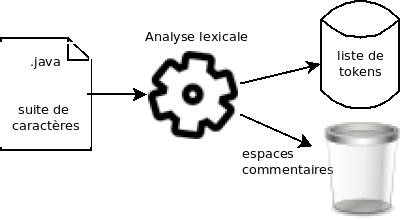
\includegraphics[scale=.5]{../img/phase1} 
\end{center} 
\end{frame}

\begin{frame}{Analyse lexicale de Java}
L'analyse lexicale se base sur une grammaire lexicale
\begin{itemize}
\item Les symboles \texttt{terminaux} sont l'ensemble des caract�res \sigle{Unicode}
\end{itemize} 
\bigskip
\sigle{Java} a fait le choix de l'\sigle{UTF-16} (\sigle{Unicode})
  \begin{itemize}
  \item \sigle{ASCII}: 7 bits
  \item \sigle{ASCII �tendu}: 8 bits
  \item \sigle{EBCDIC}: 8 bits (\sigle{IBM})
  \item \sigle{UTF-16}: 2 bytes, 16 bits 
\\(les 128 premiers caract�res $\equiv$ \sigle{ASCII}) 
  \end{itemize}
\end{frame}

\begin{frame}[fragile]{Les s�quences Unicode}
Java permet une repr�sentation \sigle{ASCII} de tout caract�re \sigle{UTF-16} (via un \textit{caract�re d'�chappement})
\begin{itemize}
\item \emph{Ex} : le caract�re \emph{p} peut aussi s'�crire \code{\u0070} 
\item Une traduction pr�alable est r�alis�e :
\end{itemize}
\begin{Java}
\u0070ublic class MaClasse
\end{Java}
devient
\begin{Java}
public class MaClasse
\end{Java}
\end{frame}

\begin{frame}[fragile]{Les caract�res d'entr�e}
\begin{grammaire}
\nterm{UnicodeInputCharacter} :
   \nterm{UnicodeEscape}
   \nterm{RawInputCharacter}

\nterm{UnicodeEscape} :
   \term{\textbackslash}\nterm{UnicodeMarker} \nterm{HexDigit} \nterm{HexDigit} \nterm{HexDigit} \nterm{HexDigit}

\nterm{UnicodeMarker} :
   \term{u}
   \nterm{UnicodeMarker} \term{u}

\nterm{RawInputCharacter} :
   any Unicode character

\nterm{HexDigit} : one of
   \term{0}  \term{1}  \term{2}  \term{3}  \term{4}  \term{5}  \term{6}  \term{7}  \term{8}  \term{9}    \term{a}  \term{b}  \term{c}  \term{d}  \term{e}  \term{f}     \term{A}  \term{B}  \term{C}  \term{D}  \term{E}  \term{F}  
\end{grammaire}
\end{frame}

\subsection{Les espaces}

\begin{frame}[fragile]{Les caract�res d'espacement}
Les <<espaces>> n'ont pas de sens en \sigle{Java}
\begin{itemize}
\item Peuvent �tre utilis�s librement entre les mots
\item Mais ne peuvent pas couper un mot
\item Exception : les chaines (\textit{String})
\end{itemize}
\begin{grammaire}[basicstyle=\scriptsize]
\nterm{WhiteSpace} :
   the ASCII SP character, also known as "space"
   the ASCII HT character, also known as "horizontal tab"
   the ASCII FF character, also known as "form feed" 
   \nterm{LineTerminator}

\nterm{LineTerminator} :
   the ASCII LF character, also known as "newline"
   the ASCII CR character, also known as "return"
   the ASCII CR character followed by the ASCII LF character
\end{grammaire} 
\end{frame}

\subsection{Les commentaires}

\begin{frame}[fragile]{Le commentaire}
  \begin{itemize}
  \item Sur 1 ligne
    \begin{Java}
// Commentaire sur 1 ligne
    \end{Java}
  \item Sur plusieurs lignes
    \begin{Java}
/* Exemple de commentaire
   sur plusieurs lignes */
    \end{Java}
    \begin{Java}
/** Pour un commentaire Javadoc */
    \end{Java}
  \item Ne peuvent pas �tre imbriqu�s
  \item N'importe o� \textbf{entre} les mots  
  \end{itemize}
\end{frame}

\subsection{Les tokens}

\begin{frame}[fragile]{Les tokens (mots du langage)}
Les caract�res qui restent vont former les \textit{tokens} (mots, symboles terminaux)
\begin{itemize}
\item 5 sortes de tokens 
\begin{grammaire}
\nterm{Token} : one of
    \nterm{Identifier}  \nterm{Literal}  \nterm{Keyword}  \nterm{Separator}  \nterm{Operator}
\end{grammaire}
\end{itemize}
\end{frame}

\begin{frame}[fragile]{Les tokens (mots du langage)}
Liste des \nterm{keyword} (\emph{mots-cl�s} ou r�serv�s)
\begin{grammaire}
\nterm{Keyword} : one of
   \term{abstract}   \term{boolean}   \term{break}   \term{byte}   \term{case}   \term{catch}   
   \term{char} \term{class}   \term{const}   \term{continue}   \term{default}   \term{do}   
   \term{double}   \term{else} \term{extends}   \term{final}   \term{finally}   \term{float}   
   \term{for}   \term{goto}   \term{if} \term{implements}   \term{import}   \term{instanceof}    
   \term{int}   \term{interface} \term{long}   \term{native}   \term{new}   \term{package}   
   \term{private}   \term{protected} \term{public}   \term{return}   \term{short}   
   \term{static}  \term{super}   \term{switch} \term{synchronized}  \term{this}   \term{throw}   
   \term{throws}   \term{transient} \term{try}   \term{void}   \term{volatile}   \term{while}
\end{grammaire}
\end{frame}

\begin{frame}[fragile]{Les tokens (mots du langage)}
Les identifiants
\begin{grammaire}
\nterm{Identifier} :
   \nterm{IdentifierChars} 
         but not a \nterm{Keyword} or \nterm{BooleanLitteral} or \nterm{NullLitteral}

\nterm{IdentifierChars} :
   \nterm{JavaLetter} 
   \nterm{IdentifierChars} \nterm{JavaLetterOrDigit}

\nterm{JavaLetter} :
   any Unicode character that is a Java letter (_ et \$ sont compris)

\nterm{JavaLetterOrDigit} :
   any Unicode character that is a Java letter-or-digit 
\end{grammaire}
(cf. la grammaire compl�te pour les d�tails)
\end{frame}

\begin{frame}[fragile]{Les tokens (mots du langage)}
Liste des s�parateurs et op�rateurs
\begin{grammaire}
\nterm{Separator} : one of
    \term{(}  \term{)}  \term{\{}  \term{\}}  \term{[}  \term{]}  \term{;}  \term{,}  \term{.}

\nterm{Operator} : one of
    \term{=}   \term{>}   \term{<}   \term{!}   \term{~}   \term{?}   \term{:}  \term{==}   \term{<=}   \term{>=}   \term{!=}   \term{&&}   \term{||}   
    \term{++}   \term{--}   \term{+}   \term{-}   \term{*}   \term{/}   \term{&}   \term{|}   \term{^}   \term{%}   \term{<<}   \term{>>}   \term{>>>}
    \term{+=}   \term{-=}   \term{*=}   \term{/=}   \term{&=}   \term{|=}   \term{^=}   \term{%=}   \term{<<=}   \term{>>=}   \term{>>>=}
\end{grammaire}
Comment l'analyseur lexical va-t-il reconnaitre \java|---| ?
\end{frame}

\begin{frame}{R�capitulatif des phases de compilation}
Une fois les tokens identifi�s, le compilateur peut passer � l'analyse syntaxique et s�mantique
\begin{center}
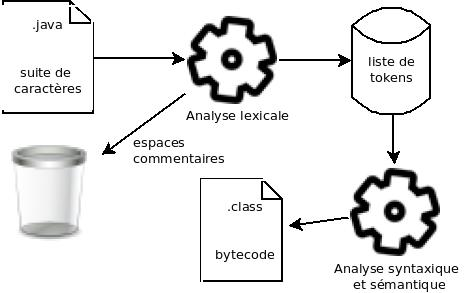
\includegraphics[scale=.5]{../img/phases} 
\end{center} 
\end{frame}


% === Cours de Java

\section{�crire du code lisible}

\leconwithabstract{Nous montrons pourquoi et comment �crire du code lisible}

\begin{frame}[fragile]{Et pourtant �a tourne !}
On a vu que le compilateur ne se pr�occupe pas de la \textit{mise en page}
\begin{itemize}
\item Tous les \textit{whitespace} sont �limin�s lors de l'analyse lexicale
(\textit{whitespace} $\equiv$ \textit{espace}, \textit{retour � la ligne}, \dots)
\end{itemize}
$\Longrightarrow$ ceci est \emph{�quivalent} au \textit{Hello World}
\begin{Java}
public
class
Hello{public static void main(String[] args){System.
out.              println( "Bonjour !"         );}}
\end{Java}
\end{frame}

\begin{frame}{Et pourtant �a tourne !}
C'est correct pour le compilateur mais � \emph{proscrire}
\begin{itemize}
\item Un code est \emph{souvent lu}
  \begin{itemize}
  \item Lorsqu'il est �crit / mis au point
  \item Correction de bug 
  \item �volution du code (les besoins changent)
  \end{itemize}
\item Et souvent par des \emph{personnes diff�rentes}
\end{itemize}
\bigskip
$\Longrightarrow$ \emph{La lisibilit� est essentielle}
\end{frame}

\begin{frame}[fragile]{Un code lisible}
\emph{R�gle 1} : \emph{Indenter} correctement son code 
  \begin{itemize}
  \item Pour un aper�u global de la structure du code
  \item Pour rep�rer rapidement la fin d'un \textit{bloc}
  \end{itemize}
\bigskip
\emph{R�gle 2} : Bien choisir le \emph{nom des variables}
\begin{itemize}
\item Ce bout de code est syntaxiquement correct
\item Mais que fait-il ?
\end{itemize}
\begin{Java}
  int u=clavier.nextInt(),n=clavier.nextInt(),
  t=clavier.nextInt();
  double p=u*n*(1+t/100.0);
  System.out.println(p);
\end{Java}
\end{frame}

\begin{frame}[fragile]{Un code lisible}
Nous lui pr�f�rons celui-ci plus lisible :
\begin{Java}                                                 
  double �Payer;
  int prixUnitaire = clavier.nextInt();
  int nombreArticles = clavier.nextInt();
  int tauxTva = clavier.nextInt();

  �Payer = prixUnitaire * nombreArticles * (1 + tauxTva/100.0);

  System.out.println(�Payer);
\end{Java}
\end{frame}

\begin{frame}{Un code lisible}
\emph{R�gle 3} : \emph{D�composer} les expressions trop longues
  \begin{itemize}
  \item Une variable interm�diaire peut accroitre la lisibilit� : le nom donne un sens � l'expression
  \item La perte de place m�moire est n�gligeable 
  \\(voire nulle car un compilateur peut optimiser) 
  \item Trop d�composer nuit parfois � la lisibilit� 
  \\(limite floue)
  \\$\Longrightarrow$ importance de l'\emph{exp�rience}
  \end{itemize}
\end{frame}

\begin{frame}[fragile]{Un code lisible}
\emph{Exemple} : reprenons l'exemple du calcul du prix � payer
\begin{Java}
  int prixUnitaireHTva = clavier.nextInt();
  int nombreArticles = clavier.nextInt();
  int tauxTva = clavier.nextInt();
  int prixUnitaireTTC = prixUnitaireHTva * (1 + tauxTva/100.0);                               
  double �Payer = prixUnitaireTTC * nombreArticles;
\end{Java}
\medskip
\emph{Exemple} : que pr�f�rer de
\begin{Java}
int hypo = sqrt( a*a + b*b );
\end{Java}
\begin{Java}
int aCarr� = a*a;
int bCarr� = b*b;
int hypo = sqrt( aCarr� + bCarr� );
\end{Java}
\end{frame}

\begin{frame}[fragile]{Un code lisible}
\emph{R�gle 4} : Utiliser des \emph{constantes}
\begin{itemize}
\item Rend le code plus lisible
\item Facilite aussi son �volution
\end{itemize}
\begin{Java}                                                 
  final double TAUX_TVA = 0.21;
  double taxe;
  double prix = clavier.nextInt();
  taxe = prix * TAUX_TVA;
  System.out.println(taxe);
\end{Java}
\end{frame}

\begin{frame}[fragile]{Un code lisible}
\emph{Anti-r�gle} : Surcharger de \emph{commentaires}
\begin{itemize}
\item Vient souvent au secours d'un code non lisible
\item Id�alement on utilisera les commentaires
  \begin{itemize}
  \item En d�but de programme, de module
  \item Pour expliquer \emph{ce qu'il fait}
  \item Mais surtout \emph{pas comment} il le fait
  \item cf. \textit{javadoc}
  \end{itemize} 
\end{itemize}
\bigskip
Il y a d'autres r�gles ? Oui !
\begin{itemize}
\item Pour \sigle{Java}, document reprenant les conventions � respecter :
{\scriptsize \code|http://www.oracle.com/technetwork/java/codeconv-138413.html|}
\end{itemize} 
\end{frame}

\begin{frame}{La refactorisation}
\emph{En r�alit�} : On n'�crit pas un code lisible du premier coup !
\\\bigskip
\emph{Refactoriser} = changer le code en vue d'am�liorer sa lisibilit� / son �volutivit� sans changer ce qu'il fait
  \begin{itemize}
  \item \emph{Exemples}
    \begin{itemize}
    \item donner un nom plus explicite � une variable
    \item mieux indenter le code
    \end{itemize}
  \item \emph{Contre-exemples}
    \begin{itemize}
    \item ajouter une fonctionnalit�
    \item r�parer un bug
    \end{itemize}
  \end{itemize}
\end{frame}

\begin{frame}{La refactorisation}
Mais refactoriser c'est toucher � du code qui fonctionne ! 
Ce n'est pas dangereux ?
\\\medskip
\emph{Oui}! $\Longrightarrow$ importance 
  \begin{itemize}
  \item des tests de \emph{non-r�gression} (cf. \sigle{JUnit})
  \item d'un syst�me de \emph{gestion des versions}
  \end{itemize}
\medskip
Pour aller plus loin : Martin Fowler, \\
<<\textit{Refactoring: Improving the design of existing code}>>
\end{frame}


% === Cours de Java
% === Chapitre : Survol 

\section{Code modulaire (survol)}

\leconwithabstracttoc{Nous voyons comment traduire les modules de votre cours de Logique}

\subsection{D�couper le code}

\begin{frame}{D�couper du code}
\emph{Pourquoi ?}
\begin{itemize}
\item Pour le r�utiliser 
\item Pour scinder la difficult�
\item Pour faciliter le d�verminage
\item Pour accroitre la lisibilit�
\item Pour diviser le travail
\end{itemize} 
\end{frame}

\begin{frame}{D�couper du code}
\emph{Comment ?}
\begin{itemize}
\item $\exists$ un \emph{nom qui d�crit tout ce qu'il fait}
\item Il r�sout un \emph{sous-probl�me} bien pr�cis
\item Il est \emph{fortement document�}
\item Il est le plus \emph{g�n�ral possible}
\item Il tient sur une page
\end{itemize} 
\medskip
En \sigle{Java} on dit \emph{m�thode} et pas \emph{module}
\end{frame}

\subsection{Appel}

\begin{frame}{Appel d'une m�thode}
Une m�thode est une \emph{boite noire}
\begin{center}
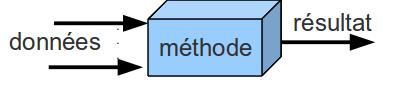
\includegraphics[scale=.6]{../img/methode}
\end{center}
Pour l'utiliser, on doit savoir :
\begin{itemize}
\item Son nom
\item Quoi lui donner
\item Ce qu'elle retourne
\item Mais \emph{pas comment} elle fait
\end{itemize}
\end{frame}

\begin{frame}[fragile]{Appel d'une m�thode}
� partir du code d'une \emph{autre classe} 
  \begin{itemize}
  \item \java|NomClasse.nomM�thode(...)|
  \item \emph{Exemples} :
    \begin{Java}
double racine = Math.sqrt(4.0);
double al�atoire = Math.random();
int nb = -10;
int absolu = Math.abs(nb);
    \end{Java}
  \end{itemize}
Si on est dans la m�me classe
  \begin{itemize}
  \item On indique directement le nom de la m�thode
  \\ \textit{(des exemples suivront)}
  \end{itemize}
\end{frame}

\subsection{D�finition}

\begin{frame}[fragile]{D�finition d'une m�thode}
\begin{Java}
public static typeRetour nomM�thode ( <<param�tre(s) �ventuel(s)>> ) {  
    // code de la m�thode
    return <<r�sultat>>;  // de type : typeRetour
}
\end{Java}
\emph{Exemple} : la moyenne de 2 r�els
\begin{Java}
public static double moyenne ( double nb1, double nb2 ) {  
    double moyenne = (nb1 + nb2) / 2.0;
    return moyenne;
}
\end{Java}
\begin{itemize}
\item Appel possible (si dans la m�me classe)
\begin{Java}
  double cote = moyenne(12.5, 17.5);
\end{Java}
\end{itemize}
\end{frame}

\begin{frame}[fragile]{D�finition d'une m�thode}
\emph{Exemple} : la valeur absolue
\begin{Java}
public static int absolu ( int nb ) {  
    int abs = nb;
    if (nb<0) {
        abs = -nb;
    }
    return abs;
}
\end{Java}
\begin{itemize}
\item Exemples d'appels
\begin{Java}
   int r�sultat = absolu(4);
   int �cart = -10;
   int �cartAbsolu = absolu(�cart);
\end{Java}
\end{itemize}
\end{frame}

\begin{frame}[fragile]{D�finition d'une m�thode}
Si pas de valeur de retour :
\begin{itemize}
\item On indique \java|void|
\item Pas de \java|return|
\end{itemize}
\emph{Exemple} :
\begin{Java}
public static void pr�senter (String nomPgm) {
   System.out.println("Programme "+nomPgm);
} 
\end{Java}
\begin{itemize}
\item Exemple d'appel
\begin{Java}
   pr�senter("moyenne de 2 nombres");
\end{Java}
\end{itemize}
\end{frame}

\begin{frame}[fragile]{D�finition d'une m�thode}
On trouve aussi des m�thodes sans param�tre
\\\emph{Exemple} :
\begin{Java}
public static int lireEntier () {
    Scanner clavier = new Scanner(System.in);
    int nb;
    System.out.println("Entrez un nombre entier!");
    nb = clavier.nextInt();
    return nb;
}
\end{Java}
\begin{itemize}
\item Exemple d'appel
\begin{Java}
   int nb = lireEntier();
\end{Java}
\end{itemize}
\end{frame}

\begin{frame}[fragile]{Commentaire d'une m�thode}
Il est essentiel de commenter chaque m�thode
\begin{itemize}
\item Pour savoir pourquoi et comment l'utiliser
\item Pour la comprendre et ainsi pouvoir la corriger et/ou la modifier
\end{itemize}
\emph{Exemple} : la valeur absolue
\begin{Java}
/**
 * Calcul de la valeur absolue.
 * @param nb le nombre dont on veut la valeur absolue.
 * @return la valeur absolue de <code>nb</code>
 */
public static int absolu ( int nb ) {  
...
}
\end{Java}
\end{frame}

\begin{frame}[fragile]{Commentaire d'une m�thode}
\begin{columns}[T]
\begin{column}{0.48\textwidth}
La documentation suit une notation pr�cise
\begin{itemize}
\item Permet une production automatique de documents d'aide
\item En respectant un style uniforme pour s'y retrouver facilement
\end{itemize}
\end{column}
\begin{column}{0.52\textwidth}
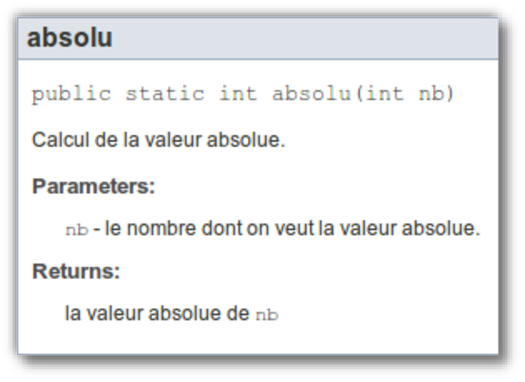
\includegraphics[scale=.7]{../img/module-javadoc}
\end{column}
\end{columns}
\bigskip
Plus de d�tails dans la le�on d�di�e � la documentation du code
\end{frame}

\begin{frame}[fragile]{Un exemple complet}
\begin{Java}[basicstyle=\scriptsize]
package be.heb.esi.lg1.cours;
import java.util.Scanner;

public class MaxEntiers { 

  /**
   * Donne le maximum de 2 nombres.
   * @param nb1 le premier nombre.
   * @param nb2 le deuxi�me nombre.
   * @return la valeur la plus grande entre <code>nb1</code> et <code>nb2</code>
   */
  public static int max ( int nb1, int nb2 ) { 
       int max=0; 
       if (nb1 > nb2) {
           max = nb1;
       } else {
           max = nb2;
       }
       return max;
  }
\end{Java}
\begin{flushright}
{\tiny (\dots)}
\end{flushright}
\end{frame}

\begin{frame}[fragile]{Un exemple complet}
\begin{Java}[basicstyle=\scriptsize]
  /**
   * Lit un nombre entier. 
   * Le nombre est lu sur l'entr�e standard (le clavier).
   * @return le nombre entier lu.
   */
  public static int lireEntier () {
      Scanner clavier = new Scanner(System.in);
      System.out.println("Entrez un nombre entier!");
      return clavier.nextInt();
  }
 
  /**
   * Affiche le maximum de 2 nombres entr�s au clavier.
   * @param args pas utilis�.
   */
  public static void main ( String[] args ) { 
      int max;  // Le max des nombres lus
      int nb1, nb2; // Chacun des nombres lus
      nb1 = lireEntier();
      nb2 = lireEntier();
      max = max(nb1,nb2);
      System.out.println("max = " + max);
  }
}
\end{Java}
\end{frame}

\subsection{Param�tres}

\begin{frame}{Passage de param�tres}
En logique 3 passages de param�tres :
  \begin{itemize}
  \item en entr�e, en sortie, en entr�e-sortie
  \end{itemize} 
\par\bigskip
En Java, uniquement \emph{par valeur}
  \begin{itemize}
  \item = la valeur est copi�e dans le param�tre
  \item $\simeq$ param�tre en entr�e
  \end{itemize} 
\end{frame}

\subsection{Conclusion}

\begin{frame}{Conclusion}
Insistons : Une \emph{m�thode}
\begin{itemize}
\item \emph{fait une et une seule chose}
\item poss�de un \emph{nom explicite}
\item est \emph{fortement document�e}
\end{itemize} 
\end{frame}

% === Cours de Java

\section{Organiser le code}

\leconwithabstract{Dans une application r�elle, la taille des programmes impose une organisation rigoureuse}

\begin{frame}{Le groupement en package}
L'\emph{API} (Application Programming Interface) d�signe la biblioth�que standard Java
\begin{itemize}
\item Elle contient des \emph{milliers} de classes
\item Elles sont regroup�es en \emph{package}
\end{itemize}
\begin{center}
  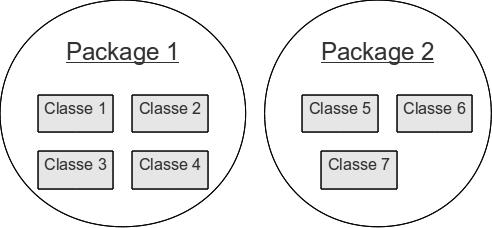
\includegraphics[scale=.6]{../img/package}
\end{center}
\end{frame}

\begin{frame}{La notion de package}
Un \emph{package}
\begin{itemize}
\item Regroupe les classes li�es
\item Permet l'unicit� des noms de classe
  \begin{itemize}
    \item nom complet / qualifi�: {\small \java|monPackage.MaClasse|}
  \end{itemize} 
\end{itemize} 
\bigskip
Nom d'un package
  \begin{itemize}
    \item identifieurs s�par�s par des points \java|.|
    \item tout en minuscules
    \item adresse internet invers�e (unicit�)
    \item ex: {\small \java|be.heb.esi.java1|}, {\small \java|org.apache.struts.action|}
  \end{itemize} 
\end{frame}

\begin{frame}[fragile]{Utilisation}
Pour utiliser une classe 
\begin{itemize}
\item mettre le nom \emph{qualifi�} (complet)
\begin{Java}
  java.util.Calendar now = java.util.Calendar.getInstance();
\end{Java}
\item ou utiliser \java{import} qui cr�e un raccourci
\begin{Java}[basicstyle=\scriptsize]
  import java.util.Calendar;
  public Test {
  ...
    Calendar now = Calendar.getInstance();
  ...
  }
\end{Java}
\item Cas particulier : le package \java|java.lang| est import� implicitement
  \begin{itemize}
  \item Exemple : on peut tout de suite �crire
  \begin{Java}
  double racine = Math.sqrt(1.21);
  \end{Java}
  \end{itemize}
\end{itemize}
\end{frame}

\begin{frame}{Utilisation}
Comment savoir comment utiliser les classes et m�thodes ? En lisant la \emph{javadoc}
\begin{center}
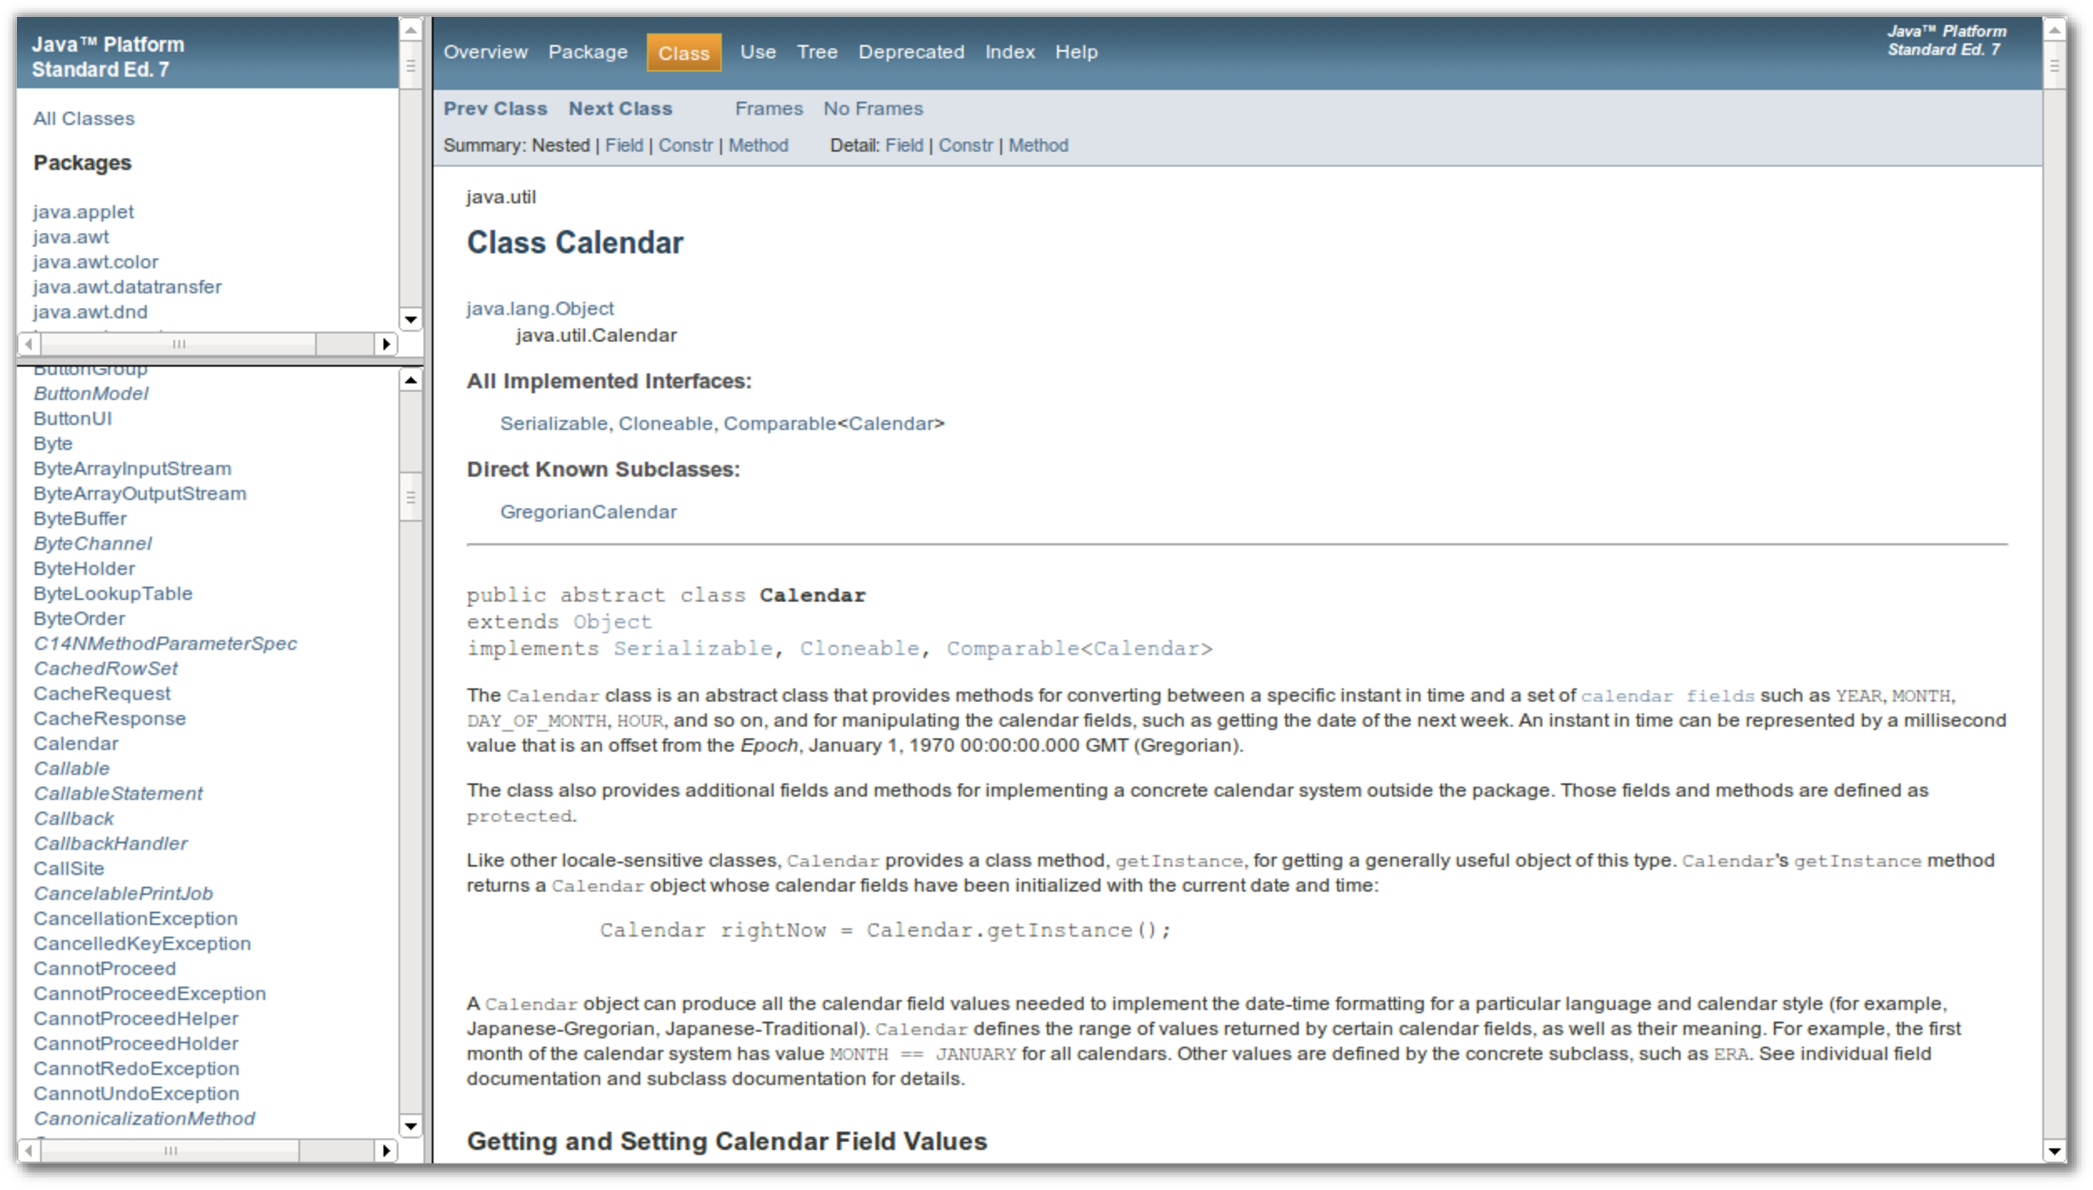
\includegraphics[scale=.28]{../img/api}
\\ \scriptsize{\textit{(http://download.oracle.com/javase/7/docs/api/)}}
\end{center}
\end{frame}

\begin{frame}{Utilisation}
On peut y lire le nom du package 
\begin{center}
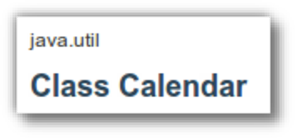
\includegraphics[scale=.6]{../img/api-package}
\end{center}
et la description de la m�thode
\begin{center}
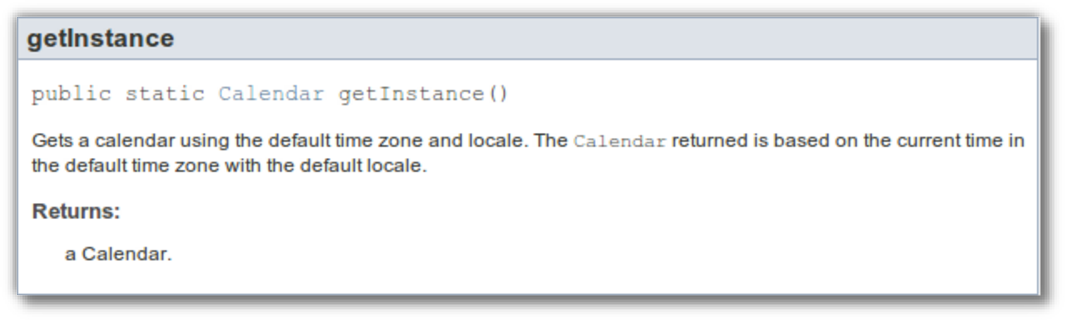
\includegraphics[scale=.6]{../img/api-methode}
\\{\small \textit{On verra comment produire une \emph{javadoc} similaire pour son code}}
\end{center}
\end{frame}

\begin{frame}[fragile]{Cr�er ses packages}
Pour placer une classe dans un package, la commande est \java|package nom_package;|
  \begin{itemize}
  \item Doit �tre la \emph{premi�re instruction} du fichier 
  \item Exemple :
\begin{Java}
package be.heb.esi.java1;
public class Test { 
  // Nom complet : be.heb.esi.java1.Test
}
\end{Java}
  \end{itemize}
\end{frame}

\begin{frame}[fragile]{Cr�er ses packages}
Qu'est-ce qui va changer en pratique ?
\begin{itemize}
\item La compilation ne change pas : 
 \begin{Java}
 javac NomClasse.java
 \end{Java}
\item L'ex�cution change : 
 \begin{Java}
 java nomPackage.NomClasse
 \end{Java}
\item Contraintes sur l'endroit o� placer le \emph{bytecode}
  \begin{itemize}
  \item Li� � la notion de \emph{CLASSPATH} 
  \item Sera d�taill� au laboratoire
  \end{itemize}
\end{itemize}
\end{frame}

\begin{frame}{R�utiliser du code}
Si on doit coder quelque chose, c'est \emph{peut-�tre d�j� fait}
\begin{itemize}
\item $\Longrightarrow$ autant le r�utiliser
  \begin{itemize}
  \item Gain de temps
  \item Probablement mieux �crit
  \end{itemize}
\item Importance de \emph{connaitre l'API}
\\(en tout cas les classes principales)
\end{itemize}
\end{frame}



% === Cours de Java
% === Chapitre : Survol 

\section{Les boucles (survol)}

\leconwithabstract{Nous voyons comment traduire les algorithmes contenant des boucles que vous �crivez au cours de Logique}

\begin{frame}[fragile]{Instructions r�p�titives}
Le \emph{Tant que} : 
\begin{Java}
  while ( condition ) {
    instructions
  }
\end{Java} 
\bigskip
\emph{Exemple} :
\begin{Java}
  int puissance = 1;
  while ( puissance < 1000 ) {
    System.out.println(puissance);
    puissance = 2 * puissance;
  }
\end{Java}
\end{frame}

\begin{frame}[fragile]{Exemple} 
\begin{Java}
import java.util.Scanner;
public class Exemple {
  /**
   * Affiche la somme d'entiers positifs entr�s au clavier.
   * S'arr�te d�s qu'une valeur nulle ou n�gative est donn�e.
   * @param args non utilis�
   */
  public static void main(String[] args) {
      Scanner clavier = new Scanner(System.in);
      int nb;
      int somme = 0;
      nb = clavier.nextInt();
      while ( nb > 0 ) {
         somme = somme + nb;
         nb = clavier.nextInt();
      }
      System.out.println(somme);
  }
}
\end{Java}
\end{frame}

\begin{frame}[fragile]{Instructions r�p�titives}
Le \emph{Pour} : 
\begin{Java}
  for ( int i=d�but; i<=fin; i=i+pas ) {
    instructions
  }
\end{Java} 
\bigskip
\emph{Exemple} :
\begin{Java}
  for ( int i=1; i<=10; i=i+1 ) {
    System.out.println(i);
  }
\end{Java}
\end{frame}

\begin{frame}[fragile]{Exemple} 
\begin{Java}
public class Exemple {
  /**
   * Affiche la somme des nombres pairs entre 2 et 100.
   * @param args non utilis�
   */
  public static void main(String[] args) {
      int somme;

      somme = 0;
      for ( int i=2; i<=100; i=i+2 ) {
         somme = somme + i;
      }
      System.out.println(somme);
  }
}
\end{Java}
\end{frame}

\begin{frame}[fragile]{Exemple} 
\begin{Java}
public class Exemple {
  /**
   * Affiche un compte � rebours � partir de 10.
   * @param args non utilis�
   */
  public static void main(String[] args) {

      for ( int i=10; i>=1; i=i-1 ) {
         System.out.println(i);
      }
      System.out.println("Partez !");
  }
}
\end{Java}
\end{frame}

\begin{frame}[fragile]{Instructions r�p�titives}
\java|i++| est un raccourci pour \java|i=i+1|
\\\bigskip
\emph{Exemple} :
\begin{Java}
  for ( int i=1; i<=n; i++ ) {
    System.out.println(i);
  }
\end{Java} 
\end{frame}

\begin{frame}[fragile]{�tude de cas} 
\emph{Objectif} : lecture d'une donn�e enti�re positive
\begin{itemize}
\item \emph{�tape 1} : lire un entier
\end{itemize}
\begin{Java}
/**
  * Lit un entier au clavier.
  * Les valeurs non enti�res sont pass�es.
  * @return l'entier lu.
  */
public static int lireEntier() {
    Scanner clavier = new Scanner(System.in);
    int nb;
    // Tant que ce n'est pas un entier au clavier
    while ( !clavier.hasNextInt() ) {
        clavier.next(); // le lire, le passer
    }
    nb = clavier.nextInt();
    return nb;
}
\end{Java}
\end{frame}

\begin{frame}[fragile]{�tude de cas} 
\begin{itemize}
\item \emph{�tape 2} : lire un entier positif
\end{itemize}
\begin{Java}
/**
  * Lit un entier au clavier.
  * Les valeurs non enti�res, nulles ou n�gatives sont pass�es.
  * @return l'entier lu.
  */
public static int lirePositif() {
    int nb;
    nb = lireEntier();
    while (nb<=0) {
      nb = lireEntier();
    }
    return nb;
}
\end{Java}
\end{frame}




% === Cours de Java
\section{�crire du code robuste}

\leconwithtoc

\subsection{Motivation}

\begin{frame}{Motivation}
Un programme ne tourne pas dans un monde id�al
\\\bigskip
Il doit pouvoir \emph{r�sister aux d�faillances} de l'environnement
  \begin{itemize}
  \item On tente d'ouvrir un fichier qui n'existe pas
  \item L'utilisateur entre des donn�es incorrectes
  \item \dots
  \end{itemize}
\end{frame}

\subsection{G�rer les erreurs}

\begin{frame}[fragile]{La gestion des erreurs}
\emph{Exemple} :
\begin{Java}
import java.util.Scanner;
public class Affiche {
  /**
   * Affiche un nombre entier lu au clavier.
   * @param args non utilis�
   */
  public static void main(String[] args) {
      Scanner clavier = new Scanner(System.in);
      int nb;
 
      nb = clavier.nextInt();
      System.out.println(nb);
  }
}
\end{Java}
\begin{itemize}
\item � priori tout va bien !
\end{itemize}
\end{frame}

\begin{frame}[fragile]{La gestion des erreurs}
Et si l'utilisateur entre une lettre ?
\vspace{-1ex}
\begin{center}
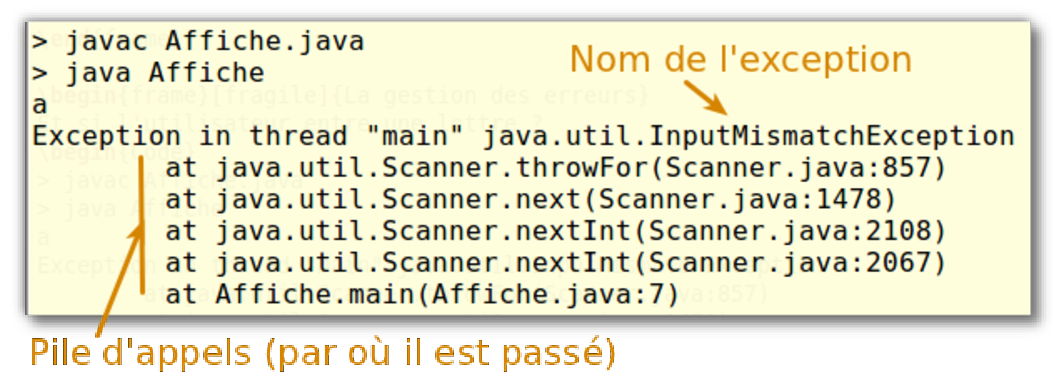
\includegraphics[scale=.65]{../img/erreur1}
\end{center}
\vspace{-1ex}
%\begin{Code}
%> javac Affiche.java
%> java Affiche
%a
%Exception in thread "main" java.util.InputMismatchException
%	at java.util.Scanner.throwFor(Scanner.java:857)
%	at java.util.Scanner.next(Scanner.java:1478)
%	at java.util.Scanner.nextInt(Scanner.java:2108)
%	at java.util.Scanner.nextInt(Scanner.java:2067)
%	at Affiche.main(Affiche.java:7)
%\end{Code}
  \begin{itemize}
  \item Une \emph{exception} est g�n�r�e
  \item Le programme s'\emph{arr�te brutalement} et affiche un message d'erreur
  \end{itemize}
\end{frame}

\begin{frame}{La gestion des erreurs}
2 inconv�nients majeurs
  \begin{itemize}
  \item Le message d'erreur est tr�s utile pour le d�veloppeur mais pas pour l'utilisateur
  \item L'arr�t du programme est rarement le comportement souhait�
  \end{itemize}
\bigskip
On aimerait pouvoir \emph{g�rer} le probl�me
  \begin{itemize}
  \item Au mieux, le r�gler
  \item Au pire, afficher un message plus clair pour l'utilisateur
  \end{itemize}
\end{frame}

\begin{frame}[fragile]{La gestion des erreurs}
Possible gr�ce � l'instruction \java|try catch|
  \begin{itemize}
  \item \java{try} : contient les instructions qui \emph{peuvent mal se passer}
  \item \java{catch} : contient le code qui est \emph{en charge} de g�rer le probl�me
  \end{itemize}
\bigskip
Quand un probl�me se pr�sente dans le \java{try}
  \begin{itemize}
  \item Le code du \java{try} est interrompu
  \item Le code du \java{catch} est ex�cut�
  \item Ensuite, on continue apr�s le \java{try-catch} 
  \end{itemize}
\end{frame}

\begin{frame}[fragile]{La gestion des erreurs}
\emph{Exemple} : on affiche un message plus clair
\begin{Java}[basicstyle=\scriptsize]
package be.heb.esi.lgj1;
import java.util.Scanner;
public class Affiche {
  /**
   * Affiche l'entier lu au clavier ou un message si ce n'est pas un entier.
   * @param args inutilis�.
   */
  public static void main(String[] args) {
      Scanner clavier = new Scanner(System.in);
      int nb;
      try { 
        nb = clavier.nextInt();
        System.out.println(nb);
      }
      catch(Exception e) { 
        System.out.println("Ce n'est pas un entier!");
      }
  }
}
\end{Java}
\vspace{-4ex}
\hspace{3ex}
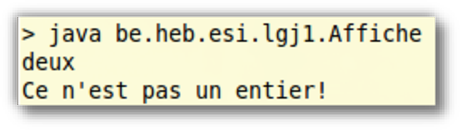
\includegraphics[scale=.65]{../img/throw}
\end{frame}

\subsection{Confiner les probl�mes}

\begin{frame}{Confiner les probl�mes - Motivation}
Imaginons la situation suivante :
\begin{itemize}
\item Un programme demande un entier � l'utilisateur
\item Il doit �tre positif
\item L'utilisateur entre un nombre n�gatif
\item Le programme ne le v�rifie pas tout de suite
\end{itemize}
\end{frame}

\begin{frame}{Confiner les probl�mes - Motivation}
On aura un probl�me :
\begin{itemize}
\item Un plantage
\item Un r�sultat erron�
\item Un effet ind�sir� (perte de donn�es, \dots)
\end{itemize}
\medskip
Mais le probl�me va survenir :
\begin{itemize}
\item Plus tard dans le temps
\item Plus loin dans le code
\end{itemize}
\medskip
$\Longrightarrow$ \emph{Difficile} � comprendre et \emph{corriger}
\end{frame}

\begin{frame}{Confiner les probl�mes}
Besoin de \emph{confiner} les probl�mes
  \begin{itemize}
  \item Un probl�me est \emph{d�tect� rapidement} avant qu'il ne se propage dans le reste du code
  \end{itemize}
\bigskip
Cas pratique : v�rifier les \emph{param�tres}
  \begin{itemize}
  \item Si une contrainte est associ�e � un param�tre
    \begin{itemize}
    \item Le v�rifier en d�but de m�thode
    \item Que faire si pas valide ?
    \end{itemize}
  \end{itemize}
\end{frame}

\begin{frame}[fragile]{Confiner les probl�mes}
Nous avons appris � attraper une exception.
\par
On peut aussi en cr�er une
\begin{Java}[basicstyle=\scriptsize]
  /**
   * Calcule la racine carr�e d'un nombre.
   * @param nb le nombre dont on veut la racine car�e.
   * @return la racine carr�e de <code>nb<\code>.
   * @throws IllegalArgumentException si <code>nb</code> est n�gatif.
   */
  public static double racineCarr�e(double nb) {
    if (nb<0) {
      throw new IllegalArgumentException("nb doit �tre positif!");
    }
    // Traitement normal. On est s�r que le param�tre est OK.
  }
\end{Java}
\begin{itemize}
\item On dit qu'on \emph{lance} une exception
\\(ici de type \java|IllegalArgumentException|)
\item Pourra �tre attrap�e via un \java{catch}
\end{itemize}
\end{frame}

\begin{frame}[fragile]{Confiner les probl�mes}
\emph{Exemple}
\begin{Java}
  try {
    System.out.println( racineCarr�e( val ) );
  } catch (Exception ex) {
    System.out.println( "Calcul impossible !" );
  }
\end{Java}
\bigskip
On peut aussi pr�ciser qu'on n'attrape \emph{que} les \java|IllegalArgumentException|
\begin{Java}
  try {
    System.out.println( racineCarr�e( val ) );
  } catch (IllegalArgumentException ex) {
    System.out.println( "Calcul impossible !" );
  }
\end{Java}
\end{frame}

% === Cours de Java
% === Chapitre : Les donn�es

\section{Les types et les litt�raux}

\leconwithtoc

\subsection{Un langage typ�}

\begin{frame}{Les types}
\emph{Toute donn�e a un type}
  \begin{itemize}
  \item Coh�rence s�mantique
  \item Allocation m�moire adapt�e
  \end{itemize}  
\bigskip
Quels types ?
\begin{itemize}
  \item \emph{primitifs pr�d�finis} : 
\begin{itemize}
\item entier, r�el, bool�en (logique)
\end{itemize}
  \item \emph{r�f�rences pr�d�finis} :
\begin{itemize}
\item tableaux, String, \dots
\end{itemize}
  \item \emph{r�f�rences d�finis par le programmeur}
  \end{itemize}
\end{frame}

\begin{frame}[fragile]{Les types primitifs}
\vspace{-25pt}
\begin{center}
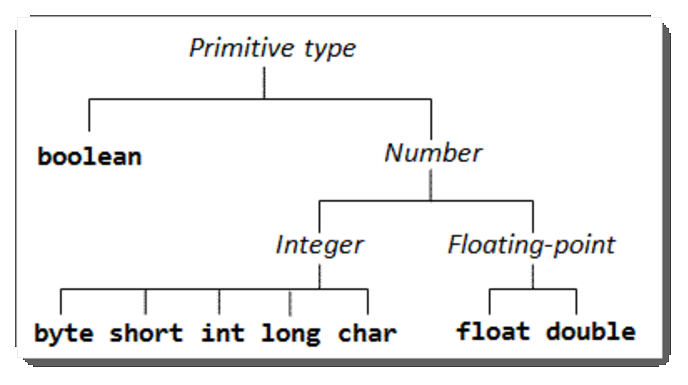
\includegraphics[scale=.65]{../img/primitifs}
\\\tiny{source : http://www3.ntu.edu.sg/home/ehchua/programming/java/J2\_Basics.html}
\end{center}
\vspace{-25pt}
\begin{columns}[T]
\begin{column}{0.5\textwidth}
\begin{grammaire}
\nterm{PrimitiveType} : one of
    \nterm{NumericType}  \term{boolean}

\nterm{NumericType} : one of
    \nterm{IntegralType}  \nterm{FloatingPointType}
\end{grammaire}
\end{column}
\begin{column}{0.4\textwidth}
\begin{grammaire}
\nterm{IntegralType} : one of
    \term{byte}  \term{short}  \term{int}  \term{long}  \term{char}

\nterm{FloatingPointType} : one of
    \term{float}  \term{double}
\end{grammaire}
\end{column}
\end{columns}
\end{frame}

\subsection{Les types entiers}

\begin{frame}[fragile]{Les types num�riques entiers}
\java|byte|, \java|short|, \java|int| et \java|long| 
(\java|char| sera vu � part) :
\begin{itemize}
\item Nombres sign�s (en compl�ment � 2)
\item Cod�s sur 8-bit, 16-bit, 32-bit et 64-bit
\item Comprennent donc les valeurs 
  \begin{itemize}
  \item -128 � 127
  \item -32768 � 32767
  \item -2147483648 � 2147483647
  \item -9223372036854775808 � 9223372036854775807
  \end{itemize} 
\item \emph{Mod�lisation} de la notion math�matique d'entier
  \begin{itemize}
  \item Capacit� limit�e 
  \item permet de repr�senter un intervalle fini de $\mathbb{Z}$
  \item \emph{\textit{out of range}} possible
  \end{itemize} 
\end{itemize}
\end{frame}

\begin{frame}[fragile]{Les litt�raux entiers}
\emph{\textit{Litt�ral}} : repr�sentation d'une valeur
\\\smallskip
Pour les entiers, diff�rents formats sont possibles
\begin{center}
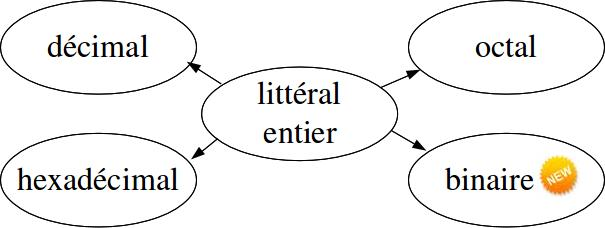
\includegraphics[scale=.35]{../img/java-data-entier}
\end{center} 
\begin{grammaire}
\nterm{IntegerLiteral} : one of
       \nterm{DecimalIntegerLiteral}    \nterm{HexIntegerLiteral}  
       \nterm{OctalIntegerLiteral}        \nterm{BinaryIntegerLiteral}
\end{grammaire}
\end{frame}

\begin{frame}[fragile]{Les litt�raux entiers}
Un \emph{\nterm{DecimalNumeral}} (num�rique d�cimal)  
\vspace{-10pt}
\begin{columns}[T]
\begin{column}{0.6\textwidth}
\begin{grammaire}[fontsize=\footnotesize]
\nterm{DecimalIntegerLiteral} :
     \nterm{DecimalNumeral} \nterm{IntegerTypeSuffix}\opt
\end{grammaire}
\end{column}
\begin{column}{0.4\textwidth}
\begin{grammaire}[fontsize=\footnotesize]
\nterm{IntegerTypeSuffix} : one of \term{l} \term{L}
\end{grammaire}
\end{column}
\end{columns}
  \begin{itemize}
  \item \nterm{DecimalNumeral} : suite de chiffres
  \item \java|_| permis pour la lisibilit� 
\includegraphics[scale=.5]{../img/java7.jpeg} 
  \item Le suffixe (\java|l| ou \java|L|) : distingue un \java|int| d'un \java|long|
  \item Pas de \java|byte| ou \java|short| ? �crire un \java|int|
  \item Pas de \emph{litt�ral n�gatif} ? Utiliser le \java|-|
  \item Exemples corrects : \java|0   1275   1_421   23L| 
  \item Exemples incorrects : \java|12.3   1 000   1,000   1.0| 
  \end{itemize} 
\end{frame}

\begin{frame}[fragile]{Les litt�raux entiers}
\emph{Octal}
  \begin{itemize}
  \item pr�c�d� de \java|0|
  \item chiffres de 0 � 7
  \end{itemize} 
\emph{H�xad�cimal}
  \begin{itemize}
  \item pr�c�d� de \java|0x| ou \java|0X|
  \item chiffres + a,b,c,d,e,f (minuscules/majuscules)
  \end{itemize} 
\emph{Binaire}
  \begin{itemize}
  \item pr�c�d� de \java|0b| ou \java|0B|
  \item chiffres 0 et 1
  \end{itemize} 
\end{frame}

\begin{frame}[fragile]{Les litt�raux entiers}
\emph{Exemple} : Quelques litt�raux corrects pour la quantit� 100 de type \java|int| 
\begin{itemize}
\item \java|100|
\item \java|1_0_0|
\item \java|0144|
\item \java|01_44|
\item \java|0x64|
\item \java|0b110_0100|
\end{itemize} 
\end{frame}

\begin{frame}[fragile]{Le type num�rique caract�re}
\java|char|
\begin{itemize}
\item Caract�re Unicode
\item Entier non sign� sur 16 bits
\item Assimil� � un entier (on peut faire des calculs !)
\item Plusieurs notations  
\begin{grammaire}[commandchars=|()]
|nterm(CharacterLiteral) :
    |term(') |nterm(SingleCharacter) |term(')
    |term(') |nterm(EscapeSequence) |term(')
\end{grammaire} 
\item La plus simple : le \emph{caract�re entre \textit{single quote}} 
\begin{grammaire}[commandchars=|()]
|nterm(SingleCharacter) :
    any character but not |term(') or |nterm(\) or |nterm(LineTerminator)
\end{grammaire} 
\end{itemize}
\end{frame}

\begin{frame}[fragile]{Les litt�raux caract�res}
Notations sp�ciales avec les s�quences d'�chappement (\textit{Escape Sequence})
\begin{itemize}
\item Pour les caract�res non repr�sentables simplement
\\\medskip
\begin{tabular}{r|llr|llr|l}
\java|\n| & line feed       & \hspace{0.3cm} & \java|\t| & tabulation & \hspace{0.3cm} & \java|\'| & \code|'| \\
\java|\r| & carriage return & \hspace{0.3cm} & \java|\b| & backspace  & \hspace{0.3cm} & \java|\"| & \code|"| \\
          &                 & \hspace{0.3cm} &           &            & \hspace{0.3cm} & \java|\\| & \code|\| \\
\end{tabular}
\medskip
\begin{itemize}
\item Exemples : \java|'\n'| ,\java|'\\'| ,\java|'\''|
\end{itemize}
\item Pour utiliser le code Unicode
\begin{itemize}
\item Exemples : 
  \begin{itemize}
  \item \java|'\u0F40'| pour le \textit{KA} tib�tain 
  \item \java|'\u17E0'| pour le chiffre 0 Khmer 
  \end{itemize}
\end{itemize}
\end{itemize}
\end{frame}

\subsection{Les types flottants}

\begin{frame}[fragile]{Les types � virgule flottante}
\java|float|, \java|double| 
\begin{itemize}
\item Respectent la norme IEEE754
\item Cod�s sur (respectivement) 32-bit, et 64-bit
\item On utilisera plus souvent le type \java|double|
\item \emph{Mod�lisation} de la notion math�matique
  \begin{itemize}
  \item Capacit� limit�e (\emph{\textit{out of range}} possible) 
  \item Pr�cision limit�e
    \begin{itemize}
    \item $\longrightarrow$ \emph{impr�cision} lors d'un calcul
    \item ex : $10^{-30}$ est repr�sentable et pourtant \\$(1+10^{-30})-1$ donnera $0$ et pas $10^{-30}$
    \end{itemize}
  \end{itemize} 
\end{itemize}
\end{frame}

\begin{frame}[fragile]{Les litt�raux � virgule flottante}
Notation assez souple
\begin{grammaire}
\nterm{FloatingPointLiteral} :
      \nterm{Digits} \term{.} \nterm{Digits}\opt \nterm{ExponentPart}\opt \nterm{FloatTypeSuffix}\opt
      \term{.} \nterm{Digits} \nterm{ExponentPart}\opt \nterm{FloatTypeSuffix}\opt
      \nterm{Digits} \nterm{ExponentPart} \nterm{FloatTypeSuffix}\opt
      \nterm{Digits} \nterm{ExponentPart}\opt \nterm{FloatTypeSuffix}

\nterm{ExponentPart} :
      \term{e} \nterm{signedInteger}
      \term{E} \nterm{signedInteger}

\nterm{FloatTypeSuffix} : one of
      \term{f} \term{F} \term{d} \term{D}
\end{grammaire}
\end{frame}

\begin{frame}[fragile]{Les litt�raux � virgule flottante}
\begin{small}
\begin{tabular}{|c|c|c|c|c|c|}
\hline
partie enti�re & . & partie d�cimale & E & exposant & suffixe \\
\hline
\end{tabular}
\end{small}
\smallskip
\begin{itemize}
\item 4 parties optionnelles (mais pas ensemble)
\begin{itemize}
\item Cela doit rester sens�
\item On ne peut pas le confondre avec un entier
\end{itemize}
\item En l'absence de suffixe : un double
\item Exemples : \java|1.2E3|, \java|1.F|, \java|.1|, \java|1e-2d|, \java|1f|
\item Contre-exemples : \java|1|, \java|.E1|, \java|E1|
\end{itemize}
\end{frame}

\subsection{Les bool�ens}

\begin{frame}{Le type bool�en}
\java|boolean|
\begin{itemize}
\item Appel� aussi \emph{logique}
\item 2 valeurs : \java|true| (vrai) et \java|false| (faux)
\end{itemize}
\end{frame}

\subsection{La chaine de caract�res}

\begin{frame}[fragile]{La chaine de caract�res}
\java|String|
\begin{grammaire}[commandchars=|()]
|nterm(StringLiteral) :
      |term(") |nterm(StringCharacters)|opt |term(")
|nterm(StringCharacters) :
      |nterm(StringCharacter)
      |nterm(StringCharacters) |nterm(StringCharacter)
|nterm(StringCharacter) :
      |nterm(InputCharacter) but not |term(") or |term(\)
      |nterm(EscapeSequence)
|nterm(InputCharacter) :
      |nterm(UnicodeInputCharacter) but not |term(CR) or |term(LF)
\end{grammaire}
\begin{itemize}
\item Exemples de \java|String| :
\begin{itemize}
\item \java|"Bonjour "|
\item \java|"'Un peu de tout' : \"\n\\"|
\end{itemize} 
\item Attention : \java|char| $\neq$ \java|String|
\end{itemize}
\end{frame}


% === Cours de Java

\section{Les tableaux (survol)}

\leconwithtoc

\subsection{Pr�sentation}

\begin{frame}{Avertissement}
\begin{center}
Nous pr�sentons ici une \emph{vue} tr�s \emph{simplifi�e} 
\\des tableaux en Java afin de \emph{coller} 
\\� votre cours de \emph{logique}.
\bigskip
\\Nous aurons l'occasion d'�tre plus pr�cis 
\\lors d'une prochaine le�on.
\end{center}
\end{frame}

\begin{frame}[fragile]{Pr�sentation}
N�cessit� de manipuler \emph{plusieurs variables similaires}
\begin{itemize}
\item \emph{Ex}: plusieurs cotes, plusieurs temp�ratures
\item Acc�s � un des �l�ments via un \emph{indice} (\textit{position})
\end{itemize}
  \begin{center}
  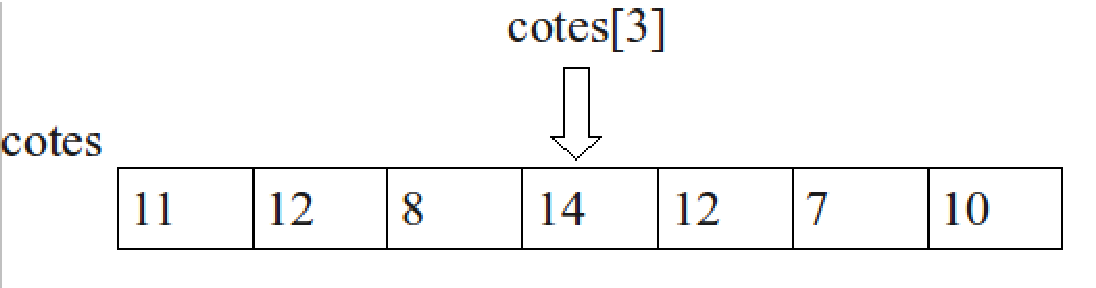
\includegraphics[scale=.35]{../img/tab-pres}
  \end{center}
\pause
Pourquoi pas plusieurs variables ?
  \begin{itemize}
  \item �criture \emph{compacte} et qui s'\emph{adapte} � la taille
  \item \emph{Ex} : En logique, si \java|tab| est un tableau de $N$ entiers
        \begin{Java}
  pour i de 1 � N faire
     �crire tab[i]
  fin pour
        \end{Java}
  \end{itemize}
\end{frame}

\subsection{Type / D�claration / Cr�ation}

\begin{frame}[fragile]{Type et d�claration}
El�ments de type \java|T| $\Rightarrow$ type du tableau = \java|T[]|
\\\emph{Exemples}
    \begin{itemize}
    \item \java|int[]| est le type \textit{tableau d'entiers}
    \item \java|String[]| est le type \textit{tableau de chaines de caract�res}
    \end{itemize}
\medskip\pause
En \sigle{Java} : uniquement des tableaux \emph{dynamiques}
    \begin{itemize}
    \item La taille ne fait pas partie du type
    \item D�claration et cr�ation sont s�par�es
    \end{itemize}
\medskip\pause
La d�claration suit la syntaxe habituelle
\\\emph{Exemples}
    \begin{Java}
    int[] cotes;
    String[] noms;
    \end{Java}
\end{frame}

\begin{frame}[fragile]{Cr�ation}
Il faut encore \emph{cr�er} le tableau (via le mot cl� \java|new|)
\\\emph{Exemple} :
    \begin{Java}
    int[] entiers;
    entiers = new int[3];
    \end{Java}
    \vspace{-10pt}
  \begin{center}
  entiers \begin{tabular}{|c|c|c|}\hline  &   &  \\\hline\end{tabular}
  (espace pour 3 entiers)
  \end{center}
    \pause
On peut aussi combiner d�claration/cr�ation
  \\\emph{Exemple} :
    \begin{itemize}
    \item \java|int[] entiers = new int[3];|
    \end{itemize}
\medskip\pause
�l�ments initialis�s � \java|0| (num�riques) ou \java|false| (bool�ens)
\end{frame}

\begin{frame}[fragile]{Cr�ation}
On peut aussi cr�er le tableau en \emph{donnant ses valeurs}
  \begin{itemize}
  \item Dans ce cas, on ne sp�cifie pas la taille \\(elle est d�duite)
  \item \emph{Exemple} :
    \begin{Java}
    int[] entiers = {4,5,6};
    \end{Java}
  \medskip
  entiers \begin{tabular}{|c|c|c|}\hline 4 & 5  & 6 \\\hline\end{tabular}
  \end{itemize}
\end{frame}

\subsection{Acc�s}

\begin{frame}[fragile]{Acc�s aux �l�ments}
\emph{D�finition} : taille = Nombre d'�l�ments
\\\medskip
En \sigle{Java} on ne choisit pas l'indice de d�part : toujours 0
  \begin{itemize}
  \item $\longrightarrow$ Indices de \emph{0 � taille du tableau - 1}
  \item Exemple :
    \begin{Java}
    int[] entiers = {7,14,0};
    int entier = entiers[2]; // entier vaut 0
    entiers[1] = 85;
    entier = entiers[entier+1]; //entier vaut 85
    \end{Java}
  \end{itemize}
\end{frame}

\begin{frame}[fragile]{Acc�s aux �l�ments}
  \emph{Exemple} : Initialisation des composants d'un tableau d'entiers � la valeur de leur indice
  \begin{Java}
  package be.heb.esi.lg1.tutorials.tableaux;

  public class InitialisationTableau {
     public static void main(String[] args) {
        int[] entiers = new int[10];
        for(int i = 0; i < 10; i++) {
           entiers[i] = i;
        }
     }
  }
  \end{Java}
\end{frame}

\subsection{Taille}

\begin{frame}[fragile]{Taille}
En \sigle{Java} : tout tableau connait sa \emph{taille}
  \begin{itemize}
  \item Via \java|nomTableau.length|
  \item \emph{Exemple} :
    \begin{Java}
   int[] entiers = {4,5,6};
   int taille = entiers.length;
   System.out.println(taille); // �crit 3
    \end{Java}
  \item Permet d'�crire un code qui s'adapte mieux aux changements
  \end{itemize}
\end{frame}

\begin{frame}[fragile]{Taille}
  \emph{Exemple} : Parcours des composants d'un tableau d'entiers suivant l'ordre ascendant des indices
  \begin{Java}
  package be.heb.esi.lg1.tutorials.tableaux;

  public class SimpleParcoursAscendant {
     public static void main(String[] args){
        int[] entiers = {1,2,3,4,5,6,7,8,9,10};
        for(int i = 0; i < entiers.length; i = i + 1) {
           System.out.println(entiers[i]);
        }
     }
  }
  \end{Java}
\end{frame}

\begin{frame}[fragile]{Taille}
  \emph{Exemple} : Parcours des composants d'un tableau d'entiers suivant l'ordre descendant des indices
  \begin{Java}
  package be.heb.esi.lg1.tutorials.tableaux;

  public class SimpleParcoursDescendant {
     public static void main(String[] args){
        int[] entiers = {1,2,3,4,5,6,7,8,9,10};
        for(int i = entiers.length - 1; i >= 0; i = i-1) {
           System.out.println(entiers[i]);
        }
     }
  }
  \end{Java}
\end{frame}

\subsection{Tableau et m�thode}

\begin{frame}[fragile]{Tableau et m�thode}
Un tableau peut �tre un param�tre d'une m�thode.
\\\emph{Exemple} : Afficher un tableau 
\begin{Java}
   public static void afficher( int[] entiers ) {
      for(int i = 0; i<entiers.length; i++) {
         System.out.println(entiers[i]);
      }
   }
\end{Java}
\begin{itemize}
  \item L'appel pourrait �tre
  \begin{Java}
  int[] cotes = {12,8,10,14,9};
  afficher( cotes );
  \end{Java}
\end{itemize}
\end{frame}

\begin{frame}[fragile]{Tableau et m�thode}
En \sigle{Java} : passage de param�tres par \emph{valeur}
\begin{itemize}
\item normalement $\equiv$ param�tre en entr�e
\item pour un tableau $\equiv$ param�tre en \emph{entr�e-sortie}
\end{itemize}
\medskip
{\small (li� � la r�pr�sentation m�moire que nous verrons plus tard)}
  \emph{Exemple} : Remplir un tableau 
  \begin{Java}
   public static void remplir( int[] entiers, int val ) {
      for(int i = 0; i<entiers.length; i++) {
         entiers[i] = val;
      }
   }
  \end{Java}
  \begin{itemize}
  \item L'appel pourrait �tre
  \begin{Java}
  int[] cotes = new int[16]; // Ne pas oublier de le cr�er
  remplir( cotes, 20 );
  \end{Java}
  \end{itemize}
\end{frame}

\begin{frame}[fragile]{Tableau et m�thode}
  Un tableau peut �tre une valeur de retour
  \\\emph{Exemple} : Cr�er un tableau avec valeur
  \begin{Java}
   public static int[] cr�er( int taille, int val ) {
      int[] entiers = new int[taille];
      for(int i = 0; i<taille; i++) {
         entiers[i] = val;
      }
      return entiers;
   }
  \end{Java}
  \begin{itemize}
  \item L'appel pourrait �tre
  \begin{Java}
  int[] cotes = cr�er(16, 20);
  \end{Java}
  \end{itemize}
\end{frame}

\subsection{Plusieurs dimensions}

\begin{frame}[fragile]{Tableaux � plusieurs dimensions}
Pour indiquer plusieurs dimensions, on multiple les \java{[]}
\\\emph{Exemple} :
\begin{Java}
    int[][] entierss = new int[3][4];
    for( int i=0; i<3; i++) {
      for( int j=0; j<4; j++) {
          entierss[i][j] = i*j*(i+j);
      }
    } 
\end{Java}
\end{frame}

\begin{frame}[fragile]{Tableaux � plusieurs dimensions}
On peut demander le nb de colonnes comme le nb de lignes
\\\emph{Exemple} : afficher un tableau re�u en param�tre
\begin{Java}
public static void afficher(int[][] entierss) {
    for( int i=0; i<entierss.length; i++) {
        for( int j=0; j<entierss[0].length; j++) {
            System.out.print(entierss[i][j] + " ");
        }
        System.out.println();
    }
} 
\end{Java}
\end{frame}

\subsection{Erreurs fr�quentes}

\begin{frame}[fragile]{Erreurs fr�quentes}
Lorsque vous manipulerez des tableaux vous pourrez tomber sur ces exceptions
\begin{itemize}
\item \java|NullPointerException| : si vous essayez d'acc�der � un �l�ment d'un tableau qui n'a pas �t� cr��
\\(le tableau vaut \java|null| dans ce cas)
\item \java|ArrayIndexOutOfBoundsException| : si vous donnez un indice qui n'existe pas (ex: \java|tab[10]| quand il n'y a que 10 �l�ments dans le tableau)
\end{itemize}
\end{frame}


% === Cours de Java
% === Chapitre : Javadoc
\section{La documentation Java}

\leconwithtocquote{\og  It's not a bug - it's an undocumented feature. \fg
\\Author Unknown}

\subsection{Motivation}

\begin{frame}{Motivation}
Documenter son code
\begin{itemize}
\item Pour qui ?
\begin{itemize}
\item Le programmeur qui va \emph{utiliser} le code
\item Le programmeur qui va \emph{maintenir} le code \\(peut-�tre vous)
\end{itemize}
\item Quel type de documentation ?
\begin{itemize}
\item \emph{Ce que fait} la m�thode/classe
\item \emph{Comment} elle le fait
\\(peut �tre r�duit au minimum si code lisible)
\end{itemize}
\end{itemize}
\end{frame}

\begin{frame}{Motivation}
Qui est int�ress� par quoi ?
\begin{itemize}
\item Le programmeur-\emph{utilisateur}
\begin{itemize}
\item int�ress� uniquement par le \emph{quoi}
\end{itemize}
\item Le programmeur-\emph{mainteneur}
\begin{itemize}
\item int�ress� par le \emph{quoi} et le \emph{comment}
\end{itemize}
\end{itemize}
\bigskip\pause
O� mettre la documentation ?
\begin{itemize}
\item Avec le code
\begin{itemize}
\item Plus facile pour le maintenir
\item Plus de chance de garder la synchronisation avec le code
\end{itemize}
\item Mais le programmeur-utilisateur n'a pas � voir le code pour l'utiliser
\end{itemize}
\end{frame}

\begin{frame}{Motivation}
$\longrightarrow$ Utilisation du \emph{litterate programming}
\begin{itemize}
\item la documentation accompagne le code
\item un outil extrait cette documentation pour en faire un document facile � lire
\item de plus, toute la documentation suit la m�me structure, le m�me style
\\$\rightarrow$ plus facile � lire
\end{itemize}
\end{frame}

\subsection{La Javadoc}

\begin{frame}[fragile]{Javadoc}
En \sigle{Java}, l'outil est \sigle{javadoc}
\begin{itemize}
\item Commentaire \sigle{javadoc} identifi� par  {\small \code|/** ... */|}
\begin{Java}
/**
    Calcule et retourne le maximum de 2 nombres.
*/
\end{Java}
\item documentation produite au format \sigle{HTML}
\item On commente essentiellement 
\begin{itemize}
\item la classe: r�le et fonctionnement
\item les m�thodes publiques: ce que �a fait, param�tres et r�sultats
\end{itemize}
\item Se met \emph{juste au dessus} de ce qui est comment�
\end{itemize}
\end{frame}

\subsection{Les tags}

\begin{frame}{Les tags}
Utilisation de \emph{tags} pour identifier certains �l�ments
\\\bigskip 
Les plus courants :
\begin{itemize}
\item \emph{@param} : d�crit les param�tres 
\item \emph{@return} : d�crit ce qui est retourn�
\item \emph{@throws} : sp�cifie les exceptions lanc�es 
\item \emph{@author} : note sur l'auteur
\end{itemize}
\end{frame}

\begin{frame}[fragile]{Les tags}
\emph{Exemple}
\begin{Java}
/**
 * Donne la racine carr�e d'un nombre.
 * @param nb le nombre dont on veut la racine carr�e.
 * @return la racine carr�e du nombre.
 * @throws IllegalArgumentException si le nombre est n�gatif.
*/
public static double sqrt( double nb ) {...}
\end{Java}
\begin{itemize}
\item Les types sont d�duits de la signature et ajout�s � la documentation
\item La premi�re phrase (termin�e par un \java|.|) sert de r�sum�
\end{itemize}
\end{frame}

\begin{frame}{Les tags}
R�sum�
\vspace{-10pt}
\begin{center}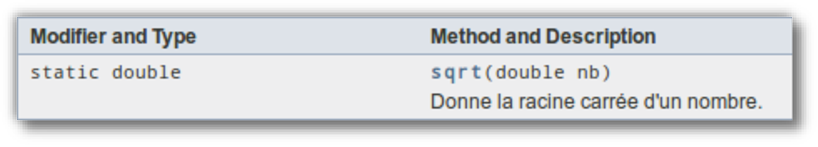
\includegraphics[scale=.6]{../img/javadoc-resume}\end{center}
\vspace{-10pt}
D�tail
\vspace{-10pt}
\begin{center}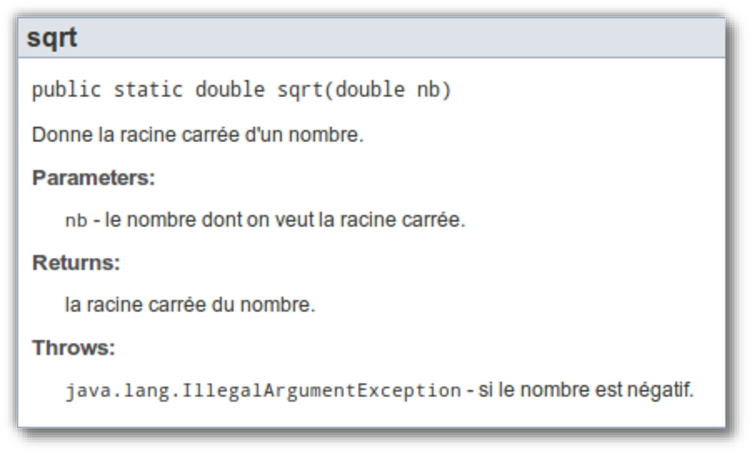
\includegraphics[scale=.6]{../img/javadoc-detail}\end{center}
\vspace{-10pt}
Remarquez tout ce qui est ajout� !
\end{frame}

\subsection{Le code HTML}

\begin{frame}[fragile]{Le code HTML}
Peut contenir des balises \sigle{HTML}
\\\medskip
\emph{Exemple} :
\begin{Java}[basicstyle=\scriptsize]
  /**
  * Indique si l'ann�e est bissextile. Pour rappel :
  * <ul>
  *   <li>Une ann�e qui n'est pas divisible par 4 n'est pas bissextile 
  *       (ex: 2009)</li>
  *   <li>Une ann�e qui est divisible par 4</li>
  *     <ul>
  *     <li>est en g�n�ral bissextile (ex: 2008)</li>
  *     <li>sauf si c'est un multiple de 100 mais pas de 400 (ex: 1900, 2100)</li>
  *     <li>les multiples de 400 sont donc bien bissextiles (ex: 2000, 2400)</li>
  *     </ul>
  *   </ul>
  * Plus formellement, <code>a</code> est bissextile si et seulement si <br/>
  * <code>a MOD 400 = 0 OU (a MOD 4 = 0 ET a MOD 100 != 0)</code>
  * @param ann�e l'ann�e dont on se demande si elle est bissextile 
  * @return vrai si l'ann�e est bissextile
  */
\end{Java}
\end{frame}

\begin{frame}{Le code HTML}
Ce qui donne
\begin{center}
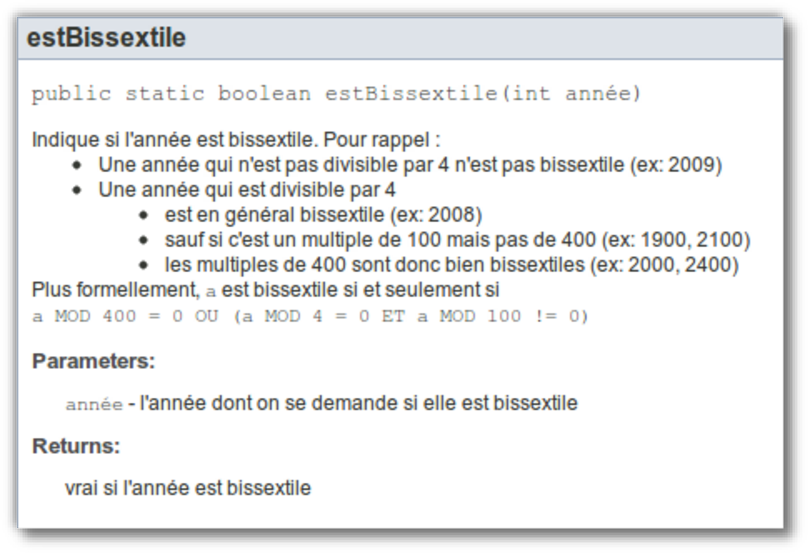
\includegraphics[scale=.7]{../img/javadoc-html}
\end{center}
\end{frame}

\subsection{Produire la documentation}

\begin{frame}[fragile]{Production de la documentation}
On utilise la commande \code|javadoc|
\begin{itemize}
\item Cr�ation de la documentation d'une classe 
\\\java|javadoc Temps.java|
\item Possibilit� de sp�cifier des sources multiples 
\\\java|javadoc *.java|
\item Cr�er la documentation dans un dossier sp�cifique 
\\\java|javadoc -d doc *.java |
\item Il y a beaucoup d'autres options \dots
\\(cf. la documentation de \sigle{javadoc})
\end{itemize}
\end{frame}

\subsection{Pour une <<bonne>> documentation}

\begin{frame}{Une bonne documentation}
Une bonne \textit{javadoc} d�crit le \emph{quoi} mais jamais le \emph{comment}
\begin{itemize}
\item $\longrightarrow$ Ne jamais parler de ce qui est priv�
\item Mauvais exemples :
  \begin{itemize}
  \item \textit{On utilise un for pour parcourir le tableau.}
  \item \textit{Pour aller plus vite, on stocke le prix hors tva dans une variable temporaire.}
  \end{itemize}
\end{itemize}
\end{frame}

\begin{frame}[fragile]{Une bonne documentation}
Ne pas �crire ce que \sigle{javadoc} �crit lui-m�me :
\begin{itemize}
\item Mauvais exemples :
  \begin{itemize}
  \item \textit{nb - un entier qui ...}
  \item \textit{La m�thode sqrt ...}
  \item \textit{Cette m�thode ne retourne rien.}
  \end{itemize}
\item Pour en savoir plus :
{\scriptsize \code|http://www.oracle.com/technetwork/java/javase/documentation/index-137868.html|}
\end{itemize}
\end{frame}

% === Cours de Java

\section{Tester le code}

\leconwithtoc

\subsection{Pr�sentation}

\begin{frame}{Pr�sentation}
Tous les programmes r�els contiennent des \emph{bugs} (erreurs, d�fauts)
\begin{itemize}
\item Parfois m�me \emph{beaucoup}
\item \emph{Inacceptable}
  \begin{itemize}
  \item \emph{Inconfort} pour l'utilisateur
  \item \emph{Perte} de temps, d'argent, de donn�es, de mat�riel
  \item Voire \emph{danger} pour la vie humaine
  \end{itemize}
\end{itemize}
\end{frame}

\begin{frame}{Pr�sentation}
Rappel des types d'erreurs
\begin{itemize}
\item � la \emph{compilation}
\item � l'\emph{ex�cution}, le programme \emph{s'arr�te}
\item � l'\emph{ex�cution}, le programme fournit une \emph{mauvaise r�ponse}
\end{itemize}
\medskip
On pourrait aussi parler d'autres d�fauts
  \begin{itemize}
  \item Trop \emph{lent}
  \item Trop gourmand en \emph{m�moire}
  \end{itemize}
\end{frame}

\begin{frame}{Pr�sentation}
\begin{center}
\emph{\og J'ai fait tourner le programme;\\il fonctionne tr�s bien ! \fg}
\end{center}
\emph{Insuffisant !} Il compile et tourne dans les cas les plus courants. Mais :
  \begin{itemize}
  \item Cas particuliers
  \item Comportement face � une d�faillance de l'environnement
  \item Comportement face � une utilisation non conforme
  \end{itemize}
\end{frame}

\begin{frame}{Pr�sentation}
Pour produire un logiciel \emph{sans bug} il faut
  \begin{itemize}
  \item Suivre une \emph{m�thodologie} �prouv�e 
    \begin{itemize}
    \item Pour produire une premi�re version avec peu de bugs \\(cf. \textit{Analyse})
    \end{itemize}
  \item \emph{Tester}, \emph{tester} et \dots \emph{ tester} encore !
    \begin{itemize}
    \item Pour d�tecter ceux qui restent
    \item Besoin d'outils pour nous aider
      \begin{itemize}
      \item Le plus facile/rapide possible
      \end{itemize}
    \end{itemize}
  \end{itemize}
\end{frame}

\subsection{Les tests}

\begin{frame}[fragile]{Les tests}
Plusieurs sortes de tests existent : unitaires, d'int�gration, fonctionnels, non-r�gression, \dots
\begin{itemize}
\item Nous ne pouvons pas tout aborder ici
\item Nous nous int�ressons aux tests \emph{unitaires} 
\end{itemize}
\medskip
\textit{Pour en savoir plus} : \code|http://fr.wikipedia.org/wiki/Test_(informatique)|
\end{frame}

\begin{frame}{Les tests}
Tests \emph{unitaires} : test de \emph{chaque m�thode} 
  \begin{itemize}
  \item Fait-elle ce qu'elle est cens�e faire ?
  \item C'est d�fini par la \textit{sp�cification} (documentation)
  \item Id�e : Si chaque m�thode est correcte \\$\longrightarrow$ le tout est correct
  \item Pas forc�ment suffisant 
\\(ex: ne teste pas la performance)
\\$\longrightarrow$ d'autres types de tests existent
\end{itemize}
\end{frame}

\subsection{Plan de tests}

\begin{frame}{Plan de tests}
Tester une m�thode ne s'improvise pas
\begin{itemize}
\item Besoin d'un \emph{plan} reprenant les tests � effectuer
  \begin{itemize}
  \item Quelles \emph{valeurs de param�tres} ?
  \item Quel est le \emph{r�sultat attendu} ?
  \end{itemize}
\item Pr�par� pendant que l'on code (ou m�me avant et �ventuellement par une autre personne)
\item Permet de s'assurer que l'on teste \emph{tous les cas}
\end{itemize}
\end{frame}

\begin{frame}{Plan de tests}
On ne peut pas tester toutes les valeurs possibles
\begin{itemize}
\item Choisir des valeurs \emph{repr�sentatives}
  \begin{itemize}
  \item Cas g�n�ral / particuliers
  \item Valeurs limites
  \end{itemize}
\item Il faut imaginer les cas qui pourraient mettre en �vidence un d�faut de la m�thode
\end{itemize}
\end{frame}

\begin{frame}{Plan de tests}
On s'inspire des erreurs les plus fr�quentes en programmation
  \begin{itemize}
  \item On commence/arr�te trop t�t/tard une boucle
  \item On initialise mal une variable
  \item Dans un test, on se trompe entre $<$ et $\leq$
  \item Dans un test, on se trompe entre $ET$ et $OU$
  \item \dots
  \end{itemize}
C'est un savoir-faire $\Longrightarrow$ Importance de l'exp�rience
\end{frame}

\begin{frame}{Plan de tests - Exemple}
\emph{Exemple} : Soit la m�thode 
\\\java|public static int max(int[] tab) {...}| 
\\qui calcule la valeur maximale d'un tableau
\begin{itemize}
\item � quoi penser en plus du cas g�n�ral ?
  \begin{itemize}
  \item Le maximum est la premi�re/derni�re valeur
  \item Le tableau ne contient qu'une seule valeur
  \item Le tableau ne contient que des nombres n�gatifs
  \end{itemize}
\end{itemize}
\end{frame}

\begin{frame}{Plan de tests - Exemple}
\begin{center}
Plan de tests de la m�thode \textit{max}
\\\bigskip
\begin{tabular}{|c|l|c|l|}
\hline
\# & tab & r�sultat & ce qui est test�\\
\hline
1 & $[1,3,0,2]$ & $3$ & cas g�n�ral\\
2 & $[1,-3,-4,-2]$ & $1$ & maximum au d�but\\
3 & $[1,3,4,11]$ & $11$ & maximum � la fin\\
4 & $[-1,-3,-4,-2]$ & $-1$ & que des n�gatifs\\
5 & $[1]$ & $1$ & tableau de taille 1\\
\hline
\end{tabular}
\end{center}
\end{frame}

\begin{frame}{Plan de tests}
\emph{Quand} tester ? Le plus \emph{souvent} possible 
\begin{itemize}
\item Erreur plus facile � identifier/corriger
\item Id�alement apr�s chaque m�thode �crite
\end{itemize}
\medskip
Que tester ? \emph{Tout}
\begin{itemize}
\item Le nouveau code peut mettre en �vidence un probl�me dans le code ancien (\emph{r�gression})
\end{itemize}
\end{frame}

\subsection{JUnit}

\begin{frame}{JUnit}
\emph{Comment} tester ?
\begin{itemize}
\item Pas � la main : intenable
\item Besoin d'un outil \emph{automatis�}
\end{itemize}
\medskip
{\small \sigle{JUnit}} : outil pour automatiser les tests unitaires
\begin{itemize}
\item Le programmeur fournit les tests,
\item \sigle{JUnit} \emph{ex�cute} tous les tests et
\item �tablit un \emph{rapport} d�taillant les probl�mes
\end{itemize}
\end{frame}

\begin{frame}{JUnit}
\begin{center}
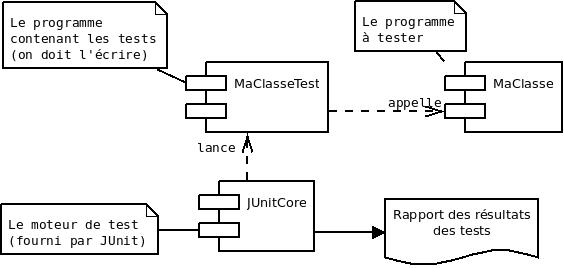
\includegraphics[scale=.5]{../img/junit} 
\end{center} 
\end{frame}

\begin{frame}{JUnit - En pratique}
La classe de test contient \emph{une m�thode} de test \emph{par cas}
  \begin{itemize}
  \item Autonome (ne re�oit rien ne retourne rien)
  \item Contient des \emph{affirmations}
    \begin{itemize}
    \item Appel de la m�thode � tester
    \item \emph{Comparaison} entre le r�sultat \emph{attendu} et le r�sultat \emph{obtenu}
    \end{itemize}
  \end{itemize}
\end{frame}

\begin{frame}[fragile]{JUnit - En pratique}
\emph{Exemple}
\begin{Java}
@Test
public void max_cas1() {
  int[] tab = {1,3,0,2};
  assertEquals( 3, max(tab) );
}
\end{Java}
{\normalsize
\begin{itemize}
\item Reconnu comme un test unitaire gr�ce � l'\emph{annotation} \java{@Test}
\item Pas de \java|static|
\item \java|assertEquals| v�rifie que les 2 valeurs sont identiques
\item Il y a aussi \java|assertTrue(val)|, \java|assertFalse(val)|, \dots
\end{itemize}
}
\end{frame}

\begin{frame}[fragile]{JUnit - En pratique}
Comment \emph{lancer} les tests ?
\begin{Java}
java org.junit.runner.JUnitCore MaClasseTest
\end{Java} %$
\medskip
R�sultat ?
\begin{itemize}
\item Nb de (m�thodes de) tests effectu�s / r�ussis
\item D�tail sur les tests rat�s
  \begin{itemize}
  \item Nom du test
  \item R�sultat obtenu compar� au r�sultat attendu
  \end{itemize}
\end{itemize}
\end{frame}

\begin{frame}[fragile]{JUnit - Exemple}
\emph{Exemple} : soit le code suivant � tester
\begin{Java}
package be.heb.esi.java1;

public class Outil {
  public static int max(int[] tab) {
    int max = 0;
    for(int i=0; i<tab.length; i++) {
      if (tab[i]>max) {
        max = tab[i];
      }
    }
    return max;
  }
}
\end{Java}
\end{frame}

\begin{frame}[fragile]{JUnit - Exemple}
La classe de test donnerait
\begin{Java}
package be.heb.esi.java1;
import org.junit.Test;  // Pour que @Test soit connu
import static org.junit.Assert.*; // Pour assertEquals

public class OutilTest {
  @Test public void max_cas1() {
    int [] tab = {1,3,0,2};
    assertEquals( 3, Outil.max(tab) );
  }

  @Test public void max_cas4() {
    int [] tab = {-1,-3,-4,-2};
    assertEquals( -1, Outil.max(tab) );
  }

  // + plus les cas 2, 3 et 5
}
\end{Java}
\end{frame}

\begin{frame}[fragile]{JUnit - Exemple}
On peut compiler la classe de test et la donner au moteur de test
\begin{Java}
javac OutilTest.java
java org.junit.runner.JUnitCore be.heb.esi.java1.OutilTest
JUnit version 4.5
..E
Time: 0,02
There was 1 failure:
1) max_cas4(OutilTest)
java.lang.AssertionError: expected:<-1> but was:<0>
[...]
FAILURES!!!
Tests run: 2,  Failures: 1
\end{Java} %$
Une id�e du probl�me ?
\end{frame}

\begin{frame}[fragile]{JUnit - Tester les exceptions}
Imaginons une m�thode \java|sqrt| pour calculer la racine carr�e d'un entier
\begin{itemize}
\item Hypoth�se : elle doit lancer une exception en cas de param�tre n�gatif
\item Le code pourrait ressembler � ceci
\begin{Java}
public static int sqrt(int val) {
    if (val<0) {
        throw new IllegalArgumentException(
            "Pas de racine car�e pour un entier n�gatif");
    }
    // suite : calcul de la racine carr�e
}
\end{Java}
\end{itemize}
\end{frame}

\begin{frame}[fragile]{JUnit - Tester les exceptions}
� priori c'est correctement �crit mais il faut le tester !
\begin{Java}
@Test(expected=IllegalArgumentException.class)
public void sqrt_cas_n�gatif() {
  sqrt(-1);
}
\end{Java}
\begin{itemize}
\item Le test est r�ussi si la m�thode lance l'\emph{exception} indiqu�e
\end{itemize}
\end{frame}

\subsection{Conclusion}

\begin{frame}{Conclusion}
\emph{\og Il faut vraiment tout tester ? \fg}
\begin{itemize}
\item Compromis entre le temps que l'on consacre aux tests et la probabilit� de trouver une erreur
\item Trop simple $\longrightarrow$ perte de temps
\item Attention ! On commet vite une erreur m�me dans du code simple
\item De plus, les tests unitaires aident � la <<refactorisation>> (cf. la le�on sur la lisibilit�)
\end{itemize}
\end{frame}

\begin{frame}[fragile]{Conclusion}
\begin{center}
\textit{\og \emph{Any program feature without \\an automated test simply doesn't exist.}\fg}
\\Kent Beck in \textit{Extreme Programming Explained}.
\end{center}
Pour aller plus loin :
  \begin{itemize}
  \item Le site de \sigle{JUnit} : \code|http://www.junit.org|
  \item La Javadoc : \code|http://junit.sourceforge.net/javadoc|
  \item T�l�charger \sigle{JUnit} : \code|http://sourceforge.net/projects/junit/files/junit|
  \end{itemize}
\end{frame}




% === Cours de Java
% === Chapitre : Les donn�es

\section{Variables locales}

\leconwithtoc

\subsection{Pr�sentation}

\begin{frame}{Pr�sentation}
D�signation g�n�rique d'un \emph{emplacement} de la \emph{m�moire vive}
\begin{itemize}
\item \emph{Poss�de un type}
\item Ne peut contenir que des valeurs de ce type
\item Allocation diff�rente si type \\\emph{primitif} ou \emph{r�f�rence}
\end{itemize}
\end{frame}

\subsection{Allocation m�moire}

\begin{frame}{Allocation m�moire}
Pour un type \emph{primitif}
\begin{itemize}
\item Indique la zone m�moire (sur la pile/{\it stack}) o� se trouve la \emph{valeur}
\end{itemize}
\vspace{-1ex}
\begin{center}
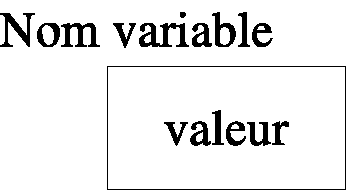
\includegraphics[scale=.4]{../img/java-data-primitive} 
\end{center}
\pause
Pour un type \emph{r�f�rence} (ex: \java|String|, tableau)
\begin{itemize}
\item La zone m�moire contient l'\emph{adresse} de la zone m�moire (sur le tas/{\it heap}) contenant la valeur (indirection)
\end{itemize} 
\begin{center}
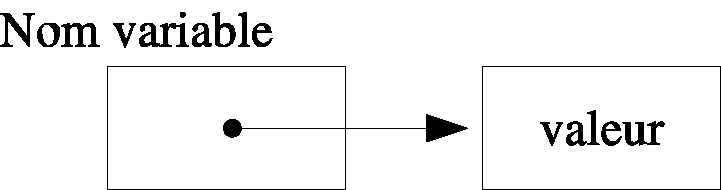
\includegraphics[scale=.4]{../img/java-data-reference} 
\end{center}
\end{frame}

\subsection{D�claration}

\begin{frame}[fragile]{D�claration}
D�claration locale � un \emph{bloc}
\begin{grammaire}
\nterm{Block} :
    \term{\{} \nterm{BlockStatements}\opt \term{\}}

\nterm{BlockStatements} :
    \nterm{BlockStatement}
    \nterm{BlockStatements}  \nterm{BlockStatement}

\nterm{BlockStatement} :
    \nterm{LocalVariableDeclarationStatement}
    \nterm{Statement}
\end{grammaire}
Peut-on m�langer d�clarations et instructions ?
\end{frame}

\begin{frame}[fragile]{D�claration}
\par {\small (r�gles l�g�rement simplifi�es)}
\begin{grammaire}
\nterm{LocalVariableDeclarationStatement} :
    \term{final}\opt \nterm{Type} \nterm{VariableDeclarators} \term{;}

\nterm{VariableDeclarators} :
    \nterm{VariableDeclarator}
    \nterm{VariableDeclarators} \term{,} \nterm{VariableDeclarator}

\nterm{VariableDeclarator} :
    \nterm{Identifier}
    \nterm{Identifier} \term{=} \nterm{Expression}
\end{grammaire}
\begin{itemize}
\item \emph{Exemples} :
\begin{itemize}
\item \java|int i;|
\item \java|String nom, pr�nom;|
\item \java|boolean ok=true, fini;|
\item \java|char lettre, chiffre='1';| 
\end{itemize}
\end{itemize}
\end{frame}

\subsection{Conventions sur les noms}

\begin{frame}{Nom d'une variable}
Quel nom peut-on choisir ? Diff�rence entre
  \begin{itemize}
  \item Ce qui est permis par \sigle{Java}
  \item Les conventions suppl�mentaires
  \end{itemize}
\bigskip
R�gles \emph{impos�es} par la grammaire
\begin{itemize}
\item Longueur illimit�e
\item Compos� de \textit{lettres}, de \textit{chiffres}, \java|$| et \java|_| %$
\\(internationalisation)
\item Ne commence pas par un chiffre
\item $\neq$ \nterm{keyword} ou \nterm{litteral}
\item Ex valides : \java|nom|, \java|Nom|, \java|Nom23|, \java|Unpeu2touT|%$
\item Ex invalides : \java|2main|, \java|le total|, \java|for|, \java|true|, \java|12|
\end{itemize}
\end{frame}

\begin{frame}[fragile]{Nom d'une variable}
Conventions \emph{suppl�mentaires}
\begin{itemize}
\item Utilis�es dans le monde entier
\begin{itemize}
\item Eviter \java|$| et \java|_| %$
\item Commence par une minuscule
\item Plusieurs mots accoll�s $\Rightarrow$ les suivants commencent par une majuscule ({\it mixedcase})
\item Noms explicites (sauf abr�viations courantes)
\item Articles omis
\end{itemize} 
\item Autres recommandations de \sout{\sigle{Sun}} \sigle{Oracle}
\begin{itemize}
\item D�clarer en d�but de bloc
\item Une d�claration par ligne
\end{itemize} 
\end{itemize}
\end{frame}

\subsection{Valeur initiale}

\begin{frame}[fragile]{Valeur initiale}
On peut indiquer une \emph{valeur initiale} 
\\(par \emph{d�faut}, \emph{aucune} valeur n'est assign�e)
\begin{itemize}
\item N'importe quelle expression calculable � cet endroit l� (� l'ex�cution)
\item Exemple
\begin{Java}
int poidsKilo = 20; // Un poids en kilos
int poidsGramme = 1000*poidsKilo; // L'�quivalent en grammes
\end{Java}  
\item Exemple
\begin{Java}
int poidsKilo; // Un poids en kilos
int poidsGramme = 1000*poidsKilo; // erreur � la COMPILATION
\end{Java}  
\end{itemize} 
\end{frame}

\subsection{Le concept de <<port�e>>}

\begin{frame}{Scope (port�e) d'une variable locale}
D�finition : Le \emph{\textit{scope}} (\emph{port�e}) d'une variable indique la portion du programme o� elle \textit{existe}
\par\medskip
Le \textit{scope} d'une variable locale est
\begin{itemize}
\item le \textit{block} de sa d�claration (entre \java|\{\}|)
\item d�s sa propre initialisation
\end{itemize} 
\end{frame}

\begin{frame}[fragile]{Scope (port�e) d'une variable locale}
\emph{Exemples} : bon ou pas ?
\begin{Java}
{
   int x = y; 
   int y = 1;
}
\end{Java}
\begin{Java}
{
   int x;
   int y = x; 
}
\end{Java}
\begin{Java}
{
  int x = 1, y = x; 
}
\end{Java}
\end{frame}

\subsection{Constantes}

\begin{frame}[fragile]{Constante}
Clause \java|final| $\Rightarrow$ constante
\begin{itemize}
\item Valeur donn�e
\begin{itemize}
\item Soit � la d�claration 
\item Soit par assignation ult�rieure
\end{itemize} 
\begin{Java}
  final int X = 1;
  final int Y;
  Y = 2*X;
  X = 2; // Erreur : poss�de d�j� une valeur
  Y = 3; // Idem
\end{Java}
\item Pourquoi une constante au lieu d'un litt�ral ?
\end{itemize} 
\end{frame}

\begin{frame}[fragile]{Constante}
Convention de nom diff�rente
\begin{itemize}
\item Tout mettre en \emph{majuscules}
\item Utiliser \java|_|  pour s�parer les mots
\end{itemize} 
\emph{Exemples}
\begin{Java}
  final double PI = 3.1415;
  final int TAUX_TVA = 21;
\end{Java}
\end{frame}


% === Cours de Java
% === Chapitre : Les expressions

\section{Les expressions}

\leconwithtoc

\begin{frame}[fragile]{D�finitions}
\emph{Expression}: calcul faisant intervenir une ou plusieurs valeur(s) pour une op�ration d�termin�e
\\\bigskip
\emph{Exemple} : \java|1+2|
  \begin{itemize}
  \item \java|1| et \java|2| sont les op�randes
  \item \java|+| est l'op�rateur
  \item l'expression est de type \java|int|
  \item la valeur de l'expression est $3$
  \end{itemize}
\end{frame}

\subsection{Les expressions enti�res}

\begin{frame}[fragile]{Les expressions enti�res}
\emph{Op�rateurs}
  \begin{itemize}
  \item unaires : \java|+| et \java|-|
  \item binaires : \java|+|, \java|-|,\java|*|, \\\java|/| (division enti�re) et \java|%| (modulo) %
  \end{itemize}
\medskip
\emph{Op�randes} pouvant intervenir
\begin{itemize}
\item un \emph{litt�ral} : \java|1 + 2| vaut $3$
\item une \emph{variable}
\begin{itemize}
\item si $i$ vaut 3, \java|i + 2| vaut $5$ 
\item si $i$ vaut 3, \java|i + i| vaut  $6$ 
\end{itemize} 
\item une \emph{expression}
\begin{itemize}
\item si $i$ vaut 3, \java|(i + i) + 2| vaut $8$ 
\end{itemize} 
\end{itemize}
\end{frame}

\begin{frame}[fragile]{Les expressions enti�res}
Uniquement avec des op�randes d'un \emph{m�me} type entier
\begin{itemize}
\item Type de l'expression = celui de ses op�randes
\item Exemples :
  \begin{itemize}
  \item \java|1 + 2| vaut $3$ de type \java|int| 
  \item \java|1L + 2L| vaut $3$ de type \java|long| 
  \item \java|3 / 2| vaut $1$ de type \java|int| 
  \end{itemize}
\end{itemize}
\end{frame}

\begin{frame}[fragile]{Priorit� et associativit�}
Probl�me avec l'expression : \java|i + i * 2|
  \begin{itemize}
  \item Le compilateur va-t-il comprendre
    \begin{itemize}
    \item \java|(i+i) *2| ?
    \item \java|i+ (i*2)| ?
    \end{itemize} 
  \end{itemize} 
\bigskip
La strat�gie d'�valuation se base sur
  \begin{itemize}
  \item la \emph{priorit�} d'un op�rateur
  \item l'\emph{associativit�} des op�rateurs de m�me priorit�
  \end{itemize} 
\begin{center}
\begin{tabular}{r|c|c}
 priorit� & op�rateur & associativit� \\ \hline
grande & \java|-|, \java|+| unaires & $\Longleftarrow$ \\
 & \java|*|, \java|/|, \java|%| & $\Longrightarrow$ \\
faible & \java|-|, \java|+| binaires & $\Longrightarrow$ \\
\end{tabular}
\end{center}
\end{frame}

\begin{frame}[fragile]{Tableau des priorit�s et associativit�s}
\emph{Exercices} : comment comprendre
  \begin{itemize}
  \item \java|3 + 3 * 2 + 1| ?
  \item \java|3 + 3 * 2 / - 4 + 5 % 8| ?
  \end{itemize}  
\bigskip
\emph{Parenth�ses} pour forcer la strat�gie 
  \begin{itemize}
  \item Exemple : \java|(3 + 3) * (2 + 1)| $\rightarrow$ \java|6 * 3|  $\rightarrow$ \java|18|
  \end{itemize}
\bigskip
Moralit�: mieux vaut parenth�ser compl�tement
  \begin{itemize}
  \item \emph{ordre explicite} de l'�valuation 
  \item \emph{clart�} pour les autres utilisateurs
  \end{itemize} 
\end{frame}

\begin{frame}{Erreurs de calcul}
La \emph{division par z�ro} 
\begin{itemize}
\item Lance une \textit{exception} (\textit{ArithmeticException})
\item Pour l'instant, \emph{arr�te le programme} avec un message explicite
\end{itemize} 
\bigskip
Le \emph{d�passement de capacit�} 
\begin{itemize}
\item N'est \emph{pas d�tect�} par la machine virtuelle
\item Le r�sultat est tout simplement faux
\end{itemize} 
\end{frame}

\subsection{Les expressions flottantes}

\begin{frame}[fragile]{Les expressions flottantes}
Uniquement avec les op�randes d'un m�me type \emph{flottant}
\begin{itemize}
\item Type de l'expression = type des op�randes
\item Op�rateurs unaires : \java|+| et \java|-|
\item Op�rateurs binaires : \java|+|, \java|-|,\java|*|, \java|/|
\item Le reste est identique aux entiers
\end{itemize}
\smallskip
\emph{Exemples} : Donner la valeur et le type de 
\begin{itemize}
\item \java|1.0 + 2.3| 
\item \java|1.0d - 2.3d|
\item \java|7.0f / 3.5f|  
\item \java|1. / 3.|
\end{itemize} 
\end{frame}

\subsection{Les expressions caract�res}

\begin{frame}[fragile]{Les expressions caract�res}
\java|char| est un type num�rique entier
\begin{itemize}
\item \emph{Aucun op�rateur} sp�cifique 
\item On pourrait effectuer des calculs mais non recommand�
  \\\emph{Exemple} : \java|'a' + 'b'|
\end{itemize}
\end{frame}

\subsection{Les chaines de caract�res}

\begin{frame}[fragile]{Les chaines de caract�res}
Un seul op�rateur (binaire) disponible :
  \begin{itemize}
  \item \java|+| : concat�nation de deux chaines
  \item \emph{Ex} : \java|"Ja"| + \java|"va"| vaut \java|"Java"|
  \end{itemize}
\bigskip
Conversion si un des 2 op�randes n'est pas une chaine.
  \begin{itemize}
  \item \emph{Ex} : \java|""+3.5| vaut \java|"3.5"|
  \item \emph{Ex} : \java|"1"+2+3| vaut \java|"123"|
  \item \emph{Ex} : \java|1+"2"+3| vaut \java|"123"|
  \item \emph{Ex} : \java|1+2+"3"| vaut \java|"33"| !
  \end{itemize}
\end{frame}

\subsection{Les expressions bool�ennes}

\begin{frame}[fragile]{Les expressions bool�ennes}
Op�rateurs :
\begin{itemize}
\item unaire : \java|!| (non)
\item binaires : \java|&&| (et) et \java{||} (ou)
\end{itemize}
\begin{center}
\begin{tabular}{r|c|c}
 priorit� & op�rateur & associativit� \\ \hline
grande & \java|-|, \java|+| unaires, \java|!| & $\Longleftarrow$ \\
 & \java|*|, \java|/|, \java|%| & $\Longrightarrow$ \\
 & \java|-|, \java|+| binaires & $\Longrightarrow$ \\
 & \java|&&| & $\Longrightarrow$ \\
faible & {\color{blue!70!black} \verb,||,} & $\Longrightarrow$ \\
\end{tabular}
\end{center}
\end{frame}

\begin{frame}[fragile]{Les expressions bool�ennes}
\java|&&| : table de v�rit� \\
\medskip
\begin{center}
\begin{tabular}{c|c|c|} 
(ET) & \java|true| & \java|false| \\ \hline
\java|true| & \java|true| & \java|false| \\ \hline
\java|false| & \java|false| & \java|false| \\ \hline
\end{tabular} 
\end{center}
\medskip
Particularit� : si l'op�rande de gauche est \emph{faux}, l'op�rande droit \emph{ne sera pas �valu�} et le r�sultat sera \java|false| 
\end{frame}

\begin{frame}[fragile]{Les expressions bool�ennes}
\java{||} : table de v�rit� \\
\begin{center}
\begin{tabular}{c|c|c|} 
(OU) & \java|true| & \java|false| \\ \hline
\java|true| & \java|true| & \java|true| \\ \hline
\java|false| & \java|true| & \java|false| \\ \hline
\end{tabular} 
\end{center}
\medskip
Particularit� : si l'op�rande de gauche est \emph{vrai}, l'op�rande droit \emph{ne sera pas �valu�} et le r�sultat sera \java|true| 
\end{frame}

\begin{frame}[fragile]{Exemples}
Comment �valuer ?
\begin{itemize}
\item \java{true && false || true} 
\item \java{false || false && ! true} 
\item \java{true || false && true} 
\item \java{false && (true || false)} 
\item \java{!(true || false) && true} 
\end{itemize} 
\end{frame}

\begin{frame}[fragile]{R�sum�}
Voici les r�gles qui r�sument tout ceci
\begin{grammaire}
\nterm{Expression} :
    \nterm{ConditionalOrExpression}

\nterm{ConditionalOrExpression} :
    \nterm{ConditionalAndExpression}
    \nterm{ConditionalOrExpression}  \term{||} \nterm{ConditionalAndExpression}

\nterm{ConditionalAndExpression} :
    \nterm{AdditiveExpression}
    \nterm{ConditionalAndExpression} \term{&&} \nterm{AdditiveExpression}

\nterm{AdditiveExpression} :
    \nterm{MultiplicativeExpression}
    \nterm{AdditiveExpression} \term{+} \nterm{MultiplicativeExpression}
    \nterm{AdditiveExpression} \term{-} \nterm{MultiplicativeExpression}
\end{grammaire} 
\end{frame}

\begin{frame}[fragile]{R�sum�}
\begin{grammaire}
\nterm{MultiplicativeExpression} :
    \nterm{UnaryExpression}
    \nterm{MultiplicativeExpression} \term{*} \nterm{UnaryExpression}
    \nterm{MultiplicativeExpression} \term{/} \nterm{UnaryExpression}
    \nterm{MultiplicativeExpression} \term{%} \nterm{UnaryExpression}

\nterm{UnaryExpression} :
    \term{+} \nterm{UnaryExpression}
    \term{-} \nterm{UnaryExpression}
    \term{!} \nterm{UnaryExpression}
    \nterm{Literal}
    \term{(} \nterm{Expression} \term{)}
    \nterm{Identifier}
\end{grammaire} 
\begin{itemize}
\item On y voit la priorit� et l'associativit� des op�rateurs
\item Pas suffisant pour int�grer toutes les contraintes additionnelles (par exemple ?)
\end{itemize} 
\end{frame}

\subsection{Les expressions relationnelles}

\begin{frame}[fragile]{Les expressions relationnelles}
Op�rateurs de comparaison et d'�galit�
\begin{itemize}
\item Op�randes doivent �tre de \emph{m�me type}
\item Le \emph{r�sultat} est du type \emph{boolean}
\end{itemize} 
\bigskip
Op�rateurs de \emph{comparaison} : {\small \java|<|,\java|>|,\java|<=| et \java|>=|}
  \begin{itemize}
  \item Uniquement pour des \emph{types num�riques} 
  \item Exemple : \java|true < false| n'est pas accept�
  \item Exemple : \java|"Absolu" < "Relatif"| non plus 
  \end{itemize} 
\end{frame}

\begin{frame}[fragile]{L'�galit� de valeurs}
Op�rateurs d'\emph{�galit�} : \java|==| et \java|!=|
  \begin{itemize}
  \item S'appliquent � \emph{tous les types}
  \item Exemple : \java|true == false| est \java|false|
  \item Sens diff�rent si type primitif ou r�f�rence
  \end{itemize}
\bigskip
Type primitif : les \emph{valeurs} sont compar�es
\begin{center}
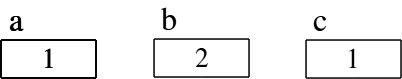
\includegraphics[scale=.5]{../img/java-logi-egal1} 
\end{center}
On a : \java|a==c| mais \java|a!=b| et \java|b!=c|
\end{frame}

\begin{frame}[fragile]{�galit� de valeurs}
Type r�f�rence : les \emph{r�f�rences} sont compar�es
\begin{center}
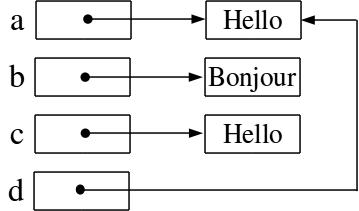
\includegraphics[scale=.5]{../img/java-logi-egal2} 
\end{center}
On a : \java|a!=b|, \java|a!=c| mais \java|a==d|
\end{frame}

\begin{frame}[fragile]{Particularit� du type String}
\begin{Java}
{
  String s1 = "Hello";
  String s2 = "Hello";
  String s3 = "Hel";
  s3 = s3 + "lo";
  System.out.println(s1==s2); // Vrai
  System.out.println(s1==s3); // Faux
}
\end{Java}
\begin{itemize}
\item R�utilisation de l'espace mais pour les litt�raux uniquement
\item Pas si r�sultat d'un \emph{calcul} ou \emph{lecture} au clavier
\end{itemize}
\end{frame}

\begin{frame}[fragile]{Egalit� de valeur}
Pour les types r�f�rences, on peut aussi utiliser la m�thode \java|equals| 
\begin{itemize}
\item Ne teste pas que les r�f�rences sont identiques
\item Mais bien que les \emph{valeurs} r�f�renc�es sont �gales
\end{itemize}
\begin{Java}
{
  String s1 = "Hello";
  String s2 = "Hello";
  String s3 = "Hel";
  s3 = s3 + "lo";
  System.out.println(s1.equals(s2)); // Vrai
  System.out.println(s1.equals(s3)); // Vrai
}
\end{Java}
\end{frame}

\subsection{Les expressions conditionnelles}

\begin{frame}[fragile]{L'expression conditionnelle}
�quivalent du \emph{si-sinon} sous forme d'expression
\begin{Java}
  condition ? si valeur vrai : si valeur faux 
\end{Java} 
\begin{itemize}
\item Parfois plus lisible mais ne pas abuser
\item C'est une expression, elle a une valeur
\end{itemize}
\medskip
\emph{Exemples}
\begin{itemize}
\item Quel type a l'expression : \java{heure < 12 ? "bonjour" : "bonsoir"}
\item Que vaudra abs ? 
\begin{Java}
int n = -4; 
int abs = n > 0 ? n : -n;
\end{Java}
\end{itemize}
\end{frame}

\begin{frame}[fragile]{Tableau des priorit�s et associativit�s}
(op�rateurs d�j� vus)
\begin{small}
\begin{center}
\begin{tabular}{r|c|c}
 priorit� & op�rateur & associativit� \\ \hline
grande & \java|-|, \java|+| unaires, \java|!| & $\Longleftarrow$ \\
 & \java|*|, \java|/|, \java|%| & $\Longrightarrow$ \\
 & \java|-|, \java|+| binaires & $\Longrightarrow$ \\
 & \java|<|, \java|>|, \java|<=|, \java|>=| & $\Longrightarrow$ \\
 & \java|==|, \java|!=| & $\Longrightarrow$ \\
 & \java|&&| & $\Longrightarrow$ \\
 & {\color{blue!70!black} \verb,||,} & $\Longrightarrow$ \\
faible & {\color{blue!70!black} \verb,?:,} & $\Longleftarrow$ \\
\end{tabular}
\end{center}
\end{small}
\end{frame}

\subsection{Un mot sur les conversions}

\begin{frame}{Un mot sur les conversions}
Peut-on m�langer les types ?
\begin{itemize}
\item Normalement pas
\item Accept� si pas de perte d'information
\item \emph{Conversion} effectu�e \emph{automatiquement} par le compilateur
\item Une le�on enti�re sera consacr�e � ce sujet
\end{itemize}
\end{frame}

\begin{frame}[fragile]{Un mot sur les conversions}
Voyons les situations les plus fr�quentes
\begin{itemize}
\item Calcul m�langeant les entiers et les r�els
  \begin{itemize}
  \item Les entiers sont convertis en r�els
  \item \emph{Ex} : \java|3.2/2| vaut $1.6$ de type \java|double|
  \end{itemize}
\item Assigner un entier � un r�el
  \begin{itemize}
  \item L'entier est converti en r�el
  \item \emph{Ex} : \java|double d = 1; // d vaut 1.0|
  \end{itemize}
\item Assigner un r�el � un entier
  \begin{itemize}
  \item Refus� \dots\ sauf si demand� explicitement (\emph{casting})
  \item \emph{Ex} : \java|int i = 1.2; // refus�|
  \item \emph{Ex} : \java|int j = (int) 1.6; // j vaut 1|
  \end{itemize}
\end{itemize}
\end{frame}
  
% === Cours de Java
% === Chapitre : Les instructions expressions

\section{Les assignations}

\begin{frame}[c]
\begin{block}{\center Le\c con \thesection}
  {
  \begin{center}
  Les assignations\\(et autres \og expressions - instructions\fg)
  \bigskip
  \tableofcontents[sectionstyle=hide,subsectionstyle=show/show/hide]
  \bigskip
  \end{center}
  }
\end{block}
\end{frame}

\subsection{Les assignations}

\begin{frame}[fragile]{L'assignation}
(version l�g�rement simplifi�e)
\begin{itemize}
\begin{grammaire}
  \nterm{Assignment} :
      \nterm{LeftHandSide} \term{=} \nterm{Expression}

  \nterm{LeftHandSide} :
      \nterm{Identifier}
      \nterm{ArrayAccess}
\end{grammaire}
\item \emph{Exemples}
\begin{Java}
brol = 1
brol[i]=j
\end{Java}
\item Tiens ! Pas de \java|;| � la fin ?
\end{itemize}
\end{frame}

\begin{frame}[fragile]{Les expressions instructions}
En fait, l'assignation est une \emph{expression}
  \begin{itemize}
  \item qui peut devenir une \emph{instruction} ({\it statement})
  \item par ajout d'un \java{;}
  \item la valeur est perdue
  \end{itemize}
Une expression qui peut devenir une instruction s'appelle une \emph{\it statement expression} 
\begin{grammaire}
  \nterm{Statement} :                              \nterm{ExpressionStatement} :
      \nterm{ExpressionStatement}                      \nterm{StatementExpression} \term{;}
      (...)

  \nterm{StatementExpression} :
      \nterm{Assignment}
      (...)
\end{grammaire}
\end{frame}

\begin{frame}{L'assignation - expression}
Une \emph{assignation} est d'abord une \emph{expression}
\begin{itemize}
\item Son type : le type de la variable
\item Sa valeur : la valeur du \textit{left hand side}
\item Peut donc intervenir comme �l�ment d'une autre expression
\item Priorit� faible et associative de \textit{droite � gauche}
\end{itemize}
\end{frame}

\begin{frame}[fragile]{L'assignation - expression}
Ceci explique pourquoi on peut �crire
\begin{Java}
  i = j = k = l = 0;
  i = (j = i+j) + 1;
  f(i=1,j=0);
  while( (i=i-1) != 0 ) {...}
  while( ok=true ) {...}  // boucle infinie !
\end{Java}
Mais pas
\begin{Java}
  i = j = k = l = 0	  // erreur compilation
  while( ok=true; ) {...} // idem
\end{Java}
\end{frame}

\begin{frame}[fragile]{Autres Assignations}
Il existe d'autres \emph{op�rateurs d'assignation}
  \begin{grammaire}
  \nterm{Assignment} :
          \nterm{LeftHandSide}   \nterm{AssignmentOperator}   \nterm{Expression}

  \nterm{AssignmentOperator} : one of \term{=} \term{*=} \term{/=} \term{%=} \term{+=} \term{-=}
  \end{grammaire}
\begin{itemize}
\item \java|var += expr| �quivaut � \java|var = var + expr|
\item \emph{Ex} : \java|i+=1| �quivaut � \java|i = i + 1|
\item Que penser de ?
\begin{Java}
 i = 2; 
 i = i = (i*=2) + 1;
 (i+1) -= 2;
\end{Java}
\end{itemize}
\end{frame}

\begin{frame}[fragile]{Les expressions instructions}
Existe-t-il d'autres \textit{expressions instructions} ? 
\begin{grammaire}
  \nterm{StatementExpression} :
     \nterm{Assignment}
     \nterm{PreIncrementExpression}
     \nterm{PreDecrementExpression}
     \nterm{PostIncrementExpression}
     \nterm{PostDecrementExpression}
     \nterm{MethodInvocation}

     \nterm{ClassInstanceCreationExpression} (cf. OO)
\end{grammaire}
\end{frame}

\subsection{Post/pr� incr�mentation/d�cr�mentation}

\begin{frame}[fragile]{Post/pr� incr�mentation/d�cr�mentation}
\java|++| permet d'incr�menter une variable
  \begin{itemize}
  \item Peut se placer avant ou apr�s la variable
  \item \java|i++;| $\equiv$ \java|++i;| $\equiv$\java|i+=1;| $\equiv$ \java|i=i+1;|
  \end{itemize}
\bigskip
Il existe tout de m�me une diff�rence
  \begin{itemize}
  \item \java|++i| : \java|i| est incr�ment� \emph{avant} d'�tre utilis�
  \item \java|i++| : \java|i| est incr�ment� \emph{apr�s} avoir �t� utilis�
  \item \emph{Exemples}
  \begin{Java}
    int i = 5;
    j = i++;
    j = ++i;
    System.out.println(i++);
  \end{Java}
  \end{itemize}
\end{frame}

\begin{frame}[fragile]{Post/pr� incr�mentation/d�cr�mentation}
Pr�cisons.
\begin{itemize}
\item Avec \java|i++| :
  \begin{enumerate}
  \item \java|i| donne sa valeur � l'expression \java|i++|
  \item \java|i| est incr�ment�
  \end{enumerate}
\item Avec \java|++i| :
  \begin{enumerate}
  \item \java|i| est incr�ment�
  \item \java|i| donne sa valeur � l'expression \java|++i|
  \end{enumerate}
\end{itemize}
\emph{Exemples}
  \begin{Java}
    int i = 5;
    i = i++;
    i = ++i;
    i = i++ + ++i;
    i = ++i + i++;
    i = (i++)++;    
    i = 2++;        
  \end{Java}
\end{frame}

\begin{frame}[fragile]{Post/pr� incr�mentation/d�cr�mentation}
\emph{Exercice} : Qu'affichent les bouts de code suivants
\begin{Java}
for(int i=0; i<5; i++) {
    System.out.println(i);
}
\end{Java}
\begin{Java}
for(int i=0; i<5; ++i) {
    System.out.println(i);
}
\end{Java}
\begin{Java}
for(int i=0; i<5; i++) {
    System.out.println(i++);
}
\end{Java}
\begin{Java}
for(int i=0; ++i<5; ) {
    System.out.println(i);
}
\end{Java}
\end{frame}

\begin{frame}[fragile]{Post/pr� incr�mentation/d�cr�mentation}
\java|--| fonctionne comme \java|++| mais d�cr�mente
  \begin{itemize}
  \item Exemples
  \begin{Java}
    int i = 5;
    i = i--;
    i = i-- - ++i;
  \end{Java}
  \end{itemize}
\bigskip
Comment comprendre ceci ?
\begin{itemize}
  \item[]
  \begin{Java}
    i = i++  +  i;    
    i = i-  --  i;    
    i = i+++1;      
    i = i--  - -- i; 
    i = i+++++i;    
  \end{Java}
  \item Aide : penser au fonctionnement du compilateur 
  \end{itemize}
\end{frame}

\begin{frame}[fragile]{Tableau des priorit�s et associativit�s}
\begin{center}
\begin{footnotesize}
\begin{tabular}{c|r|l|c}
priorit� & & & associativit� \\ \hline
forte & postfixes unaires & \java|(params)|, \java|.|, \java|expr++|, \java|expr--| & $\Longrightarrow$ \\ 
       & pr�fixes unaires & \java|++expr|, \java|--expr|, \java|-|, \java|+|, \java|!|, \java|new| & $\Longleftarrow$ \\
       & multiplicatif & \java|*|, \java|/|, \java|%| & $\Longrightarrow$  \\
       & additif & \java|-|, \java|+|  & $\Longrightarrow$ \\
       & relationnels & \java|<|, \java|>|, \java|<=|, \java|>=| & $\Longrightarrow$  \\
       & �galit� & \java|==|, \java|!=| & $\Longrightarrow$  \\
       & et & \java|&&| & $\Longrightarrow$  \\
       & ou & {\color{blue!70!black} \verb,||,} & $\Longrightarrow$  \\
       & condition & \java|:?| & $\Longleftarrow$  \\
faible  & assignations & \java|=|, \java|+=|, \java|-=|, \java|*=|, \java|/=|, \java|%=| & $\Longleftarrow$   \\
\end{tabular}
\end{footnotesize}
\end{center}
\end{frame}

\begin{frame}[fragile]{Ordre d'�valuation}
Comment comprendre ceci ?
\begin{itemize}
\begin{Java}
  i = 2;
  i = (i=3) * i;
  i = i * ++i;
\end{Java}
\item Probl�me dans beaucoup de langages
\item En \sigle{Java}, \emph{�valuation garantie de gauche � droite} 
\end{itemize}
\bigskip
Aussi pour les param�tres d'un appel de m�thode
\begin{Java}
  i = 2;
  f(i++,--i); // �quivaut � f(2,2)
  f(--i,i++); // �quivaut � f(1,1)
\end{Java}
\end{frame}

\subsection{Appel de m�thode}

\begin{frame}[fragile]{Appel de m�thode}
L'\emph{appel de m�thode} est un autre cas d'expression-instruction
\begin{itemize}
\item Explique pourquoi ceci est valable
\begin{Java}
a = f(1);  
f(1);      
Math.sqrt(4);
\end{Java}
\item La valeur de retour est \emph{perdue} !
\end{itemize}
\end{frame}

\subsection{Recommandation}

\begin{frame}{Recommandation}
\emph{Comment utiliser} les assignations (en tous genres) ?
\\\medskip
Afin d'assurer une bonne lisibilit� du code :
\begin{itemize}
\item \emph{Jamais} comme une \emph{expression}
\item Mais \emph{toujours} comme une \emph{instruction}
\end{itemize}
\end{frame}



 
% === Cours de Java
% === Chapitre : Les expressions

\section{Instructions}

\leconwithtoc

\begin{frame}[fragile]{Les instructions}
\begin{grammaire}
 \nterm{Statement} :
     \nterm{Block}					
     \nterm{EmptyStatement}			
     \nterm{LabeledStatement}
     \nterm{BreakStatement}
     \nterm{ContinueStatement}
     \nterm{ExpressionStatement}
     \nterm{IfThenStatement}
     \nterm{IfThenElseStatement}
     \nterm{SwitchStatement}
     \nterm{WhileStatement}
     \nterm{DoStatement}
     \nterm{ForStatement}
     \nterm{ReturnStatement}
     \nterm{AssertStatement}
     \nterm{SynchronizedStatement}
     \nterm{ThrowStatement}
     \nterm{TryStatement}
\end{grammaire}
\end{frame}

\subsection{L'instruction vide}

\begin{frame}[fragile]{L'instruction vide}
Cette instruction ne fait rien et se d�roule toujours bien 
\begin{grammaire}
  \nterm{EmptyStatement} :
        \term{;}
\end{grammaire}
\end{frame}

\subsection{La notion de bloc}

\begin{frame}[fragile]{Le bloc}
\begin{grammaire}
  \nterm{Block} :
      \term{\{} \nterm{BlockStatements}\opt \term{\}}

  \nterm{BlockStatements} :
      \nterm{BlockStatement}
      \nterm{BlockStatement} \nterm{BlockStatements}

  \nterm{BlockStatement} :
      \nterm{LocalVariableDeclarationStatement}
      \nterm{Statement}
\end{grammaire}
G�n�ralement on d�clare les variables en d�but de bloc
\end{frame}

\subsection{Le \og if-else \fg}

\begin{frame}[fragile]{if, if-else}
La syntaxe (l�g�rement simplifi�e) : 
\begin{grammaire}
  \nterm{IfThenStatement} :
        \term{if} \term{(} \nterm{Expression} \term{)} \nterm{Statement}

   \nterm{IfThenElseStatement} :
        \term{if} \term{(} \nterm{Expression} \term{)} \nterm{Statement} \term{else} \nterm{Statement}
\end{grammaire}
\begin{itemize}
\item Peut �tre suivi par une instruction, pas forc�ment un bloc
\item \emph{Expression} est de type \emph{bool�en}
\end{itemize}
\end{frame}

\begin{frame}[fragile]{if, if-else}
\begin{Java}
package be.heb.esi.java1;
import java.util.Scanner;
public class Test {
   public static void main(String[] args) {
      Scanner clavier = new Scanner(System.in);
      int nombre1;

      nombre1 = clavier.nextInt();
      System.out.println(nombre1 + " est un nombre ");
      if (nombre1 >= 0) 
             System.out.println("positif");
      else 
             System.out.println("n�gatif");
   }
} 
\end{Java}
\end{frame}

\begin{frame}[fragile]{if, if-else}
Mais aussi
\begin{Java}
public static void afficheTableau (int[] tableau) {

   if (tableau.length > 0) {
      System.out.println ("Contenu du tableau : ");
      for (int i=0; i<tableau.length; i++)
          System.out.println( "en "+i+ " : " +tableau[i]);
   }
   else 
      System.out.println("tableau vide");
} 
\end{Java}
\end{frame}

\begin{frame}[fragile]{if-else - dangling else}
Qu'en est-il de :
\begin{Java}
      if (nombre1 >= 0) 
      	  if (nombre1 == 0)
             System.out.println("nul");
      else 
             System.out.println("?");
\end{Java}
\begin{itemize}
\item Doit-on afficher \java{n�gatif} ou \java{positif} ?
\end{itemize}
\end{frame}

\begin{frame}[fragile]{if-else - dangling else}
L'interpr�tation correcte :
\begin{Java}
      if (nombre1 >= 0) 
      	  if (nombre1 == 0)
             System.out.println("nul");
      	  else 
             System.out.println("positif");
\end{Java}
\begin{itemize}
\item Le \java{else} est rattach� au \java{if} le plus proche
\item Comment le rattacher au \java{if} ext�rieur ?
\end{itemize}
\end{frame}
  
\begin{frame}[fragile]{if, if-else - exemples}
Utilisation admise pour les erreurs
\begin{Java}
if (condErreur) 
    throw new Exception ("justification");

instructions
\end{Java}
\begin {itemize}
\item Valider les param�tres en d�but de m�thode 
\item � isoler du code qui suit
\end {itemize}
\end{frame}

\begin{frame}[fragile]{if-else - exemples}
\begin{Java}
public static void afficheTableau (int[] tableau) {

   if (tableau==null)
       throw new IllegalArgumentException("pas de tableau !");

   if (tableau.length > 0) {
      System.out.println ("Contenu du tableau : ");
      for (int i=0; i<tableau.length; i++) {   
          System.out.println( "en "+ i + " : " + tableau[i]);
      }
   }
   else {
      System.out.println("tableau vide");
   }
} 
\end{Java}
\end{frame}
  
\subsection{Le \og switch \fg}

\begin{frame}[fragile]{switch}
\java|switch| : proche du \emph{selon que} 
\par\emph{Exemple} :
  \begin{itemize}
  \item En logique \\
  \end{itemize}
  \begin{Code}
  SELON QUE (jour) VAUT 
    0 : ECRIRE "Lundi" 
    1 : ECRIRE "Mardi"  
    2 : ECRIRE "Mercredi" 
    3 : ECRIRE "Jeudi"
    4 : ECRIRE "Vendredi" 
    5 : ECRIRE "Samedi" 
    6 : ECRIRE "Dimanche" 
    autres : ECRIRE "Erreur"  
  FIN SELON 
  \end{Code} 
\end{frame}
  
\begin{frame}[fragile]{switch}
\begin{itemize}
  \item En \sigle{Java} : 
  \begin{Java}
  switch (jour) {
    case 0 : System.out.println("Lundi"); break;
    case 1 : System.out.println("Mardi"); break;
    case 2 : System.out.println("Mercredi"); break;
    case 3 : System.out.println("Jeudi"); break;
    case 4 : System.out.println("Vendredi"); break;
    case 5 : System.out.println("Samedi"); break;
    case 6 : System.out.println("Dimanche"); break;
    default : System.out.println("Erreur"); 
  }
  \end{Java}
\item Ici les accolades sont obligatoires
\end{itemize}
\end{frame}

\begin{frame}[fragile]{switch}
\textbf{Remarques}
\begin{itemize}
\item L'expression � �valuer est de type limit� : \java|char|, \java|byte|, \java|short|, \java|int| ou \java|String|

\includegraphics[scale=.5]{../img/java7.jpeg}
\item Les expressions constantes sont toutes diff�rentes
\item \java|break| pour terminer le \java|case|
\item \java{default} peut �tre omis
\item S'il apparait, il doit �tre unique\\
 (on recommande de le mettre � la fin)
\item Blocs admis mais pas recommand�s
\end{itemize}
\end{frame}

\begin{frame}[fragile]{switch}
\begin{itemize}
\item Plusieurs \java|case| peuvent �tre associ�s 
\begin{Java}
switch(mois) {
  case 1:
  case 3:
  case 5:
  case 7:
  case 8:
  case 10:
  case 12: System.out.println("31 jours"); break;
  case 4:
  case 6:
  case 9:
  case 11: System.out.println("30 jours"); break;
  case 2:  System.out.println("28 jours"); break;
  default: System.out.println("num�ro de mois incorrect");
}
\end{Java}
\end{itemize}
\end{frame}

\begin{frame}[fragile]{selon que avec conditions}
Le switch ne permet pas de traduire le selon-que \emph{avec condition} 
\begin{Java}
   if (�ge < 5)
        System.out.println ("hors cat�gorie");
   else if (�ge < 6) // 5 ans
        System.out.println ("groupe poussins");
   else if (�ge < 9) // 6,7,8
        System.out.println ("groupe benjamins");
   else if (�ge < 11) // 9,10
        System.out.println ("groupe pupilles");
   else		      // > 10
        System.out.println ("hors cat�gorie");
\end{Java}
\begin {itemize}
\item Remarquez l'indentation dans ce cas
\end {itemize}
\end{frame}

\subsection{Le \og while \fg}

\begin{frame}[fragile]{while}
\begin{grammaire}
\term{while} \term{(} \nterm{Expression} \term{)} \nterm{Statement}
\end{grammaire}
\begin{itemize}
\item Instruction quelconque
\item Expression bool�enne
\item L'expression bool�enne est recalcul�e dans la boucle
\item \emph{Ex} : recherche du premier �l�ment non nul
\begin{Java}
   int pos = 0; 
   while (pos < tableau.length &&  tableau[pos] == 0)
       pos++;
\end{Java}
\end {itemize}
\end{frame}

\begin{frame}[fragile]{while - exemples}
Remarquez l'ordre des op�randes
\begin{Java}
   int pos = 0; 
   while (tableau[pos] == 0 && pos < tableau.length)
       pos++;
\end{Java}
\begin {itemize}
\item Provoque une \emph{ArrayIndexOutOfBoundsException} si aucun �l�ment non
nul
\end {itemize}
\end{frame}

\begin{frame}[fragile]{while - exemples}
Une autre �criture
\begin{Java}
   int pos = 0; 
   boolean nonNulTrouv� = false;
   while (! nonNulTrouv� && pos < tableau.length)

       if (tableau[pos] != 0)
           nonNulTrouv� = true;
       else
           pos++;
\end{Java}
\end{frame}

\begin{frame}[fragile]{while - exemples}
Dans certains cas, les accolades am�liorent la lisibilit�
\begin{Java}
   int pos = 0; 
   boolean nonNulTrouv� = false;
   while (! nonNulTrouv� && pos < tableau.length){

       if (tableau[pos] != 0)
           nonNulTrouv� = true;
       else
           pos++;

   }
\end{Java}
\end{frame}

\begin{frame}[fragile]{while - exemples}
Qu'en est-il de : 
\begin{Java}
	cpt =0;
	while (cpt < 100) ;
	   cpt++;
\end{Java}
\begin{Java}
	cpt =0;
	while (cpt < 100) 
	   cpt = cpt++;
\end{Java}
\end{frame}

\subsection{Le \og do-while \fg}

\begin{frame}[fragile]{do-while}
\begin{multicols}{2}
En logique
\begin{Code}
Faire
    instructions
Jusqu'� ce que condition
\end{Code}
En \sigle{Java} : 
\begin{Java}
  do 
    instruction
  while (condition);
\end{Java} 
\end{multicols}
\emph{Attention !} C'est en fait un \emph{r�p�ter .. TANT QUE}
\end{frame}

\subsection{Le \og for \fg}

\begin{frame}[fragile]{for}
Plus g�n�ral que le <<pour>> de Logique
\\\bigskip
Contr�les de la boucle en t�te de boucle pour une meilleure lisibilit�
  \begin{itemize}
  \item l'initialisation
  \item le test
  \item l'incr�mentation (au sens large)
  \end{itemize} 
\bigskip
Utilis� en g�n�ral quand le nombre d'it�rations est connu
\end{frame}

\begin{frame}[fragile]{for}
\begin{grammaire}
  \nterm{BasicForStatement} :
      \term{for} \term{(} \nterm{ForInit}\opt \term{;} \nterm{Expression}\opt \term{;} \nterm{ForUpdate}\opt \term{)}
            \nterm{Statement}
   
  \nterm{EnhancedForStatement} :
      \term{for} \term{(} \nterm{Type} \nterm{Identifier} \term{:} \nterm{Expression} \term{)} \nterm{Statement}
 
  \nterm{ForInit} :
      \nterm{StatementExpressionList}
     \nterm{LocalVariableDeclaration}

  \nterm{ForUpdate} :
      \nterm{StatementExpressionList}
   
  \nterm{StatementExpressionList} :
    \nterm{StatementExpression}
    \nterm{StatementExpressionList} \term{,} \nterm{StatementExpression}
\end{grammaire}
\end{frame}

\begin{frame}[fragile]{for}
Que penser de ceci ? 
\begin{Java}
for( int i=0; ... 
for( i=0, j=n; ...
for( j=n, int i=0; ... 
for( int i=0, j=n; ... 
for( i=0, j=n-1; i<n; i++, j-- ) ...
for( i=0, j=n-1; ; i++, j-- ) ...
for( ; ; ) ...
\end{Java}
\end{frame}

\begin{frame}{for - Ordre d'ex�cution}
\begin{normalsize}
\begin{enumerate}
\item l'initialisation: \nterm{ForInit}
\item l'�valuation du test: \nterm{Expression}
\item si le test vaut true alors
\begin{enumerate}
\item le corps : \nterm{Statement}
\item l'incr�mentation : \nterm{ForUpdate}
\item retour � l'�tape 2
\end{enumerate} 
\item sinon, on passe � l'instruction suivant le for
\end{enumerate}  
\end{normalsize}
\end{frame}

\begin{frame}[fragile]{Lien entre for et while}
Toute boucle \textit{for} peut s'�crire avec une boucle \textit{while} :
\begin{multicols}{2}
\begin{Java}
for(ForInit;Expression;ForUpdate){
  Statement
} 
\end{Java}
\bigskip\medskip
\begin{Java}
  ForInit
  while(Expression) {
    Statement
    ForUpdate
  }
\end{Java}
\end{multicols}
� un d�tail pr�s : toute variable d�clar�e dans le <<ForInit>> n'existe plus en dehors du <<for>>.
\end{frame}

\begin{frame}[fragile]{for - Exemples}
Exemples divers
\begin{Java}
for(;;) System.out.println("Je ne me fatigue pas !");
\end{Java}
\begin{Java}
int[] entiers = {1,2,3,4,5};
int i,j;
int n = entiers.length;
for(i=0,j=n-1; i<n/2; i++,--j) {
    int t = entiers[i];
    entiers[i] = entiers[j];
    entiers[j] = t;
}
\end{Java} 
\begin{Java}
for(int i=0; ++i<5; ) {
    System.out.println(i);
}
\end{Java}
\end{frame}

\begin{frame}[fragile]{foreach}
\begin{grammaire}
  \nterm{ForStatement} :
    \nterm{BasicForStatement} 
    \nterm{EnhancedForStatement}

  \nterm{EnhancedForStatement} :
    \term{for} \term{(} \nterm{Type} \nterm{Identifier} \term{:} \nterm{Expression} \term{)} \nterm{Statement}
\end{grammaire}
\begin{itemize}
\item �criture simplifi�e du \java|for|
\item Pour parcourir un tableau 
\\{\small(+ d'autres choses. cf. le�on sur les listes)}
\end{itemize}
\end{frame}

\begin{frame}[fragile]{foreach - exemples}
\begin{Java}
double[] r�els = new double[10];
...
for( double valeur : r�els ) {
    System.out.println( valeur );
}
\end{Java}
�criture simplifi�e pour
\begin{Java}
double[] r�els = new double[10];
...
for( int i=0; i<r�els.length; i++) {
    double valeur = r�els[i];
    System.out.println( valeur );
}
\end{Java}
\end{frame}

\begin{frame}[fragile]{foreach - exemples}
\emph{Attention !} On a acc�s aux �l�ments mais pas � l'indice
\begin{itemize}
\item OK pour consulter
\item mais \emph{pas pour modifier}
\begin{Java}
double[] r�els = new double[10];
...
for( double valeur : r�els ) {
    valeur = 1.0; // aucune erreur mais...
    // ne modifie pas le tableau !
}
\end{Java}
\end{itemize}
\end{frame}

\subsection{L'�tiquette}

\begin{frame}[fragile]{�tiquette}
Toute instruction peut recevoir une \emph{�tiquette} (\textit{Label} en anglais)
\begin{grammaire}
  \nterm{LabeledStatement} :
      \nterm{Identifier} \term{:} \nterm{Statement}
\end{grammaire}
\begin{itemize}
\item Permet de nommer (�tiqueter) une instruction
\item N'est connue que dans l'instruction qui la suit
\item Permettra de quitter brutalement (\java|break|) ou de r�it�rer (\java|continue|) l'instruction
\end{itemize}
\end{frame}

\subsection{Le \og break \fg}

\begin{frame}[fragile]{break}
Pour \emph{arr�ter brutalement une instruction}
\begin{grammaire}
  \nterm{BreakStatement} :
      \term{break} \nterm{Identifier}\opt \term{;}
\end{grammaire}
\begin{itemize}
\item Si pas d'�tiquette $\rightarrow$ arr�te la premi�re instruction  \java|while|/\java|for|/\java|do|/\java|switch| englobante
\item Si �tiquette $\rightarrow$ arr�te brutalement l'instruction �tiquet�e et passe � la suivante
\end{itemize}
\end{frame}

\begin{frame}[fragile]{break - exemples}
\begin{Java}
    int nb;
    entr�e : while(true) {
        nb = clavier.nextInt();
        if (nb>0) 
            break entr�e;
        System.out.println("Mauvais nb. Recommencer.");
    }    
\end{Java}
\medskip
\begin{Java}
    int nb;
    while(true) {
        nb = clavier.nextInt();
        if (nb>0) break;
        System.out.println("Mauvais nb. Recommencer.");
    }    
\end{Java}
\end{frame}

\begin{frame}[fragile]{break - exemples}
\begin{Java}
    int i= 1;
    lab1 : {if(i==1) break lab1 ; System.out.println(2);}
    System.out.println(3);      //affiche: 3
\end{Java}
\bigskip
Comment comprendre ceci ?
\begin{Java}
    int i= 1;
    lab1 : if(i==1) break lab1 ; System.out.println(2);
    System.out.println(3);     
\end{Java}
\begin{Java}
    int i= 1;
    if(i==1) break ; System.out.println(2);
    System.out.println(3);     
\end{Java}
\end{frame}

\subsection{Le \og continue \fg}

\begin{frame}[fragile]{continue}
Pour une \emph{nouvelle it�ration d'une boucle}
\begin{grammaire}
  \nterm{ContinueStatement} :
      \term{continue} \nterm{Identifier}\opt \term{;}
\end{grammaire}
\begin{itemize}
\item Si pas d'�tiquette $\rightarrow$ recommence la premi�re instruction r�p�titive englobante
\item Si �tiquette $\rightarrow$ recommence la boucle �tiquet�e
\end{itemize}
\end{frame}

\begin{frame}[fragile]{continue - exemples}
\begin{Java}
  for (int i=0; i<10; i++)
  {
      if(i%2==0) continue;
      System.out.println(i);
  }
\end{Java}
\begin{Java}
  bcli: for (int i=0; i<10; i++) {
      bclj: for (int j=0; j<10; j++) {
          if( (i*j)%2==0 ) continue bcli;
          System.out.println(j);
      }
      System.out.println(i);
  }
\end{Java}
\end{frame}

\begin{frame}{break-continue}
\`A utiliser avec parcimonie
\par\bigskip Exemple tir� d'un code r�el
  \begin{itemize}
  \item Que fait-il ?
  \item Comment l'�crire plus proprement ?
  \end{itemize} 
\end{frame}

\begin{frame}[fragile]{break - exemples}
\begin{Java}
  public static int inbuff(char[] meule, char[] aiguille) {
    int i,j, t=-1, sizem=meule.length, sizea=aiguille.length;

    for (i=0; i<=sizem-sizea; i++) {
      for (j=0; j<sizea; j++) {
        if (meule[i+j] != aiguille[j]) 
            break;
        t=j;
      }
      if (t==sizea-1) {
        t=i;
        break;
      }
      else
        t=-1;
    }
    return t;
  }
\end{Java}
\end{frame}


% === Cours de Java
% === Chapitre : Tableaux
\section{Les tableaux}

\begin{frame}
\begin{block}{\center Le�on \thesection\ --- \insertsection}
  {
  \bigskip
  \begin{small}
  \tableofcontents[sectionstyle=hide,subsectionstyle=show/show/hide]
  \end{small}
  \bigskip
  }
\end{block}
  \begin{flushright}
  \small\textit{\og Should array indices start at 0 or 1?
My compromise of 0.5 was rejected without, I thought, proper consideration.\fg
\\Stan Kelly-Bootle
}
  \end{flushright}
\end{frame}

\subsection{Type}

\begin{frame}[fragile]{Type}
Un tableau contient un nombre \emph{d�termin�} de composants (�l�ments) de \emph{m�me type}
  \begin{itemize}
  \item �l�ments de type \java|T| \\$\Rightarrow$ type du tableau = \java|T[]|
  \item \emph{Exemples}
    \begin{itemize}
    \item \java|int[]| est le type \textit{tableau d'entiers}
    \item \java|String[][]| est le type \textit{tableau � 2 dimensions de chaines de caract�res}
    \end{itemize}
  \item La taille ne fait pas partie du type
  \end{itemize}
\end{frame}

\subsection{D�claration}

\begin{frame}[fragile]{D�claration}
D�clarations valides
    \begin{itemize}
    \item \java|int[] entiers;|
    \item \java|short[][] shortss;|
    \end{itemize}
\bigskip
Exemples valides \emph{mais non recommand�s} (archa�sme)
    \begin{itemize}
    \item \java|int entiers[];|
    \item \java|short shortss[][];|
    \end{itemize}
\end{frame}

\subsection{Cr�ation}

\begin{frame}[fragile]{Cr�ation}
  Voyons (une partie de) la grammaire pour la cr�ation d'un tableau :
  \begin{grammaire}[fontsize=\footnotesize]
  \nterm{ArrayCreationExpression} :
       \term{new} \nterm{TypeName} \nterm{DimExprs} \nterm{Dims}\opt
       \term{new} \nterm{TypeName} \nterm{Dims} \nterm{ArrayInitializer}  
  \end{grammaire}
  On voit donc qu'on peut cr�er un tableau :
  \begin{itemize}
  \item En donnant \emph{des} tailles
  \item En donnant les valeurs
  \end{itemize}
\end{frame}

\begin{frame}[fragile]{Cr�ation}
  Cr�ation en donnant des tailles
  \begin{grammaire}[fontsize=\footnotesize]
  \nterm{ArrayCreationExpression} :
     \term{new} \nterm{TypeName} \nterm{DimExprs} \nterm{Dims}\opt

  \nterm{DimExprs} :
     \nterm{DimExpr}
     \nterm{DimExprs} \nterm{DimExpr}

  \nterm{DimExpr} :
       \term{[} \nterm{Expression} \term{]}

  \nterm{Dims} :
       \term{[} \term{]}
       \nterm{Dims} \term{[} \term{]}
\end{grammaire}
\end{frame}

\begin{frame}[fragile]{Cr�ation}
  \emph{Exemples} :
  \begin{Java}
  int[]   t1 = new int[3];
  int[][] t2 = new int[3][2];
  \end{Java}
  \begin{Java}
  int[] t1;
  int[][] t2;
  int nb = clavier.nextInt();
  t1 = new int[nb];
  t2 = new int[nb][nb];
  \end{Java}
\end{frame}

\begin{frame}[fragile]{Cr�ation}
�l�ments initialis�s � une \emph{valeur par d�faut}
  \begin{itemize}
  \item Num�rique : \java|0|
  \item Bool�en : \java|false|
  \item R�f�rence : \java|null| (\emph{r�f�rence vers \textit{rien}})
  \end{itemize}
\end{frame}

\subsection{Repr�sentation}

\begin{frame}[fragile]{Repr�sentation}
  Un \textit{Tableau} est un type \emph{r�f�rence}
  \begin{itemize}
  \item \emph{Ex}: \java{int[] t;}
  \begin{center}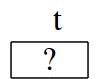
\includegraphics[scale=.5]{../img/java-tabl-repres2}\end{center}
  \item \java{t = new int[3];}
  \begin{center}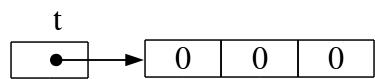
\includegraphics[scale=.5]{../img/java-tabl-repres1}\end{center}
 \end{itemize}
\end{frame}

\begin{frame}[fragile]{Repr�sentation}
  \emph{Exemple} : \java|int[][] t = new int[3][2];|
  \begin{itemize}
  \item Un tableau de 3 tableaux de 2 entiers
  \bigskip
  \begin{center}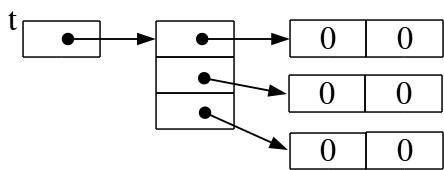
\includegraphics[scale=.4]{../img/java-tabl-dim2}\end{center}
  \item Repr�sentation interne $\not=$ vision classique
    \\
    \begin{small}
    \begin{center}\begin{tabular}{|c|c|}\hline ~ ~ 0 ~ ~ & ~ ~ 0 ~ ~ \\ \hline ~ ~ 0 ~ ~ & ~ ~ 0 ~ ~ \\ 
                                        \hline ~ ~ 0 ~ ~ & ~ ~ 0 ~ ~ \\ \hline\end{tabular}\end{center}
    \end{small}
 \end{itemize}
\end{frame}

\begin{frame}{Repr�sentation}
  Pour les tableaux � plusieurs dimensions
  \begin{itemize}
  \item Chaque �l�ment d'un tableau � deux dimensions est un tableau ind�pendant
  \item La taille ne fait pas partie du type
  \item $\Rightarrow$ Chaque �l�ment peut �tre d'une \emph{taille diff�rente}
  \end{itemize}
  \medskip
  \begin{center}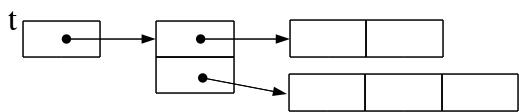
\includegraphics[scale=.5]{../img/java-tabl-dim2b}\end{center}
\end{frame}

\begin{frame}[fragile]{Cr�ation}
  On peut omettre les derni�res tailles
  \begin{itemize}
  \item Le tableau est cr�� en partie
  \item \emph{Exemple} :
  \begin{Java}
  int[][] t;
  t = new int[3][];
  \end{Java}
  \begin{center}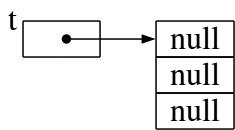
\includegraphics[scale=.5]{../img/java-tabl-new2}\end{center}
  \item Le reste sera cr�� plus tard
  \end{itemize}
\end{frame}

\begin{frame}[fragile]{Cr�ation}
  Cr�ation en donnant les valeurs
  \begin{grammaire}[fontsize=\footnotesize]
  \nterm{ArrayCreationExpression} :
   \term{new} \nterm{TypeName} \nterm{Dims} \nterm{ArrayInitializer}  

  \nterm{ArrayInitializer} :
     \term{\{} \nterm{VariableInitializers}\opt \term{,}\opt \term{\}}

  \nterm{VariableInitializers} :
     \nterm{VariableInitializer}
     \nterm{VariableInitializers} \term{,} \nterm{VariableInitializer}

  \nterm{VariableInitializer} :
     \nterm{Expression}
     \nterm{ArrayInitializer}
  \end{grammaire}
\end{frame}

\begin{frame}[fragile]{Cr�ation}
\emph{Exemple} de format long
  \begin{Java}
  int[] t1 = new int[] {4,5,6};
  int[] t2;
  t2 = new int[] {4,5,6};
  \end{Java}
\medskip
�criture abr�g�e (uniquement � la d�claration)
  \begin{Java}
int[] t2 = {4,5,6}; // �criture abr�g�e accept�e
int[] t3;
t3 = {4,5,6}; // Erreur � la compilation
  \end{Java}
\medskip
\emph{Exercice} : Donnez la repr�sentation m�moire
  \begin{itemize}
  \item \java|int[][] entierss = {{1,2},{3,4,5}};|
  \item \java|int[][] entierss = {{1,2},null};|
  \end{itemize}
\end{frame}

\begin{frame}[fragile]{Cr�ation}
  \emph{Exercice} : Les cr�ations suivantes sont-elles correctes ? Pourquoi ?
  \begin{itemize}
  \item \java|int[][] t = new int[2];|
  \item \java|int[][] t = new int[] {1,2};|
  \item \java|int[][] t = new int[] {{1},{2}};|
  \item \java|int[][] t = new int[3][2] {1,2};|
  \item \java|int[][] t = new int[3][2] {null,null};|
  \end{itemize}
\end{frame}

\begin{frame}[fragile]{Cr�ation}
\emph{Exercice} : Lecture d'un vecteur.
\\ Attention ! Ceci n'est pas correct. Pourquoi ?
\begin{Java}
  import java.util.Scanner;
  public class LectureVecteur {
     public static void main(String[] args) {
        Scanner clavier = new Scanner(System.in);
        int[] vecteur;    // le vecteur � lire
        int   taille;     // taille du vecteur
        taille = clavier.nextInt();
        for (int i=0; i<taille; i=i+1)
           vecteur[i] = clavier.nextInt();
     }
  }
\end{Java}
\end{frame}

\subsection{Taille}

\begin{frame}[fragile]{Taille}
La taille doit �tre un \java|int|
 \begin{itemize}
  \item Jusqu'� 2 milliards d'�l�ments ;-)
  \item Peut �tre \emph{nulle}
    \begin{itemize}
    \item ex : \java|int[][] t = new int[0][2];|
    \item peut avoir un sens comme cas limite
    \end{itemize}
  \item Ne peut \emph{pas} �tre \emph{n�gative}
    \begin{itemize}
    \item sinon une exception est lanc�e
    \item pas v�rifi� � la compilation m�me si constante
    \end{itemize}
  \item Est une expression g�n�rale
    \begin{itemize}
    \item ex : \java|int[] t2 = new int[clavier.nextInt()];|
    \end{itemize}
  \end{itemize}
\end{frame}

\begin{frame}[fragile]{Taille}
\emph{Rappel} : on connait la taille via \java|length|
\par\medskip Si plusieurs dimensions
    \begin{itemize}
    \item Taille (potentiellement) diff�rente d'une ligne � l'autre
    \item $\Rightarrow$ Sp�cifier la ligne
    \item Exemple :
      \begin{Java}
  int[][]t = {{1,2},{2,3,4}};
  System.out.println( "Nombre d'�l�ments = "
      + (t[0].length + t[1].length) );
      \end{Java}
    \end{itemize}
\end{frame}

\begin{frame}[fragile]{Taille}
\emph{Exemple} : Que va imprimer le code suivant?
\begin{Java}
  package be.heb.esi.lg1.tutorials.tableaux;

  public class ParcoursLigneParLigne{
     public static void main(String[] args){
        String[][] tableau= {{"00","01","02","03","04"},
                             {"10","11","12","13","14"}};
        for(int i = 0; i < tableau.length; i = i + 1)
           for(int j = 0; j < tableau.length; j = j + 1)
              System.out.println(tableau[i][j]);
     }
  }
\end{Java}
\end{frame}

\begin{frame}[fragile]{Taille}
\emph{Exemple} : Parcours d'un tableau d'entiers � deux dimensions ligne par ligne
\begin{Java}
  package be.heb.esi.lg1.tutorials.tableaux;

  public class ParcoursLigneParLigne{
     public static void main(String[] args){
        String[][] tableau= {{"00","01","02","03","04"},
                          {"10","11","12","13","14"}};
        for(int i = 0; i < tableau.length; i = i + 1)
           for(int j = 0; j < tableau[i].length; j = j + 1)
              System.out.println(tableau[i][j]);
     }
  }
\end{Java}
\end{frame}

\subsection{Parcours}

\begin{frame}[fragile]{foreach}
\emph{Rappel} : Le \emph{foreach} simplifie le parcours d'un vecteur
\begin{itemize}
\item[]
  \begin{Java}
  public static void afficher( int[] tab )  {
    for( int val : tab ) {
      System.out.print( val + " " );
    }
  }
  \end{Java}
\end{itemize}
\medskip
On peut l'utiliser pour une matrice
\begin{itemize}
\item version qui utilise le parcours d'un vecteur
\begin{Java}
  public static void afficher( int[][] mat )  {
    for( int[] ligne : mat ) {
      afficher( ligne );
      System.out.println();
    }
  }
\end{Java}
\end{itemize}
\end{frame}

\begin{frame}[fragile]{foreach}
\begin{itemize}
\item version qui refait tout
\begin{Java}
  public static void afficher( int[][] mat )  {
    for( int[] ligne : mat ) {
      for( int val : ligne ) {
        System.out.print( val + " " );
      }
      System.out.println();
    }
  }
\end{Java}
 \item Peut-on utiliser le \emph{foreach} pour un parcours \emph{colonne par colonne} ?
\end{itemize}
\end{frame}

\subsection{Assignation en bloc}

\begin{frame}[fragile]{Assignation}
  Un tableau est de type r�f�rence
  \begin{itemize}
  \item \emph{L'assignation} d'un tableau � un autre \emph{copie la r�f�rence} (et pas le tableau)
  \item Exemple : \java|int[] t1 = {4,5,6}, t2 = t1;|
  \medskip
  \begin{center}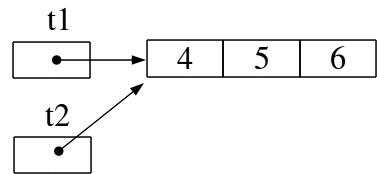
\includegraphics[scale=.5]{../img/java-tabl-ass1}\end{center}
  \end{itemize}
\end{frame}

\begin{frame}[fragile]{Assignation}
  \emph{Exemple} : \java|int[] t1 = {4,5,6}, t2 = {1,2}; t2 = t1;|
  \begin{center}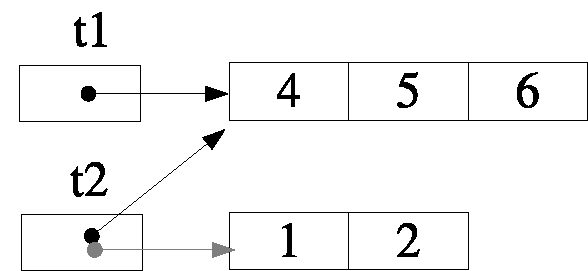
\includegraphics[scale=.7]{../img/java-tabl-ass2}\end{center}
  \begin{itemize}
  \item L'ancien tableau n'est plus r�f�renc�
  \item La place m�moire est r�cup�r�e (par le \textit{garbage collector})
  \end{itemize}
\end{frame}

\begin{frame}[fragile]{Acc�s aux �l�ments}
Pour acc�der � un �l�ment on donne tous les indices
      \\\emph{Exemple}
      \begin{Java}
  int[][][] t = new int[4][5][3];
  t[0][2][1] = 1; // Faites un sch�ma m�moire !
      \end{Java}
\bigskip
Cela a du sens de n'en sp�cifier que certains
      \\\emph{Exemple}
      \begin{Java}
  int[] t = { 4,5,6 };
  int[][] t2 = { {1,2,3}, {4,5} };
  t2[1] = t; // Faites un sch�ma m�moire !
      \end{Java}
\end{frame}

\begin{frame}[fragile]{Cr�ation}
\emph{Exemple} : Autre �criture pour la cr�ation d'un tableau.
\begin{Java}
  int[][] t = new int[3][2];
\end{Java}
Pourrait s'�crire
\begin{Java}
  int[][] t;
  t = new int[3][];
  for (int i=0; i<3; i=i+1)
     t[i] = new int[2];
\end{Java}
\end{frame}

\begin{frame}[fragile]{Cr�ation}
\emph{Exemple} : Cr�ation d'un tableau triangulaire
\begin{Java}
  package be.heb.esi.lg1.tutorials.tableaux;

  public class TableauTriangulaire{
     public static void main(String[] args){
        int[][] t;
        t = new int[3][];
        for (int i=0; i<3; i=i+1)
           t[i] = new int[i+1];
     }
  }
\end{Java}
\end{frame}

\begin{frame}[fragile]{Cr�ation}
\emph{Exemple} : Triangle de Pascal
\begin{Java}
  import java.util.Scanner;
  public class TrianglePascal {
     public static void main(String[] args) {
        Scanner clavier = new Scanner(System.in);
        int taille = clavier.nextInt();
        int[][] pascal; // le triangle de Pascal
        pascal = new int[taille][];
        for (int i=0; i<taille; i=i+1) {
           pascal[i] = new int[i+1];
           pascal[i][0] = 1;
           pascal[i][i] = 1;
           for(int j=1; j<i; j=j+1)
              pascal[i][j] = pascal[i-1][j-1]+pascal[i-1][j];
        }
     }
  }
\end{Java}
\end{frame}

\subsection{Erreurs et exceptions}

\begin{frame}[fragile]{Erreurs et exceptions}
Lors de l'acc�s � un �l�ment
\begin{itemize}
\item Si l'indice n'est pas valide (par rapport � la taille du tableau), 
la \sigle{JVM} lance une exception (\emph{ArrayIndexOutOfBoundException})
\item \emph{Exemple} :
\begin{Java}
  int[] entiers = {7,14,0};
  int i1 = entiers[-1]; // erreur � l'ex�cution
  int i2 = entiers[3]; // erreur � l'ex�cution
  int i3 = entiers[0.0]; // erreur � la compilation
\end{Java}
\end{itemize}
\end{frame}

\begin{frame}[fragile]{Erreurs et exceptions}
La \sigle{JVM} lance aussi une exception si le tableau est � \java|null| (\emph{NullPointerException})
\begin{itemize}
\item \emph{Exemple} :
\begin{Java}
  int[][] entierss = {{1,2},null};
  int[] entiers = entierss[1]; // OK
  int entier = entierss[1][0]; // erreur � l'ex�cution
\end{Java}
\end{itemize}
\end{frame}

\begin{frame}[fragile]{Erreurs et exceptions}
Lors d'une assignation
\begin{itemize}
\item Comme dans toute assignation, il faut que les \emph{types correspondent}
\item Exemple :
\begin{Java}
  int[] t1 = {4,5,6};
  boolean[] t2 = t1; // erreur � la compilation
\end{Java}
\item \emph{Exemple} :
\begin{Java}
  int[][] t1 = {{4,5,6},{1,2}};
  int[] t2 = t1[0]; // t2={4,5,6};
\end{Java}
\end{itemize}
\end{frame}

\subsection{Tableau et m�thode}

\begin{frame}[fragile]{M�thode}
Passer un tableau en param�tre
\\= Passer une copie de la r�f�rence au tableau
\begin{itemize}
\item La m�thode agit sur le tableau et pas une copie
\end{itemize}
\medskip
\emph{Exemple} : Un tableau en argument
\begin{itemize}
\item[]
\begin{Java}
  public class TableauEnArgument {
     public static void iniTableau(int[] tab) {
        for(int i=0; i<tab.length; i++)
           tab[i]=0;
     }

     public static void afficheTab(int[] tab) {
        for(int i=0; i<tab.length; i++)
           System.out.print(tab[i]+" ");
     }
  }
\end{Java}
\end{itemize}
\end{frame}

\begin{frame}[fragile]{M�thode}
\emph{Exemple} : Utilisation
\begin{itemize}
\item[]
\begin{Java}
  public class Test {
     public static void main(String[] args) {
        int[] tableau = new int[]{8,4,3,9};
        System.out.print("tableau avant: ");
        TableauEnArgument.afficheTab(tableau);
        TableauEnArgument.iniTableau(tableau);
        System.out.print("\ntableau apr�s: ");
        TableauEnArgument.afficheTab(tableau);
    }
  }
\end{Java}
\end{itemize}
\end{frame}

\begin{frame}[fragile]{M�thode}
\emph{Exemple} : Un tableau en retour
\begin{itemize}
\item[]
\begin{Java}
  public static int[] tableauEnRetour(int n) {
     int[] tableau = new int[n];
     for(int i=0;i<n;i++)
        tableau[i]=i+1;
     return tableau;
  }
\end{Java}
\item Un appel de la m�thode \emph{tableauEnRetour} fournira une r�f�rence � un tableau
\item Il est possible de modifier les valeurs des �l�ments
\end{itemize}
\end{frame}

\begin{frame}[fragile]{M�thode principale}
La m�thode \java|main| re�oit un tableau en argument
\begin{Java}
  public static void main(String[] args)
\end{Java}
\begin{itemize}
\item Il s'agit d'\emph{arguments} fournis au programme
\item \emph{Comment ?} via la ligne de commande
\begin{Java}
  java Test mes arguments
\end{Java}
\item Arguments s�par�s par un (des) espace(s)
\end{itemize}
\end{frame}

\begin{frame}[fragile]{M�thode principale}
\emph{Exemple} :
\begin{Java}
  public class Miroir {
    public static void main(String[] args) {
      System.out.print(args.length + ": ");
      for(int i=args.length-1; i>=0; i--)
        System.out.print(args[i] + " ");
    }
  }
\end{Java}
\begin{Code}
  > java Miroir Un message � l'envers
  4: l'envers � message Un 
\end{Code} 
\begin{Java}
  > java Miroir "Un message � l'envers"
  1: Un message � l'envers 
\end{Java} 
\end{frame}

\begin{frame}{Arrays}
La classe \emph{Arrays} offre des outils pratiques
\begin{itemize}
\item \emph{equals} : teste l'�galit� de tableaux
\item \emph{fill} : remplit tout un tableau avec une m�me valeur
\item \emph{toString} : retourne une chaine reprenant les �l�ments du tableau
\item \emph{copyOf}, \emph{sort}, \dots
\end{itemize}
\end{frame}



% ====== Second quadrimestre
%=== Cours de Java
%=== Chapitre : OO

\section{L'orient� objet}

\begin{frame}
\begin{block}{\center Le�on \thesection\ ---   \insertsection}
  {
  \begin{multicols}{2}
  \tableofcontents[sectionstyle=hide,subsectionstyle=show/show/hide]
  \end{multicols}
  \bigskip
  }
\end{block}
\end{frame}

\begin{frame}{Avertissement}
Pour qu'un langage soit \textit{orient� objet} il doit poss�der 3 propri�t�s
  \begin{itemize}
  \item L' \emph{encapsulation}
  \item L' \emph{h�ritage}
  \item Le \emph{polymorphisme}
  \end{itemize} 
\bigskip
Trop pour le cours de 1�re ann�e
  \begin{itemize}
  \item Nous allons surtout voir l'encapsulation \\(comme au cours de logique)
  \item Et effleurer le reste $\longrightarrow$ parfois impr�cis
  \end{itemize}
\end{frame}

\begin{frame}{Rappels}
Voici ce que vous avez d�j� vu en logique
\begin{center}
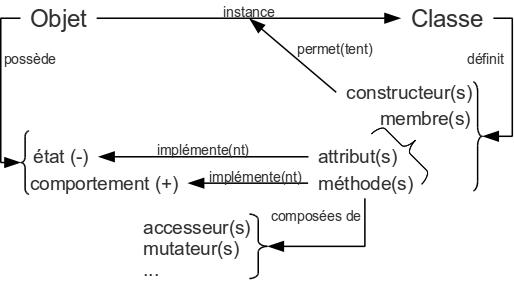
\includegraphics[scale=.6]{../img/oo-rappels}
\end{center}
\end{frame}

\begin{frame}{Pr�sentation de l'exemple}
Illustrons ces concepts avec la notion d'\textit{�tudiant � l'ESI}
\begin{itemize}
 \item Un �tudiant
    \begin{itemize}
    \item poss�de un nom et un num�ro unique
    \item est inscrit dans une ann�e d'�tude
    \item est doubleur ou pas
    \item est un \textit{ancien} (a termin�) ou pas
    \end{itemize}
  \item Il peut r�ussir son ann�e ou la rater
  \end{itemize}
\end{frame}

\subsection{La classe}

\begin{frame}{La classe}
  \emph{Exemple}: Repr�sentation graphique (UML) de la classe \textit{Etudiant}
  \begin{center}
  \begin{tabular}{cl}
    {\small\fcolorbox{black}{bleu}{
      \begin{tabular}{l}
        ~~~~~~~~~Etudiant\\ 
        \hline
        - num�ro : Entier\\
        - nom : Chaine\\
        - ann�eEtude : Entier\\
        - doubleur : Bool�en\\
        - ancien : Bool�en\\
        \hline
        + aR�ussi()\\
        + aRat�()\\
      \end{tabular}
    }} &
    {\small
      \begin{tabular}{l}
        \textbf{Nom de la classe} \\ 
        \textbf{Attributs} \\
        Le "-" indique qu'ils sont \textbf{priv�s}\\
        Connus uniquement dans la classe\\
        En \sigle{Java} on �crira \java|private|\\
        \\
        \textbf{M�thodes}\\
        Le "+" car elles sont \textbf{publiques}\\
        En \sigle{Java} on �crira \java|public|\\
      \end{tabular}
    } \\
  \end{tabular}
  \end{center}
\end{frame}

\subsection{Les objets}

\begin{frame}{Les objets}
  \emph{Exemple} : Repr�sentation graphique de 2 objets (instances) possibles :
  \medskip
  \begin{center}
  \begin{tabular}{cc}
  {\small\fcolorbox{black}{bleu}{
    \begin{tabular}{l}
      \underline{James Gosling}: Etudiant\\ 
      \hline
      - num�ro = 34000\\
      - nom = "James Gosling"\\
      - ann�eEtude = 1\\
      - doubleur = faux\\
      - ancien = faux\\
      \hline
      + aR�ussi()\\
      + aRat�()\\
    \end{tabular}
  }} &
  {\small\fcolorbox{black}{bleu}{
    \begin{tabular}{l}
      \underline{Ada Lovelace}: Etudiant\\ 
      \hline
      - num�ro = 33800\\
      - nom = "Ada Lovelace"\\
      - ann�eEtude = 2\\
      - doubleur = faux\\
      - ancien = faux\\
      \hline
      + aR�ussi()\\
      + aRat�()\\
    \end{tabular}
  }} \\
  \end{tabular}
  \end{center}
\end{frame}

\subsection{Les membres}

\begin{frame}{Les membres}
Chaque instance poss�de les m�mes attributs mais avec des \emph{valeurs diff�rentes}
\\\bigskip
Les m�thodes d'une instance agissent sur les attributs de cette instance 
  \begin{itemize}
   \item La m�thode \textit{aRat�()} d'un �tudiant va mettre \emph{son} attribut \textit{doubleur} � vrai
   \item Que ferait la m�thode \textit{aR�ussi()} ?
  \end{itemize}
\end{frame}

\begin{frame}[fragile]{La classe en Java}
  � ce stade la classe \texttt{Etudiant} peut s'�crire :
  \begin{multicols}{2}  
  \begin{Java}
  public class Etudiant {

    private int num�ro; 
    private String nom;
    private int ann�eEtude;
    private boolean doubleur;
    private boolean ancien; 

    public void aRat�() {
      doubleur = true;
    }
  \end{Java}
  \begin{Java}

    public void aR�ussi() {
      doubleur = false;
      ann�eEtude++;
      if (ann�eEtude == 4 ) {
        ancien = true;
      }
    }

  }  
  \end{Java}
  \end{multicols}
\begin{itemize}
\item Remarquez l'absence de \java{static} pour les m�thodes
\end{itemize}
\end{frame}

\begin{frame}{OO or not OO ?}
On utilisait d�j� \java|class|. On faisait de l'objet ?
\\\bigskip
Oui et non ;)
\begin{itemize}
\item \sigle{Java} est un langage orient� objet
\item Mais il permet une �criture non OO
\item Via l'utilisation de \java|static|
(qui a un sens plus large que nous d�taillerons plus loin)
\end{itemize}
\end{frame}

\begin{frame}{OO or not OO ?}
En gros, on a 2 sortes de classes : 
\\\bigskip
\begin{small}
\begin{tabular}{l|l|l}
\hline\hline
& {\small \emph{approche non OO}} & {\small \emph{approche OO}} \\\hline
But & regrouper des m�thodes & d�finir un type de donn�es \\
Attribut & non (sauf constantes) & oui \\
Instances & non & oui \\
Utilisation via & le nom de la classe & une instance \\
\java|static| & oui & non \\
Fr�quence & rare & fr�quent \\
Exemples & \java|Math| & \java|String|, \java|Scanner| \\
\hline\hline
\end{tabular}
\end{small}
\\\bigskip
\textit{En pratique, on rencontrera des situations mixtes}
\end{frame}

\begin{frame}{Visibilit� des membres}
En \sigle{Java} : 4 visibilit�s
\begin{description}
  \item[public] : visible dans \textbf{toutes} les classes (\java|public|)
  \item[priv�] : n'est accessible que de \textbf{la} classe (\java|private|)
  \item[<<paquet�>>] : visible dans toutes les classes du \textit{package} (pas de mot cl�)
  \item[prot�g�] : pas vu en 1�re ann�e (\java|protected|)
\end{description}
\bigskip
Rappel \emph{bonne pratique} :
\\attributs priv�s / m�thodes publiques
\end{frame}

\subsection{Constructeur}

\begin{frame}[fragile]{Constructeur}
\emph{Exemple} : D�finition d'un constructeur
  \begin{Java}
  public Etudiant (int unNum�ro, String unNom) {
    num�ro = unNum�ro;
    nom = unNom;
    ann�eEtude = 1;
    doubleur = false;
    ancien = false;
  }
  \end{Java}
  Ressemble � une m�thode mais
  \begin{itemize}
    \item Pas de type de retour d�clar�
%    \item En pratique, retourne la r�f�rence de l'objet 
    \item A le m�me nom que celui de la classe
  \end{itemize}
\end{frame}

\subsection{Instanciation}

\begin{frame}[fragile]{Instanciation}
Pour instancier 
\begin{itemize}
\item On utilise l'op�rateur \java|new|
\item On fournit les param�tres au constructeur
\end{itemize}
\medskip
\emph{Exemple} : instanciation d'un �tudiant
\begin{itemize}
\item[]
\begin{Java}
Etudiant ada = new Etudiant(33800, "Ada Lovelace");
\end{Java}
\item Cr�e un nouvel objet \java|Etudiant|
\item Appelle le constructeur pour l'initialiser
\end{itemize}
\end{frame}

\begin{frame}[fragile]{Instanciation}
Une classe est un type \emph{r�f�rence} (comme les tableaux)
\medskip
\\\emph{Exemple} :
\begin{Java}
    Etudiant ada;  // r�f�rence cr��e sur la pile
\end{Java}
\vspace{-10pt}
\begin{center}
\includegraphics[scale=.4]{../img/java-oo-alloc1}\end{center}
\begin{Java}
    ada = new Etudiant(33800,"Ada Lovelace"); // objet cr�� sur le tas
\end{Java}
\vspace{-10pt}
\begin{center}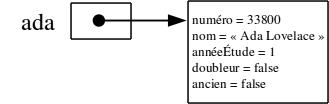
\includegraphics[scale=.5]{../img/java-oo-alloc2}\end{center}
\end{frame}

\begin{frame}[fragile]{Appel d'une m�thode}
Utilisation de la notation \textit{point�e} (op�rateur \code{.})
\\\bigskip
\emph{Exemple}
\begin{Java}
public static void main(String[] args) {
    Etudiant ada = new Etudiant(33800, "Ada Lovelace");
    ada.aR�ussi();
}
\end{Java}
\bigskip
Code que l'on peut trouver
\begin{itemize}
\item dans une autre classe
\item dans la classe m�me
\end{itemize}
\end{frame}

\subsection{Accesseurs}

\begin{frame}[fragile]{Accesseurs}
\emph{Accesseur} : m�thode donnant la valeur d'un attribut 
\\\bigskip
\emph{Exemple} : pour notre classe �tudiant
\begin{Java}
  public int getNum�ro() {return num�ro;}
  public String getNom() {return nom;}
  public int getAnn�eEtude() {return ann�eEtude;}
  public boolean isDoubleur() {return doubleur;}
  public boolean isAncien() {return ancien;}
\end{Java}
\bigskip
Par convention, l'accesseur de \java|attribut| est \java|getAttribut| 
(\java|isAttribut| pour un bool�en)
\end{frame}

\begin{frame}[fragile]{Appel d'une m�thode}
\emph{Exemple} : Utilisation des accesseurs
\begin{Java}
public static void main(String[] args) {
    Etudiant ada = new Etudiant(33800, "Ada Lovelace");
    System.out.println(ada.getAnn�eEtude()); // 1
    ada.aR�ussi();
    System.out.println(ada.getAnn�eEtude()); // 2
    System.out.println(ada.isDoubleur()); // false
    ada.aRat�();
    System.out.println(ada.getAnn�eEtude()); // 2
    System.out.println(ada.isDoubleur()); // true
}
\end{Java}
\end{frame}

\subsection{Mutateurs}

\begin{frame}[fragile]{Mutateurs}
\emph{Mutateur} : sert � modifier un attribut 
\\\bigskip
\emph{Exemple} : un mutateur possible pour \textit{Etudiant}
\begin{Java}
  public void setNom(String unNom) {nom = unNom;}
\end{Java}
\bigskip
Par convention, le mutateur de \java|attribut| est \java|setAttribut|
\\\bigskip
\emph{Exemple} : Appel d'un mutateur
\begin{Java}
  Etudiant ada = new Etudiant(33800,"Ada Lovelace");
  System.out.println( ada.getNom() );
  ada.setNom("James Gosling");
  System.out.println( ada.getNom() );
\end{Java}
\end{frame}

\begin{frame}{Mutateurs}
\emph{Bonne pratique} : 
\\Bien r�fl�chir avant de fournir un mutateur
\begin{itemize} 
\item Est-ce que le num�ro peut changer ? Non !
\item Est-ce que le nom peut changer ? Euh !
\item Est-ce que l'ann�e peut changer ? Oui ! 
  \begin{itemize} 
  \item Mais est-ce qu'il faut permettre de la changer directement ?
  \item ou uniquement via des m�thodes comme \java|aR�ussi()| ? 
  \\� voir au cas par cas
  \end{itemize}
\end{itemize}
\end{frame}

\begin{frame}[fragile]{Tests de validit�}
Il est conseill� d'effectuer des \emph{tests de validit�} sur les param�tres
\begin{itemize}
\item Constructeur : objet cr�� dans un �tat valide
\item Mutateur : l'�tat reste valide
\end{itemize}
\emph{Exemple} :
\begin{Java}
  public void setNum�ro(int unNum�ro) {
    if (unNum�ro<=0) {
      throw new IllegalArgumentException("Le num�ro est n�gatif !");
    }
    num�ro = unNum�ro;
  }
\end{Java}
\end{frame}

%\begin{frame}[fragile]{Tests de validit�}
%\emph{Bonne pratique} :
%\\Appeler les mutateurs dans le constructeur
%\begin{itemize} 
%  \item On �vite ainsi de dupliquer les tests
%  \item Exemple
%\begin{Java}
%  public Etudiant (int unNum�ro, String unNom) {
%    setnum�ro(unNum�ro);
%    // la suite...
%}
%\end{Java}
%\item Et si un test est n�cessaire mais qu'on ne veut pas offrir de mutateur ? D�finir le mutateur en priv�
%\end{itemize}
%\end{frame}

\subsection{Surcharge}

\begin{frame}{Surcharge}
\emph{Surcharge} (overloading) : possibilit� de d�finir plusieurs m�thodes/constructeurs
\begin{itemize}
\item De m�me nom
\item Si signatures diff�rentes
\item Facilit� pour l'utilisateur
\end{itemize}
\bigskip
Tr�s utile pour les constructeurs
\begin{itemize}
\item Plusieurs fa�ons d'initialiser l'�tat
\end{itemize}
\end{frame}

\begin{frame}[fragile]{Surcharge}
\emph{Exemple} : Constructeurs pour \texttt{Etudiant}
\begin{Java}
  public Etudiant (int unNum�ro, String unNom) {
    num�ro = unNum�ro;
    nom = unNom;
    ann�eEtude = 1;
    doubleur = false;
    ancien = false;
  }

  public Etudiant (int unNum�ro, String unNom, int ann�e, 
                   boolean doubl, boolean anc) {
    num�ro = unNum�ro;
    nom = unNom;
    ann�eEtude = ann�e;
    doubleur = doubl;
    ancien = anc;
  }
\end{Java}
\end{frame}

\subsection{this}

\begin{frame}[fragile]{this()}
Souvent, les constructeurs d'une m�me classe se ressemblent
  \begin{itemize}
  \item Cf. exemple pr�c�dent
  \item Plus facile si un constructeur appelle l'autre
  \item On utilise la notation \java|this()|
  \item Exemple
  \begin{Java}
  public Etudiant (int num�ro, String nom) {
    this(num�ro, nom, 1, false, false);
  }
  \end{Java}
  \item Doit �tre la \emph{premi�re instruction}
  \end{itemize}
\end{frame}

\begin{frame}[fragile]{Le mot cl� <<this>>}
Le mot cl� \java{this} est une r�f�rence � soi-m�me 
\begin{itemize}
\item Implicite lors d'une utilisation directe du membre
\item \emph{Exemple}
  \begin{Java}
  public void setNom( String unNom ) {
    nom = unNom;  // implicitement: this.nom = unNom;
  }

  public void aR�ussi() {
    f�liciter(); // implicitement : this.f�liciter();
    // ...
  }

  public void f�liciter() {
    // ...
  }
  \end{Java}
\end{itemize}
\end{frame}

\begin{frame}[fragile]{Le mot cl� <<this>>}
R�gle : un param�tre/une variable locale \emph{masque} un attribut
  \begin{itemize}
  \item \java|this| permet d'acc�der � l'attribut masqu� 
  \item \emph{Exemple}
  \begin{Java}
  public void setNom( String nom ) {
    this.nom = nom;
  }
  \end{Java}
  \item Certains l'utilisent syst�matiquement pour une meilleure lisibilit�
  \end{itemize}
\end{frame}

\subsection{static}

\begin{frame}{Comprendre <<static>>}
  \emph{\java{static}} s'applique aux membres (attributs + m�thodes)
  \begin{itemize}
    \item N'est plus un membre de l'objet (instance de la classe) mais un membre de la classe
    \item Est \emph{partag�} par toutes les instances
  \end{itemize}
\end{frame}

\begin{frame}[fragile]{Comprendre <<static>>}
  \emph{Attribut} statique
  \begin{itemize}
    \item Existe en un seul exemplaire 
    \item Est initialis� lors du chargement de la classe \\(une seule fois)
    \item Utilisation courante : constantes
  \\\emph{Exemple}
  \begin{Java}
  public class Board {
    public static final int NB_LIGNES = 8;
    public static final int NB_COLONNES = 7;
  }
  \end{Java}
  \end{itemize}
\end{frame}

\begin{frame}[fragile]{Comprendre <<static>>}
  \emph{M�thode} statique
  \begin{itemize}
    \item Ne peut pas acc�der aux membres des instances
    \item Utilisation courante : m�thodes non objets
  \\\emph{Exemple}
  \begin{Java}
  public class Outils {
    public static int abs(int nb) {
      return nb < 0 ? -nb : nb;
    }
  }
  \end{Java}
  \end{itemize}
\end{frame}

\begin{frame}[fragile]{Comprendre <<static>>}
  � l'ext�rieur de la classe, 
  \begin{itemize}
  \item on pr�fixe par le nom de la classe
  \begin{Java}
  int abs = Outils.abs(-3);
  int lg = Board.NB_LIGNES;
  double un = Math.log (Math.E);
  \end{Java}
  \item ou un objet de la classe (non recommand�)
  \begin{Java}
  int lg = monBoard.NB_LIGNES;
  \end{Java}
  \end{itemize}
\end{frame}

\begin{frame}[fragile]{Comprendre <<static>>}
  \java{import static} cr�e un raccourci pour l'acc�s aux membres statiques 
  \\\bigskip\emph{Exemple}
  \begin{Java}
  import static java.lang.Math.log;
  import static java.lang.Math.E;
  public class Test {
    public static void main( String[] args ) {
      System.out.println( log(E) );
    }
  }
  \end{Java}
\end{frame}

\begin{frame}[fragile]{Un mot sur les structures}
En Logique, vous avez vu le concept de structure
\begin{itemize}
\item On peut imiter cette construction
\item \emph{Exemple} : une structure Adresse
\vspace{-0.5cm}
\begin{multicols}{2}
\begin{Code}
structure Adresse compos�e de
    rue : chaine
    num�ro : chaine
    code : entier
   localit� : chaine
fin structure
\end{Code}
\begin{Java}
public class Adresse {
    public String rue;
    public String num�ro;
    public int    code;
    public String localit�;
}
\end{Java}
\end{multicols}
\vspace{-0.5cm}
\item Mais, on pr�f�re une classe normale qui permet de contr�ler la valeur des champs
\end{itemize}
\end{frame}

\begin{frame}{Pr�cision sur l'instanciation}
Attributs initialis�s � une \emph{valeur par d�faut} \\(comme pour les tableaux)
  \begin{itemize}
  \item Num�rique : \java|0|
  \item Bool�en : \java|false|
  \item r�f�rence : \java|null| (r�f�rence vers \emph{rien})
  \end{itemize}
\bigskip
Rarement ce qui est souhait�
  \\$\longrightarrow$ toujours donner des valeurs explicites
\end{frame}

\begin{frame}{Pr�cision sur les constructeurs}
Il existe un \emph{constructeur par d�faut}
\begin{itemize}
  \item sans param�tre 
  \item ne fait rien
  \item uniquement \emph{si pas de constructeur explicite}
  \item Rarement une bonne id�e 
\end{itemize}
$\longrightarrow$ toujours �crire explicitement un constructeur
\end{frame}

\subsection{Des objets comme attributs}

\begin{frame}[fragile]{Des objets comme attributs}
Une classe d�finit un type � part enti�re 
\\$\longrightarrow$ peut �tre attribut d'une autre classe
  \begin{itemize}
  \item \emph{Ex} : \texttt{String} pour le nom d'un �tudiant
  \item \emph{Ex} : \texttt{Date} (de naissance) d'un �tudiant
  \end{itemize}
\bigskip
\pause
\emph{Exemple} : D�finissons le concept d'adresse
\begin{Java}[basicstyle=\scriptsize]
public class Adresse {
  private String rue;
  private String num�ro;
  private int codePostal;
  private String localit�;
  
  public Adresse (String uneRue, String unNum�ro, 
          int unCodePostal, String unelocalit�) {
    // ...
  }
  // + accesseurs 
  // pas de mutateur ! Pourquoi ?
}
\end{Java}
\end{frame}

\begin{frame}[fragile]{Des objets comme attributs}
\emph{Exemple} : Ajoutons une adresse � un �tudiant
\begin{Java}
public class Etudiant {
  private Adresse adresse;
  
  public Etudiant (int unNum�ro, String unNom, Adresse uneAdresse) {
    adresse = uneAdresse;
    // ...
  }

  public Adresse getAdressse() {return adresse;}

  public void setAdresse(Adresse uneAdresse) {
    adresse = uneAdresse;
  }
  // ... 
}
\end{Java}
\end{frame}

\begin{frame}[fragile]{Des objets comme attributs}
\emph{Exemple} : Cr�ons un �tudiant
\begin{Java}
 Adresse adresse = new Adresse("Rue Royale", "67", 1000, "Bruxelles");
 Etudiant james = new Etudiant( 34000, "James Gosling", adresse );
\end{Java}
ou, en condens�
\begin{Java}
  Etudiant james = new Etudiant ( 
                       34000, "James Gosling", 
                       new Adresse("Rue Royale", "67", 1000, "Bruxelles") 
           );
\end{Java}
\end{frame}

\subsection{Objets et tableaux}

\begin{frame}[fragile]{Des tableaux d'objets}
Une classe d�finit un type de donn�es 
\\$\longrightarrow$ on peut d�finir des tableaux d'objets
\\\bigskip
\emph{Exemple} : un tableau d'�tudiants \java|Etudiant[]|
\begin{Java}
// Affiche un tableau d'�tudiants
public static void afficher(Etudiant[] �tudiants) {
    System.out.println("Il y a " + �tudiants.length + " �tudiants");
    for( Etudiant �tudiant : �tudiants ) {
        System.out.println( �tudiant );
    }
}
\end{Java}
\end{frame}

\begin{frame}[fragile]{Des tableaux d'objets}
\begin{Java}
// Faire r�ussir tous les �tudiants
public static void tourn�eG�n�rale(Etudiant[] �tudiants) {
    // Faire un sch�ma pour comprendre que le foreach est correct
    for( Etudiant �tudiant : �tudiants ) {
        �tudiant.aR�ussi();
    }
}
\end{Java}
\begin{Java}
  // Test
  Etudiant[] groupe11 = {
      new Etudiant("20000", "Tintin"),
      new Etudiant("20001", "Milou"),
      new Etudiant("20002", "Professeur Tournesol"),
      new Etudiant("20003", "Capitaine Haddock");
  };
  afficher(groupe11);
  tourn�eG�n�rale(groupe11);
  afficher(groupe11);
\end{Java}
\end{frame}

\begin{frame}{Des tableaux \textbf{dans} les objets}
Un tableau d�finit un type de donn�es
\\$\longrightarrow$ on peut le trouver comme attribut
\\\bigskip
\emph{Exemple} : D�finissons, la classe Groupe (d'�tudiants)
\begin{itemize}
\item La taille (maximale) du groupe sera donn�e � la construction
\item Une m�thode permet d'ajouter un �tudiant au groupe
\end{itemize}
\end{frame}

\begin{frame}[fragile]{Des tableaux \textbf{dans} les objets}
\begin{Java}
public class Groupe {
    private Etudiant[] �tudiants;
    private int nbEtudiants;

    public Groupe(int taille) {
        if (taille < 1)
          throw new IllegalArgumentException("Pas de groupe vide");
        �tudiants = new Etudiant[taille]; // Faire un sch�ma !
        nbEtudiants = 0;
    } 

    public void ajouter(Etudiant �tudiant) {
        if (nbEtudiants == �tudiants.length)
          throw new IllegalStateException("Plus de place !");
        �tudiants[nbEtudiants] = �tudiant;
        nbEtudiants++;
    }
    // ...
\end{Java}
\end{frame}

\begin{frame}[fragile]{Des tableaux \textbf{dans} les objets}
\begin{Java}
    public void afficher() {
        System.out.println("Il y a " + nbEtudiants + " �tudiants");
        // Pourquoi pas un foreach ?
        for( int i=0; i<nbEtudiants; i++ ) {
            System.out.println( �tudiants[i] );
    }
    
    // On pourrait encore d�finir beaucoup de m�thodes utiles
}
\end{Java}
\begin{Java}
  // Test
  Groupe groupe11 = new Groupe(10);
  groupe11.ajouter(new Etudiant("20000", "Tintin"));
  groupe11.ajouter(new Etudiant("20001", "Milou"));
  groupe11.ajouter(new Etudiant("20002", "Professeur Tournesol"));
  groupe11.ajouter(new Etudiant("20003", "Capitaine Haddock"));
  groupe11.afficher();
\end{Java}
\end{frame}

\begin{frame}{Rappel}
Pour qu'un langage soit \textit{orient� objet} il doit poss�der 3 propri�t�s
  \begin{itemize}
  \item L' \emph{encapsulation}
  \item L' \emph{h�ritage}
  \item Le \emph{polymorphisme}
  \end{itemize} 
\bigskip
Nous avons vu l'encapsulation; survolons le reste
\end{frame}

\begin{frame}{H�ritage}
\emph{H�ritage} : Permet de d�finir une classe � partir d'une autre
\begin{itemize}
\item Un peu comme du \textit{copier-coller}
\item On r�cup�re ainsi tous les attributs et toutes les m�thodes
\item Terminologie
  \begin{itemize}
  \item Classe \emph{parent} : celle dont on h�rite
  \item Classe \emph{enfant} : celle qui h�rite
  \end{itemize} 
\end{itemize} 
\end{frame}

\subsection{H�ritage}

\begin{frame}{H�ritage}
\begin{itemize}
\item Graphiquement, on le note ainsi
\begin{center}
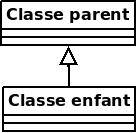
\includegraphics[scale=.5]{../img/oo-heritage}
\end{center}
\item L'h�ritage peut se lire dans la javadoc
\item Par d�faut, on h�rite de la classe \java|Object| 
\end{itemize} 
\end{frame}

\subsection{Object}

\begin{frame}{Object}
  Que trouve-t-on dans \java|Object| ? (cf. API)
\medskip
  \begin{itemize}
  \item \java{String toString()}
    \begin{itemize}
    \item Repr�sentation textuelle de (l'�tat de) l'objet
    \item Surtout � des fins de \emph{d�verminage}  
    \item Appel�e implicitement par \java|println|
    \end{itemize}
\medskip
  \item \java{boolean equals(Object o)}
    \begin{itemize}
    \item Compare 2 objets
    \end{itemize}
  \end{itemize}
\end{frame}

\begin{frame}{Overriding}
Java permet la r��criture (\emph{overriding}) d'une m�thode dans une classe enfant
\begin{itemize}
  \item Le travail fait par la m�thode dans la classe parent ne convient plus dans la classe enfant, je r�cris la m�thode
\end{itemize}
\textbf{Remarque}
\begin{itemize}
  \item � ne pas confondre avec l'\emph{overloading} (la surcharge) d'une m�thode
\end{itemize}
\end{frame}

\subsection{Repr�sentation textuelle}

\begin{frame}[fragile]{Repr�sentation textuelle}
Par d�faut, l'affichage d'un objet est peu clair
\\(utilisation de la version de \java|toString| h�rit�e d'\java|Object|)
\\\bigskip
\emph{Exemple} :
  \begin{itemize}
  \item[]
  \begin{Java}
  Etudiant ada = new Etudiant(33800, "Ada Lovelace");
  System.out.println(ada);
  \end{Java}
  \item[]affiche
  \item[]
  \begin{Java}
  be.heb.esi.java1.Etudiant@19189e
  \end{Java}
  \end{itemize}
\end{frame}

\begin{frame}[fragile]{Repr�sentation textuelle}
On peut red�finir la m�thode \java|toString|
\\\bigskip
\emph{Exemple} :
\begin{Java}
  public String toString () {
    String res = "(" + nom + ", " + num�ro;
    if (ancien) {
        res = res + ", ancien";
    } else {
        res = res + ", " + ann�eEtude;
        if (doubleur) { 
            res = res + ", doubleur";
        }
    }
    res = res + ")";
    return res;
  }
\end{Java}
\end{frame}

\begin{frame}[fragile]{Repr�sentation textuelle}
L'affichage est � pr�sent plus clair
\\\bigskip
\emph{Exemple} :
  \begin{itemize}
  \item[]
  \begin{Java}
  Etudiant ada = new Etudiant(33800, "Ada Lovelace");
  System.out.println(ada);
  ada.aR�ussi(); 
  System.out.println(ada);
  \end{Java}
  \item[] affiche
  \item[]
  \begin{Java}
  (Lovelace,33800,1)
  (Lovelace,33800,2)
  \end{Java}
  \end{itemize}
\end{frame}

\subsection{La m�thode equals()}

\begin{frame}[fragile]{La m�thode equals()}
Les objets sont des types r�f�rences
\\$\longrightarrow$ l'op�rateur \java|==| teste si c'est le \emph{m�me} objet
\\\bigskip
\emph{Exemple}
\begin{Java}
  Etudiant ada = new Etudiant(33800, "Ada Lovelace");
  Etudiant ada2 = new Etudiant(33800, "Ada Lovelace");
  System.out.println( ada == ada2 );  // false
\end{Java}
\bigskip
La m�thode \java|equals| permet de tester
\begin{itemize}
\item que les 2 objets sont dans le \emph{m�me �tat}  
\item m�me si c'est dupliqu� en m�moire
\end{itemize}
\end{frame}

\begin{frame}{La m�thode equals()}
La m�thode par d�faut dans \java|Object| se contente de comparer les r�f�rences
$\longrightarrow$ besoin de la r�crire
\begin{itemize}
\item Il faut respecter la signature
\item Doit r�pondre \og faux\fg\ si on compare � autre chose qu'un �tudiant (ou \java|null|)
\end{itemize}
\medskip
\emph{Exemple} : Red�finissons l'�galit� pour les �tudiants
\end{frame}

\subsection{Polymorphisme}

\begin{frame}[fragile]{Le polymorphisme}
La signature de la m�thode \java|equals| peut surprendre 
\begin{Java}
  public boolean equals(Object o) { // ...
\end{Java}
\begin{itemize}
\item Elle attend un \java|Object| en param�tre
\item On peut lui passer un \java|Etudiant|
\item C'est gr�ce au polymorphisme
\end{itemize}
\medskip
\emph{Polymorphisme} : L� o� on attend un objet d'une classe \og parent\fg\ on peut donner un objet
d'une classe \og enfant\fg\
\end{frame}

\begin{frame}[fragile]{Le polymorphisme}
Si on peut recevoir n'importe quelle sorte d'objet, comment savoir ce qu'on re�oit vraiment ?
\\\medskip
Gr�ce � l'op�rateur \java|instanceof|
\begin{itemize}
\item Dit si un objet appartient � une classe donn�e \\(ou un de ses enfants)
\item Par d�finition, \java|null| n'est instance de rien
\end{itemize}
\medskip
Notre m�thode \java|equals| devient
\begin{Java}
  public boolean equals(Object o) {
    if ( ! (o instanceof Etudiant) ) return false;
    // ...
\end{Java}
\end{frame}

\begin{frame}{Le polymorphisme}
Le \emph{casting}
\begin{itemize}
\item Nous savons que \java|o| est un �tudiant \\(puisque nous faisons le test juste avant)
\item Le compilateur, lui, ne le sait pas
\item Le compilateur se base sur la d�claration et consid�re \java|o| comme un \java|Object|
\item Il refuserait d�s lors l'appel de m�thodes propres � un \java|Etudiant|
\item Le \emph{casting} \java|(Classe)| demande au compilateur de voir l'objet comme le type enfant
\end{itemize}
\end{frame}

\begin{frame}[fragile]{La m�thode equals()}
Au final, on a
\begin{Java}
  public boolean equals(Object o) {
    if ( ! (o instanceof Etudiant) ) return false;
    Etudiant autre = (Etudiant) o;
    return this.num�ro ==  autre.num�ro 
        && this.nom.equals(autre.nom)
        && this.ann�eEtude == autre.ann�eEtude
        && this.doubleur == autre.doubleur
        && this.ancien == autre.ancien;
  }
\end{Java}
\begin{Java}
  Etudiant ada = new Etudiant(33800, "Ada Lovelace");
  Etudiant ada2 = new Etudiant(33800, "Ada Lovelace");
  System.out.println( ada == ada2 );  // false
  System.out.println( ada.equals(ada2) ); // true
\end{Java}
\end{frame}

\begin{frame}[fragile]{La m�thode equals()}
Pr�cision sur la m�thode \java|equals|
\begin{itemize}
\item Si un attribut sert d'identifiant, on peut comparer seulement celui-l�
\item \emph{Exemple} : un �tudiant est identifi� par son num�ro
(pas 2 �tudiants de m�me num�ro)
\begin{Java}
  public boolean equals(Object o) {
    if ( ! (o instanceof Etudiant) ) return false;
    Etudiant autre = (Etudiant) o;
    return this.num�ro ==  autre.num�ro;
  }
\end{Java}
\end{itemize}
\end{frame}


\begin{frame}[fragile]{La m�thode hashCode()}
La documentation de \java|equals| pr�cise qu'il faut aussi red�finir \java|hashCode|
\begin{itemize}
\item M�thode li�e au \emph{hachage} (sera vu en 2�me)
\item Prenons d�j� la bonne habitude de la red�finir aussi
\item Facilit� par la classe \java|Objects| (� ne pas confondre avec \java|Object|)
\end{itemize}
\medskip
\java|Objects| : Classe offrant des m�thodes statiques facilitant la manipulation des objets
\end{frame}

\begin{frame}[fragile]{La m�thode hashCode()}
La m�thode \java|Objects.hashCode()| cr�e un code � partir des param�tres fournis
\begin{itemize}
\item Si un attribut sert d'identifiant, donner celui-l�
\item Sinon, donner un ensemble d'identifiants avec des valeurs fort diff�rentes d'un objet � l'autre
\end{itemize}
\medskip
\emph{Exemple} : Pour un �tudiant
\begin{Java}
  public int hashCode() {
    return Objects.hashCode(this.num�ro);
  }
\end{Java}
\end{frame}

\begin{frame}[fragile]{Plus sur Objects}
Objects fournit aussi des m�thodes facilitant les tests.
\\\medskip
\emph{Exemple} : Si on doit comparer 2 adresses de personnes mais que l'adresse est un attribut facultatif.
\\\medskip
Ceci n'est pas suffisant
\begin{Java}
  if (adresse.equals(autre.adresse)) { //...
\end{Java}
On peut le rendre plus s�r en �crivant
\begin{Java}
  if (   adresse == autre.adresse // ok si les 2 sont null 
      || adresse != null && adresse.equals(autre.adresse) ) { //...
\end{Java}
\java|Objects.equals| fait la m�me chose en plus court
\begin{Java}
  if ( Objects.equals(adresse, autre.adresse) ) { //...
\end{Java} 
\end{frame}

\begin{frame}[fragile]{Une illustration du polymorphisme}
Revenons un instant sur les exceptions
\begin{itemize}
\item On a vu qu'on peut attraper une exception en g�n�ral
  \begin{Java}
  catch(Exception ex)
  \end{Java}
\item Mais aussi en sp�cifiant exactement l'exception
  \begin{Java}
  catch(IllegalArgumentException ex)
  \end{Java}
\item Comment �a fonctionne ?
\end{itemize}
\end{frame}

\begin{frame}[fragile]{Une illustration du polymorphisme}
\begin{itemize}
\item Une exception est un objet
  \begin{Java}
  throw new IllegalArgumentException("L'�ge doit �tre positif !");
  \end{Java}
\item Gr�ce � l'h�ritage et au polymorphisme
  \begin{center}
  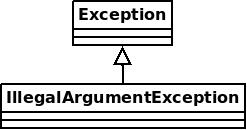
\includegraphics[scale=.4]{../img/oo-exception}
  \end{center}
  si on �crit \java|Exception| dans le \java|catch|
  \begin{itemize}
  \item on attrape \java|IllegalArgumentException|
  \item mais aussi d'autres exceptions  $\Longrightarrow$ � �viter
  \end{itemize}
\end{itemize}
\end{frame}


% === Cours de Java
% === Chapitre : Liste 

\section{Les listes}

\leconwithtoc

\subsection{ArrayList}

\begin{frame}{Pr�sentation}
En Logique, vous avez vu le concept de \textit{Liste}
\\\bigskip
\emph{Liste} : S�quence d'�l�ments (ordonn�s mais pas n�cessairement tri�s) auxquels on acc�de via leur \emph{position}
\\\bigskip
Ce concept est pr�sent en \sigle{Java}
\begin{itemize}
  \item Pas dans le langage
  \item Mais via l'API standard \\(classe \java|java.util.ArrayList|)
\end{itemize}
\end{frame}

\begin{frame}[fragile]{D�claration / Cr�ation}
\begin{Java}
  ArrayList<String> liste = new ArrayList<String> ();
\end{Java}
\medskip
\begin{itemize}
\item On sp�cifie le type des �l�ments (via les \java|<>|)
\item Cr�e une liste \emph{vide}
\item Elle pourra �videmment grandir au besoin \\(pas de limite)
\end{itemize}
\end{frame}

\begin{frame}[fragile]{D�claration / Cr�ation}
�criture viellie (\emph{non recommand�e}) : \\Ne pas mettre les \java|<>|
\begin{Java}
  ArrayList liste = new ArrayList ();
\end{Java}
\medskip

\includegraphics[scale=.5]{../img/java7.jpeg}En Java7, on peut ne pas sp�cifier le type des �l�ments � droite (d�duit par le compilateur)
\begin{Java}
  ArrayList<String> liste = new ArrayList<>();
\end{Java}
\end{frame}

\begin{frame}[fragile]{Ajout d'�l�ments}
\begin{tabular}{r|l}
  \java|add(E)|      & ajoute en fin \\
  \java|add(int, E)| & ajoute (ins�re) en position donn�e \\
\end{tabular}
\medskip
\begin{itemize}
\item Le premier �l�ment est en position \emph{0}
\item Une insertion provoque un d�calage des �l�ments suivants
\end{itemize}
\emph{Exemple} :
\begin{Java}
  ArrayList<String> dictionnaire = new ArrayList<String>(); 
  dictionnaire.add("z�bre");
  dictionnaire.add("�l�phant");
  dictionnaire.add(1, "girafe");
  // contient : [ "z�bre", "girafe", "�l�phant" ]
\end{Java}
\end{frame}

\begin{frame}[fragile]{Affichage}
La m�thode \java|toString| a �t� r�crite pour afficher les �l�ments
\\\bigskip
\emph{Exemple} :
\begin{Java}
  ArrayList<String> dictionnaire = new ArrayList<String>(); 
  dictionnaire.add("z�bre");
  dictionnaire.add("�l�phant");
  dictionnaire.add(1, "girafe");
  System.out.println( dictionnaire );
  // affiche : [ "z�bre", "girafe", "�l�phant" ]
\end{Java}
\end{frame}

\begin{frame}[fragile]{Taille de la liste}
\begin{tabular}{r|l}
  \java|size()|      & donne la taille \\
  \java|isEmpty()|   & indique si c'est vide \\
\end{tabular}
\bigskip
\\\emph{Exemple} :
\begin{Java}
  ArrayList<String> dictionnaire = new ArrayList<String>();
  System.out.println( dictionnaire.size() );    // 0
  System.out.println( dictionnaire.isEmpty() ); // true
 dictionnaire.add("z�bre");
 dictionnaire.add("�l�phant");
 dictionnaire.add(1, "girafe");
  System.out.println( dictionnaire.size() );    // 3
  System.out.println( dictionnaire.isEmpty() ); // false
\end{Java}
\end{frame}

\begin{frame}[fragile]{Acc�s aux �l�ments}
\begin{tabular}{r|l}
  \java|get(int)|    & demande un �l�ment \\
\end{tabular}
\bigskip
\begin{itemize}
\item Permet notamment le parcours
\end{itemize}
\emph{Exemple} :
\begin{Java}
public static void monAffichage( ArrayList<String> liste ) {
  for(int i=0; i<liste.size(); i++) {
     System.out.println( i + ": " + liste.get(i) );
  }
}
\end{Java}
\end{frame}

\begin{frame}[fragile]{Parcours}
Parcours d'une liste via le \emph{foreach} :
\\\bigskip
\emph{Exemple} :
\begin{Java}
  for (String mot : dictionnaire){ 
    System.out.println(mot);
  }
\end{Java}
\begin{itemize}
  \item La variable \texttt{mot} prend chaque valeur de la liste
  \item La position de \texttt{mot} est inconnue : remplacement/suppression
  impossibles
\end{itemize}
\end{frame}

\begin{frame}[fragile]{Remplacement}
\begin{tabular}{r|l}
  \java|set(int, E)| & remplace l'�l�ment en position donn�e \\
\end{tabular}
\\\bigskip
\emph{Exemple} :
\begin{Java}
public static void remplacer( ArrayList<String> dico ) {
  String mot ; 
  for (int i=0; i<dico.size(); i++ ) {
     mot = dico.get(i);
     if (mot.charAt(0) == 'a') {
        dico.set(i,"remplac�");
     }
  }
}
\end{Java}
\end{frame}

\begin{frame}{Recherche}
\begin{center}
\begin{tabular}{r|l}
  \java|boolean contains(E)| & indique si l'�l�ment est pr�sent  \\
  \java|int indexOf(E)|   & donne l'indice de la 1�re occurence \\
                          & de l'�l�ment dans la liste\\
\end{tabular}
\end{center}
\medskip 
Recherche un �l�ment de \emph{m�me valeur}
\begin{itemize}
\item Utilisation de la m�thode \java|equals|
\item N�cessit� de la red�finir pour nos propres classes
\end{itemize}
\end{frame}

\begin{frame}{Suppression}
\begin{center}
\begin{tabular}{r|l}
  \java|remove(int)| & enl�ve l'�l�ment en position donn�e \\
  \java|remove(E)|   & enl�ve un �l�ment donn� \\
\end{tabular}
\end{center}
\medskip 
\begin{itemize}
\item Comme pour la recherche, se base sur la m�thode \java|equals|
\item Pas de m�thode pour supprimer le dernier mais on peut �crire 
\java|liste.remove( liste.size()-1 )|
\end{itemize}
\end{frame}

\subsection{Wrapper}

\begin{frame}{Wrapper}
Seuls les objets sont permis dans les listes.
\begin{itemize}
\item Et pour les types primitifs (\java|int|, \java|boolean|, \dots) ?
\item Existence de \textit{wrapper} (\textit{enveloppe})
  \begin{itemize}
  \item Englobe une valeur primitive dans un objet
  \item Conversion automatique de l'un � l'autre
  \end{itemize}
\end{itemize}
\begin{center}
\begin{tabular}{r|l}
  Type primitif & Enveloppe \\\hline
  \java|int| & \java|Integer| \\
  \java|boolean| & \java|Boolean| \\
  \java|char| & \java|Character| \\
  \dots & \dots \\
\end{tabular}
\end{center}
\end{frame}

\begin{frame}[fragile]{Wrapper}
\emph{Exemple} : Combien de conversions automatiques en tout ?
\begin{Java}
import java.util.ArrayList ;
public class TestBox {
  public static void main ( String[] args ) {
    ArrayList<Integer>  liste = new ArrayList<Integer>() ;
    liste.add(1) ; liste.add(14); liste.add(1) ;
    int premier = liste.get(0);
    liste.set(2, liste.get(2) + 1 );
  }
}
\end{Java}
\end{frame}

\subsection{LinkedList}

\begin{frame}{LinkedList}
La classe \java|LinkedList| propose aussi le concept de \textit{Liste}
\begin{itemize}
\item On retrouve toutes les m�thodes vues pour \java|ArrayList|
\item Pouquoi plusieurs versions ?
  \begin{itemize}
  \item Font la m�me chose
  \item \emph{mais} diff�rences en terme de performances 
  \end{itemize}
\end{itemize}
\pause
\begin{small}
\begin{center}
\begin{tabular}{p{4cm}|p{6cm}}
  \java|ArrayList| & \java|LinkedList| \\
  \hline\hline
  �l�ments stock�s dans un tableau & �l�ments stock�s dans une liste chain�e (cf. Logique 2�me) \\
  \hline
  recommand� en g�n�ral & parfois plus rapide \\
  (ex: plus rapide pour acc�der � un �l�ment) & (ex: ajout en d�but)  \\
\end{tabular}
\end{center}
\end{small}
\end{frame}

\subsection{Interface}

\begin{frame}[fragile]{Le concept d'interface}
Supposons qu'on veuille �crire une m�thode qui affiche un �l�ment sur deux
  \begin{itemize}
  \item d'une \java|ArrayList| de chaines
  \begin{Java}
  public static void afficher1Sur2(ArrayList<String> liste) {
      for( int i=0; i<liste.size(); i+=2 ) {
          System.out.println( liste.get(i) );
      }
  } 
  \end{Java}
  \item d'une \java|LinkedList| de chaines
  \begin{Java}
  public static void afficher1Sur2(LinkedList<String> liste) {
      for( int i=0; i<liste.size(); i+=2 ) {
          System.out.println( liste.get(i) );
      }
  } 
  \end{Java}
  \end{itemize}
\end{frame}

\begin{frame}[fragile]{Le concept d'interface}
Le code �crit est presque identique
  \begin{itemize}
  \item Seule la d�claration du param�tre change
  \end{itemize}
\bigskip
On aimerait �viter de dupliquer le code
  \begin{itemize}
  \item Indiquer qu'on accepte une \java|ArrayList| \emph{ou} une \java|LinkedList|
  \item Et m�me n'importe quelle classe qui d�finit le concept de liste
  \item En fait, il nous suffit que les m�thodes d'une liste existent
  \end{itemize}
\end{frame}

\begin{frame}[fragile]{Interface}
\emph{Interface} : suite de d�clarations de m�thodes
\\\medskip\emph{Exemple} :
\begin{Java}
  interface MonInterface {
      void maM�thode1(int a);
      boolean maM�thode2(char c);
  } 
\end{Java}
\begin{itemize}
\item Notez les \java|;|
\item On donne l'ent�te mais pas le code
\end{itemize}
\end{frame}

\begin{frame}[fragile]{Interface}
\emph{Impl�menter une interface} : D�finir toutes les m�thodes d'une interface
\\\medskip\emph{Exemple} :
\begin{Java}
  public MaClasse implements MonInterface {
      public void maM�thode1(int a) {// le corps de la m�thode...}
      boolean maM�thode2(char c) {// le corps de la m�thode...}
      // + d'autres m�thodes si on veut
  } 
\end{Java}
\begin{itemize}
\item On d�clare qu'on impl�mente l'interface
\item Le compilateur v�rifie qu'on fournit bien le code de chaque m�thode
\end{itemize}
\end{frame}

\begin{frame}{Interface List}
Il existe une interface \java|List|
\begin{itemize}
\item D�finit toutes les m�thodes d�j� vues pour les listes
\item Impl�ment�e par \java|ArrayList| et \java|LinkedList|
\item Se voit facilement dans la \textit{javadoc}
\end{itemize}
\end{frame}

\begin{frame}[fragile]{Interface et polymorphisme}
Une interface d�finit un \textit{type}
\begin{itemize}
\item On peut donc utiliser une interface dans une d�claration (variable, param�tre, \dots)
\item L� o� une interface est attendue, on peut trouver n'importe quelle classe l'impl�mentant
(polymorphisme)
\end{itemize}
\emph{Exemple} : 
\begin{Java}
  public static void afficher1Sur2( List<String> liste ) {
    for (int i=0; i<liste.size(); i+=2) {
      System.out.println( liste.get(i) );
    }
  }
\end{Java}
\end{frame}

\begin{frame}[fragile]{Programmation par interface}
\emph{Bon usage} : programmer le plus possible avec les interfaces (et pas l'impl�mentation)
\begin{itemize}
  \item Choix de l'impl�mentation uniquement lors de l'instanciation
  \begin{Java}
  List<String> maListe;
  maListe = new ArrayList<String>();
  \end{Java}
  \item Assure que l'on ne va utiliser que les m�thodes d�finies dans l'interface
  \item Facilite le changement d'impl�mentation
\end{itemize}
\end{frame}

\subsection{Collections}

\begin{frame}{Collections}
La classe \java{java.util.Collections} propose des services pour les listes
\begin{center}
\begin{tabular}{r|l}
  \java|max ( List )| & donne le maximum d'une liste \\
  \java|sort ( List )| & trie une liste \\
  \java|reverse ( List )| & inverse une liste \\
  \java|shuffle ( List )| & m�lange une liste \\
  \dots & \dots \\
\end{tabular}
\end{center}
\end{frame}

\begin{frame}[fragile]{Collections}
\emph{Exemple} : 
\begin{Java}
   List<String> animaux = new ArrayList<String>() ;  

   animaux.add("�ne");
   animaux.add("z�bre");
   animaux.add("alouette");

   System.out.println (Collections.max(animaux) );
\end{Java}
affiche \textit{�ne} (pourquoi pas \textit{z�bre} ) ?
\end{frame}


\section{Les exceptions}
\leconwithtoc

\subsection{Pr�sentation}

\begin{frame}{Pr�sentation}
Parfois, le programme se trouve face � une 
\\\emph{situation anormale}
\bigskip
  \begin{itemize}
  \item Peut �tre d�tect�e par
    \begin{itemize}
    \item la \sigle{JVM} (ex: division par 0)
    \item ou le code \sigle{Java} (ex: param�tre invalide)
    \end{itemize}
  \item Une exception est cr��e par le code qui a d�tect� le probl�me
  \item L'exception est \emph{lanc�e}
  \item Un autre bout de code peut \emph{attraper} l'exception
    \begin{itemize}
    \item normalement pour r�soudre le probl�me
    \end{itemize}
  \end{itemize} 
\end{frame}

\begin{frame}[fragile]{Lancer une exception}
Quand une situation anormale est d�tect�e, il faut le signaler
  \begin{itemize}
  \item Cr�er un objet de type \java{Exception} (ou un fils)
  \item Le lancer
  \item La suite de la m�thode n'est pas ex�cut�e
  \end{itemize}
\bigskip\emph{Exemple}
\begin{Java}
void f(int nb) {
  if (nb<0)
       throw new IllegalArgumentException("Nombre n�gatif");
  // La suite normale...
}
\end{Java}
\end{frame}

\begin{frame}[fragile]{Itin�raire d'une exception}
Une exception remonte la <<pile d'appel>> jusqu'� ce qu'un bout de code d�di� l'attrape.
\\\bigskip
\emph{Exemple} : \java{main} appelle \java{f} qui appelle \java{g}       
\begin{itemize}
\item[]
  \begin{Java}
  void g() { int nb = Integer.parseInt("Douze"); }
  \end{Java}
\item \java{g} ne g�re pas l'exception, elle passe � \java{f}
\item Si \java{f} ne la g�re pas, elle passe � \java{main}
\item Si \java{main} ne la g�re pas, elle passe � la \sigle{JVM}
\item La \sigle{JVM} attrape tout, affiche un message complet et arr�te le programme
\end{itemize}
\end{frame}

\begin{frame}[fragile]{Attraper une exception}
Si on veut attraper une exception
\begin{itemize}
\item On englobe la partie qui peut poser probl�me par \java{try}
\item La partie \java{catch} contient la gestion de l'exception
\end{itemize}
\bigskip\emph{Exemple}
\begin{Java}
try {
      nb = Integer.parseInt(chaine);
} catch (NumberFormatException ex) {
      // gestion de l'exception
}
\end{Java}
  \begin{itemize}
  \item La m�thode \java|parseInt| (ou une m�thode appel�e par elle) contient un 
  \java|throw new NumberFormatException(...)|
  \end{itemize} 
\end{frame}

\begin{frame}[fragile]{R�sumons}
\vspace{-20pt}
D�roulement quand \emph{tout va bien}
\begin{columns}[T]
\begin{column}{0.12\textwidth}
\begin{Java}
main() {
  ...
  f()
  ...
}
  \end{Java}
\end{column}
\begin{column}{0.3\textwidth}
\begin{Java}[escapechar=\%]
f() {
  ...
  try {
    ...
    g()
    ...
  } catch(...) {
    %\emph{... // Pas fait !}%
  }
  ...
}
\end{Java}
\end{column}
\begin{column}{0.23\textwidth}
\begin{Java}
g() {
    ...
    h()
    ...
}
\end{Java}
\end{column}
\begin{column}{0.25\textwidth}
\begin{Java}
h() {
  ...
  if (test)
      throw... 
  ...
}
\end{Java}
\end{column}
\end{columns}
\medskip
Si le test est faux 
\\$\Longrightarrow$ le code du <<catch>> (en brun) n'est pas ex�cut�
\end{frame}

\begin{frame}[fragile]{R�sumons}
\vspace{-20pt}
D�roulement quand un \emph{probl�me} est d�tect�
\begin{columns}[T]
\begin{column}{0.12\textwidth}
\begin{Java}
main() {
  ...
  f()
  ...
}
  \end{Java}
\end{column}
\begin{column}{0.3\textwidth}
\begin{Java}[escapechar=\%]
f() {
  ...
  try {
    ...
    g()
    %\emph{... // Pas fait !}%
  } catch(...) {
    ... 
  }
  ...
}
\end{Java}
\end{column}
\begin{column}{0.23\textwidth}
\begin{Java}[escapechar=\%]
g() {
 ...
 h()
 %\emph{... // Pas fait !}%
}
\end{Java}
\end{column}
\begin{column}{0.25\textwidth}
\begin{Java}[escapechar=\%]
h() {
  ...
  if (test)
      throw... 
  %\emph{... // Pas fait !}%
}
\end{Java}
\end{column}
\end{columns}
\medskip
Si le test est vrai 
\\$\Longrightarrow$ les codes en brun ne sont pas ex�cut�s
\end{frame}

\begin{frame}[fragile]{Une exception est un objet}
\emph{Exemple}
\begin{Java}
  } catch (NumberFormatException ex) {
\end{Java}
  \begin{itemize}
  \item On sp�cifie qu'on attrape tout objet de la classe \java|NumberFormatException|
  \item Et qu'on va l'appeler \java|ex| dans le corps du \java|catch|
  \item On pourra poser des questions � cet objet 
    \begin{itemize}
    \item Pr�cisions sur le probl�me
    \item \emph{exemple} : \java|ex.getMessage()|
    \end{itemize}
  \end{itemize}
\end{frame}

\begin{frame}[fragile]{Hi�rarchie des exceptions}
Cette hi�rarchie des exceptions explique pourquoi on peut �crire :
  \begin{itemize}
  \item[]
    \begin{Java}
    } catch (Exception ex) {
    \end{Java}
  \item \java{NumberFormatException} h�rite de \java{Exception}
  \item Mise en oeuvre du polymorphisme
  \end{itemize}
\bigskip
\warning{� �viter car on attrape aussi d'\emph{autres} exceptions. (qu'on ne saura peut-�tre pas traiter)}
\end{frame}

\begin{frame}[fragile]{Attraper plusieurs exceptions}
On peut attraper plusieurs types d'exceptions
\\\bigskip\emph{Exemple}
\begin{Java}
try {
      nb = Integer.parseInt(chaine);
} catch (NumberFormatException ex) {
      // La chaine ne contient pas un int
} catch (Exception ex) {
      // Autre probl�me
}
\end{Java}
  \begin{itemize}
  \item On ex�cute le premier \java{catch} qui est en ad�quation avec l'exception
lanc�e
  \end{itemize}
\end{frame}

\begin{frame}[fragile]{Attraper plusieurs exceptions}
L'ordre � son importance
\\\bigskip\emph{Exemple}
\begin{Java}
try {
      nb = Integer.parseInt(chaine);
} catch (Exception ex) {
      // Autre probl�me
} catch (NumberFormatException ex) {
      // La chaine ne contient pas un int
}
\end{Java}
  \begin{itemize}
  \item En cas de \java{NumberFormatException} c'est la partie \java{Exception} 
        qui est activ�e
        \\ $\Rightarrow$ Interdit par le compilateur
  \end{itemize}
\end{frame}

\begin{frame}[fragile]{Exemple complet}
\begin{Java}
public class Outil 
{
  public static void afficherLigne(int nb) {
    if (nb<1 || nb >80)
        throw new IllegalArgumentException("taille entre 1 et 80 !");
    for( int i=1; i<=nb; i++) {
        System.out.print('-');
    }
    System.out.println();
  }

  public static void usage() {
    System.out.println("usage: java Test nb (1 � 80)");
    System.exit(1);
  }
}
\end{Java}
\end{frame}

\begin{frame}[fragile]{Exemple complet}
\begin{Java}
public class Test 
{
  public static void main(String[] args) {
    int nb = 0;
    if (args.length != 1) Outil.usage();
    try {
        nb = Integer.parseInt(args[0]);
    } catch (NumberFormatException ex) {
        Outil.usage();
    }
    try {
        Outil.afficherLigne( nb );
    } catch (IllegalArgumentException ex) {
        Outil.usage();
    }
  }
}
\end{Java}
\end{frame}

\begin{frame}[fragile]{Exemple complet}
Ou bien (code moins �clat�)
\begin{Java}
public class Test 
{
  public static void main(String[] args) {
    if (args.length != 1) Outil.usage();
    try {
        int nb = Integer.parseInt(args[0]);
        Outil.afficherLigne( nb );
    } catch (NumberFormatException ex) {
        Outil.usage();
    } catch (IllegalArgumentException ex) {
        Outil.usage();
    }
  }
}
\end{Java}
\end{frame}

\begin{frame}[fragile]{Exemple complet}
Ou encore (dangereux : on capture toutes les erreurs)
\begin{Java}
public class Test 
{
  public static void main(String[] args) {
    if (args.length != 1) Outil.usage();
    try {
        int nb = Integer.parseInt(args[0]);
        Outil.afficherLigne( nb );
    } catch (Exception ex) {
        Outil.usage();
    }
  }
}
\end{Java}
\end{frame}


\begin{frame}[fragile]{Exemple complet}

\includegraphics[scale=.5]{../img/java7.jpeg}En Java 7, on peut combiner des exceptions 
\begin{Java}
public class Test 
{
  public static void main(String[] args) {
    if (args.length != 1) Outil.usage();
    try {
        int nb = Integer.parseInt(args[0]);
        Outil.afficherLigne( nb );
    } catch (NumberFormatException | IllegalArgumentException ex) {
        Outil.usage();
    }
  }
}
\end{Java}
\end{frame}

\subsection{Exceptions contr�l�es}

\begin{frame}[fragile]{Exceptions contr�l�es}
Philosophie de \sigle{Java} : obliger le programmeur � coder proprement
\begin{itemize}
\item $\Rightarrow$ Toute exception devrait �tre g�r�e
\item Mais beaucoup d'instructions peuvent provoquer une exception 
(ex: \java{ArrayIndexOutOfBoundsException})
\item On ne peut pas mettre des \java{try} partout
\item $\Rightarrow$ Java diff�rencie les exceptions
\end{itemize}
\end{frame}

\begin{frame}[fragile]{Diff�rentes sortes d'exceptions}
\begin{center}
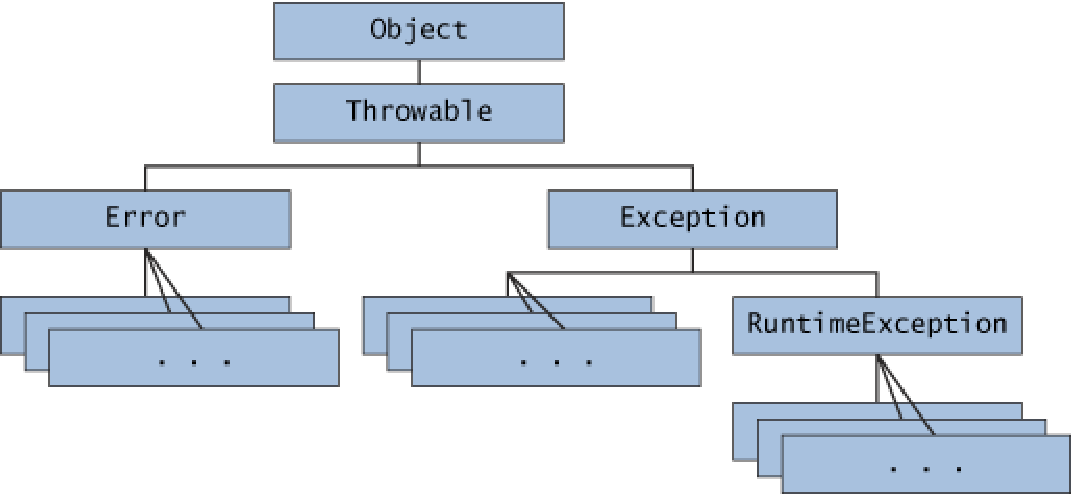
\includegraphics[scale=.5]{../img/exceptions-throwable} 
\\
\begin{tiny}
source: \code|http://java.sun.com/docs/books/tutorial/essential/exceptions/index.html|
\end{tiny}
\end{center}
\java|java.lang.Throwable| : type commun � toutes les exceptions
\end{frame}

\begin{frame}[fragile]{Diff�rentes sortes d'exceptions}
\java|Exception|
  \begin{itemize}
  \item Toutes les exceptions \emph{contr�l�es} par le compilateur
  \item On doit \emph{explicitement} les g�rer ou les laisser passer. Sauf pour\dots
  \end{itemize} 
\bigskip
\java|RuntimeException|
  \begin{itemize}
  \item Sous-ensemble de \code{Exception}
  \item Pas d'obligation de les traiter
  \end{itemize} 
\bigskip
\java|Error| 
  \begin{itemize}
  \item Li�es au dysfonctionnement de la machine virtuelle
  \item Il est d�conseill� de les traiter
  \end{itemize} 
\end{frame}

\begin{frame}[fragile]{Exceptions contr�l�es}
Si une m�thode \emph{peut} lancer une exception \emph{contr�l�e}
\begin{itemize}
  \item Elle doit le d�clarer dans la signature
  \begin{Java}
void f() throws IOException {
  ...
  if (...)
    throw new IOException("...");
  ...
}
  \end{Java}
  \item \emph{Remarque} : ne pas confondre \java{throw} et \java{throws}
\end{itemize}
\end{frame}

\begin{frame}[fragile,allowframebreaks]{Exceptions contr�l�es}
Quand on appelle une m�thode qui \emph{peut} lancer une exception \emph{contr�l�e}
  \begin{itemize}
  \item On est \emph{oblig�} de la g�rer
\begin{Java}
void g() {
  ...
  try {
    f();
  } catch( IOException ex ) {
    // g�rer l'exception
  }
  ...
}
\end{Java}
\item \emph{ou} de d�clarer qu'on la lance 
 \\(qu'on la laisse passer en fait)
\begin{Java}
void g() throws IOException {
  ...
  f();
  ...
}
\end{Java}
\item Tout cela est v�rifi� par le compilateur
\end{itemize}
\end{frame}

\subsection{Cr�er ses exceptions}

\begin{frame}[fragile]{Cr�er ses propres exceptions}
Revient � cr�er une classe qui h�rite de \java{Exception} \\(ou \code|RuntimeException|)
\smallskip
\\\emph{Exemple} :
\begin{Java}
public class NombreN�gatifException extends Exception {
    public NombreN�gatifException(String s) {
        super(s);
    }
}
\end{Java}
\begin{itemize}
\item \java|extends Exception| indique que la classe h�rite de \java|Exception|
\item \java|super(s)| est li� � l'h�ritage.\\On appelle le constructeur du parent
\end{itemize}
\end{frame}

\begin{frame}[fragile]{Cr�er ses propres exceptions}
\emph{Exemple} : Lancer et capturer une exception propre
\begin{Java}
public class Test {
    public void afficherLignes(int nb) throws NombreN�gatifException {
        if (nb<0)
            throw new NombreN�gatifException("�a coince");
        // la suite normale...
    }

    public static void main(String[] args) {
        Test test = new Test();
        try {
            test.afficherLignes(args[0]);
        } catch (NombreN�gatifException ex) {
            System.out.println(ex.getMessage());
        }
    }
}
\end{Java}
\end{frame}

\begin{frame}[fragile]{Exemple complet}
\begin{Java}[basicstyle=\scriptsize]
public class Groupe {    

    private Etudiant[] �tudiants;
    private int nbEtudiants;

    public Groupe(int tailleGroupe) {
        �tudiants = new Etudiant[tailleGroupe];
        nbEtudiants = 0;
    }
    
    public void ajouter(Etudiant �tudiant) 
                                 throws D�passementCapacit�Exception {
        if (nbEtudiants == �tudiants.length)
            throw new D�passementCapacit�Exception("Plus de place !");

        �tudiants[nbEtudiants] = �tudiant;
        nbEtudiants++;
    }

    // Les autres m�thodes ici    
}
\end{Java}
\end{frame}

\begin{frame}[fragile]{Exemple complet}
\begin{Java}
public class D�passementCapacit�Exception extends Exception {
    public D�passementCapacit�Exception(String s) {
        super(s);
    }    
}
\end{Java}
\bigskip
\emph{Remarque} : Si on n'avait pas fait le test de d�passement de capacit�
  \begin{itemize}
  \item \java|ajouter| aurait lanc� une \java|IndexOutOfBoundsException|
  \item Pas clair pour l'utilisateur (qui n'a pas connaissance de l'impl�mentation)
  \end{itemize}
\end{frame}

\begin{frame}[fragile]{La clause <<finally>>}
\begin{itemize}
\item La clause \java{finally} est toujours ex�cut�e
\item � la fin du \java{try} ou apr�s le \java{catch}
  \begin{itemize}
  \item M�me en pr�sence d'un \java|return|
  \item ou si une exception est lanc�e dans le \java|catch|
  \end{itemize}
\item Permet d'indiquer un code qui doit toujours �tre ex�cut�
\item Rarement utilis� (par ex: pour fermer une ressource externe comme un fichier)
\end{itemize}
\end{frame}

\begin{frame}[fragile]{Le try avec ressource}

\includegraphics[scale=.5]{../img/java7.jpeg} Java 7
\begin{itemize}
\item Permet de s'assurer qu'une ressource sera bien lib�r�e
\\(un fichier par exemple)
\item Plus facile et plus s�r que via la clause \java|finally|
\item Plus d'info dans la le�on sur les entr�es-sorties
\item \emph{Exemple}
\begin{Java}
    try (InputStream fis = new FileInputStream(source)) {
        // traitement du fichier
    }   // ...
\end{Java}
\end{itemize}
\end{frame}

%\begin{frame}[fragile]{La clause <<finaly>>}
%\emph{Exemple}
%\begin{Java}
%public class A {
%    public static void foo() {
%        B b = new B();
%        try {
%            b.leveException();
%        } catch (MyException e) {
%            System.out.println("hum! some problems");
%        } finally {
%            System.out.println("fin de foo");
%        }
%    }
%}
%\end{Java}
%\end{frame}

%\begin{frame}[fragile]{Utiliser judicieusement les exceptions}
%Cas le plus fr�quent d'utilisation : v�rifier les param�tres
%\begin{Java}
%void f(...) {
%  if (...)
%    throw new IllegalArgumentException("...");
%}
%\end{Java}
%\bigskip
%\warning{N'attraper une exception qui si on est \emph{capable} de la traiter.
%Sinon, la laisser passer.}
%\end{frame}


\section{Les entr�es-sorties (IO)}
\leconwithtoc

\subsection{Pr�sentation}

\begin{frame}{Pr�sentation}
Rappel : En \sigle{Logique} vous avez vu
  \begin{itemize}
  \item Les fichiers \emph{s�quentiels} \emph{structur�s}
  \item En \emph{entr�e} ou en \emph{sortie} (mais pas les 2)
  \end{itemize}
\bigskip
Possible aussi en \sigle{Java} (et bien plus)
\begin{itemize}
  \item Mais plus complexe
  \item On doit s'int�resser aux aspects pratiques
    \begin{itemize}
    \item Comment coder l'information \\(texte, binaire, s�rialisation, \dots)  
    \item Comment g�rer les erreurs (fichier inexistant, \dots)
    \end{itemize}
  \end{itemize}
\end{frame}

\begin{frame}{Coder l'information}
En \sigle{java}, on peut coder l'information de 2 fa�ons
  \begin{description}
  \item[Binaire] : On utilise la repr�sentation m�moire
  \item[Texte] : On utilise une suite de caract�res
  \end{description}
\bigskip\emph{Exercice} : Soit l'entier $16$
    \begin{itemize}
    \item Donner les repr�sentations <<binaire>> et <<texte>>
    \item Quelles sont les tailles de ces repr�sentations ? 
    \item Voyez-vous des avantages/inconv�nients � ces repr�sentations ?
    \end{itemize}
\end{frame}

\begin{frame}{Types de fichiers}
En \sigle{java}, les fichiers sont \emph{uniformes}
  \begin{description}
  \item[Fichier binaire] : Tout est cod� en binaire
  \item[Fichier texte] : Tout est cod� en caract�res
  \end{description}
\bigskip
Ce n'est pas indiqu� dans le fichier
    \begin{itemize}
    \item Il faut le savoir et utiliser le fichier en cons�quence
    \item Sinon le r�sultat n'est pas celui esp�r�
    \end{itemize}
\bigskip\emph{Exercice} : Si on cr�e un fichier binaire avec l'entier 16 et qu'on le relit comme un fichier texte que se passe-t-il ?
\end{frame}

\begin{frame}{Types de fichiers}
Par contre les fichiers ne sont \emph{pas structur�s}
    \begin{itemize}
    \item On peut m�langer le contenu
    \item \emph{Ex} : �crire un entier puis une chaine puis un r�el
    \end{itemize}
\bigskip
On ne peut pas demander ce qui s'y trouve, il faut le savoir.
\end{frame}

\begin{frame}{Vue d'ensemble}
Au niveau le plus bas, \sigle{Java} fournit des classes et m�thodes pour lire/�crire
  \begin{itemize}
  \item des \java|byte| dans un fichier \emph{binaire}
  \item des \java|char| dans un fichier \emph{texte}
  \end{itemize}
\bigskip
D'autres classes sp�cialis�es vont permettre de lire/�crire
  \begin{itemize}
  \item Des valeurs primitives
  \item Des objets (via la <<s�rialisation>>)
  \end{itemize}
\bigskip
Presque tout se trouve dans le package \java|java.io|
\end{frame}

% Ce n'est, a mon sens pas la meilleure image, mais je n'en ai pas d'autres
% --pbt
\begin{frame}{Vue d'ensemble}
\begin{center}
\includegraphics[scale=.45]{../img/java-io-schema}
\end{center}
\end{frame}

\subsection{Fichier binaire}
\leconwithtocinside

\begin{frame}[fragile]{Lecture dans un fichier binaire}
\emph{Exemple} : Lire le contenu d'un fichier binaire 
\begin{Java}
int b;
try {
    FileInputStream in = new FileInputStream("nomFichier");
    b = in.read();    
    while( b != -1 ) {
        System.out.print(b+" ");
        b = in.read();    
    }
    in.close();   
} catch ( IOException ex ) {
    // g�rer le probl�me ici si possible
}
\end{Java}
\end{frame}

\begin{frame}[fragile]{Lecture dans un fichier binaire}
\emph{D�claration du fichier}
  \begin{itemize}
  \item \java|FileInputStream| permet la lecture dans un fichier binaire
  \item On ne sp�cifie pas le contenu (non structur�)
  \end{itemize}
\medskip
\emph{Ouverture}
  \begin{itemize}
  \item Se fait lors de l'instanciation de la classe
  \item C'est ici qu'on fait le lien avec le fichier physique
  \end{itemize}
\end{frame}

\begin{frame}[fragile]{Lecture dans un fichier binaire}
\emph{Fermeture}
  \begin{itemize}
  \item Via la m�thode \java|close|
  \end{itemize}
\bigskip
\emph{Lecture dans le fichier}
  \begin{itemize}
  \item Via la m�thode \java|read|
  \end{itemize}
\bigskip
\emph{Fin de fichier}
  \begin{itemize}
  \item La lecture de la valeur $-1$ indique la fin du fichier
  \end{itemize}
\bigskip
\emph{Remarque} La m�thode de lecture retourne un \java|int| et pas un \java|byte| 
\end{frame}

\begin{frame}[fragile]{Lecture dans un fichier binaire}
\emph{Exercice} : \textit{(compr�hension du concept de fichier binaire)}
\\Cr�ez un fichier qui contient
\begin{Java}
16

\end{Java}
et lisez-le avec le code pr�c�dent. 
\\Comprenez-vous le r�sultat ?
\end{frame}

\begin{frame}[fragile]{Lecture dans un fichier binaire}
\emph{Gestion des erreurs}
  \begin{itemize}
  \item L'exception li�e aux fichiers est \java|IOException|
  \item Pour l'ouverture en lecture il y a aussi \java|FileNotFoundException| 
  (qui h�rite de \java|IOException|)
  \item Elles sont contr�l�es par le compilateur \\(on doit en tenir compte)
  \end{itemize}
\end{frame}

\begin{frame}[fragile]{Lecture dans un fichier binaire}
On rencontre souvent une version compacte de la boucle de lecture
\begin{Java}
    int b;
    while ((b=file.read())!=-1) {
         System.out.print(b+" ");
    }
\end{Java}
  \begin{itemize}
  \item �vite la duplication du code de lecture
  \item Quid de la lisibilit� ?
  \end{itemize}
\end{frame}

\begin{frame}[fragile]{�criture dans un fichier binaire}
Pour l'�criture on utilise la classe \java|FileOutputStream|
\\\bigskip\emph{Exemple}
\begin{Java}
try {
    FileOutputStream out = new FileOutputStream("nomFichier");
    out.write(64);
    out.close();   
} catch ( IOException ex ) {
    // g�rer le probl�me ici si possible
}
\end{Java}
\bigskip
\emph{Exercice} : Afficher le contenu du fichier et comprendre le r�sultat.
\end{frame}

\begin{frame}[fragile]{�criture dans un fichier binaire}
\emph{Exemple} : copie d'un fichier
\begin{Java}
public static void copier( String nomIn, String nomOut )
                                             throws IOException {
    FileInputStream in = new FileInputStream(nomIn);
    FileOutputStream out = new FileOutputStream(nomOut);
    int b;
    while((b = in.read()) != -1) {
        out.write(b);
    }
    in.close();   
    out.close();
}
\end{Java}
  \begin{itemize}
  \item Appel possible : \java|copier("date.txt","data.bak");|
  \end{itemize}
\end{frame}

\begin{frame}[fragile]{�criture dans un fichier binaire}
\emph{Remarques}
\begin{itemize}
\item Cr�ation du fichier lors de l'instanciation
\item Si le fichier existe, son contenu est remplac�
\item Seul l'octet de poids faible est �crit \\(pourquoi accepter un \java|int| ?)
\item Pas de \java{FileNotFoundException}
\end{itemize}
\end{frame}

\begin{frame}[fragile]{�criture dans un fichier binaire}
\emph{Exemple} : autre possibilit� pour la copie
\begin{Java}
public static void copier( FileInputStream in, FileOutputStream out)
                                             throws IOException {
    int b;
    while((b = in.read()) != -1) {
        out.write(b);
    }
    in.close();   
    out.close();
}
\end{Java}
  \begin{itemize}
  \item Appel possible : 
  \begin{Java}
      copier( new FileInputStream("date.txt"),
              new FileOutputStream("data.bak") ); 
  \end{Java}
  \end{itemize}
\end{frame}

\subsection{Fichier texte}
\leconwithtocinside

\begin{frame}{Les fichiers textes}
M�mes principes que pour les fichiers binaires mais avec des classes adapt�es
\medskip
\begin{itemize}
\item \java|FileReader| pour lire un fichier texte
  \begin{itemize}
  \item \java|int read()| lit un caract�re (-1 si fin de fichier)
  \end{itemize}
\medskip
\item \java|FileWriter| pour �crire un fichier texte
  \begin{itemize}
  \item \java|void write(int c)| �crit le caract�re c
  \\(Seuls les 2 octets de poids faible sont �crits)
  \end{itemize}
\end{itemize}
\end{frame}

\begin{frame}[fragile]{Les fichiers textes}
\emph{Exemple} : lire le contenu d'un fichier texte
\begin{Java}
public static void cat( String nameIn) throws IOException {
    FileReader in = new FileReader(nameIn);
    int c;
    while((c = in.read()) != -1) {
        System.out.print(c);
    }



    in.close();   
}
\end{Java}
\emph{Exercice} : Corriger l'exemple pr�c�dent pour qu'il affiche fid�lement le contenu du fichier.
\end{frame}

\begin{frame}[fragile]{Les fichiers textes}
\emph{Exemple} : copie d'un fichier texte
\begin{Java}
public static void copier( String nameIn, String nameOut) 
                                          throws IOException {
    FileReader in = new FileReader(nameIn);
    FileWriter out = new FileWriter(nameOut);
    int c;
    while((c = in.read()) != -1) {
        out.write(c);
    }
    in.close();   
    out.close();
}
\end{Java}
\end{frame}


\subsection{Entr�es sorties buff�ris�es}
\leconwithtocinside 

\begin{frame}[fragile]{Entr�es sorties buff�ris�es}
Dans les exemples  vus, les lectures / �critures sont directement prises en
charge par l'OS
	\begin{itemize}
	\item risque d'entrainer des lenteurs
	\item Java propose de \emph{buff�riser} ses flux (\textit{buffered stream})
		\begin{itemize}
		\item le \textit{stream} lit dans un \textit{buffer}, lorsque le \textit{buffer} est
		vide l'API native est appel�e pour une lecture remplissant le buffer
		\item fonctionnement identique pour une �criture
		\end{itemize}
	\item ce type de flux est appel� \emph{flux englobant} 
	\end{itemize}
\end{frame}

\begin{frame}[fragile]{Entr�es sorties buff�ris�es}
Il existe 4 \textit{buffered stream}; 
\java|BufferedInputStream|, 
\java|BufferedOutputStream|, 
\java|BufferedReader| et 
\java|BufferedWriter|. 
\bigskip
On pourrait, par exemple, �crire 
\begin{Java}
BufferedReader inputStream = new BufferedReader(
    new FileReader("input.txt"));

BufferedWriter outputStream = new BufferedWriter(
    new FileWriter("output.txt"));
\end{Java}
\bigskip
\emph{Remarque} On force la vidange du flux via \java|flush|
\end{frame}



\subsection{Donn�es primitives}
\leconwithtocinside

\begin{frame}[fragile]{Donn�es primitives}
Concerne
  \begin{itemize}
  \item Tous les types primitifs
  \item Le type \java|String|
  \end{itemize}
\bigskip
Deux approches diff�rentes en fonction du format utilis�
  \begin{itemize}
  \item Fichier binaire
  \item Fichier texte
  \end{itemize}
\end{frame}

\begin{frame}[fragile]{Donn�es primitives sur un fichier binaire}
Pour �crire des donn�es primitives sur un fichier binaire on se base sur la classe \java|DataOutputStream|
\\\bigskip
\emph{Exemple}
\begin{Java}
try {
    DataOutputStream out = new DataOutputStream( 
                                   new FileOutputStream("nomFichier"));
    out.writeInt(16);
    out.writeUTF("Hello");    
    out.close();   
} catch ( IOException ex ) {
    // g�rer le probl�me ici si possible
}
\end{Java}
  \begin{itemize}
  \item La constructeur met bien en �vidence que �a se base sur un fichier binaire
  \end{itemize}
\end{frame}

\begin{frame}[fragile]{Donn�es primitives sur un fichier binaire}
Pour la lecture on se base sur la classe \java|DataInputStream|
\\\medskip
\emph{Exemple}
\begin{itemize}
\item[]
\begin{Java}
try {
    DataInputStream in = new DataInputStream( 
                                new FileInputStream("nomFichier"));
    int nb = in.readInt();
    String titre = in.readUTF();    
    in.close();   
} catch ( IOException ex ) {
    // g�rer le probl�me ici si possible
}
\end{Java}
\end{itemize}
\medskip
Pas de valeur sentinelle; g�n�re une \java|EOFException| si tentative de lecture au-del� de la fin du fichier.
\end{frame}

\begin{frame}[fragile]{Donn�es primitives sur un fichier binaire}
\emph{Exemple} : somme des nombres d'un fichier
\begin{Java}
  public double somme( DataInputStream in ) throws IOException {
      double somme = 0;
      try {
          while(true) {
              somme += in.readDouble();
          }
      } catch (EOFException ex) }
          // rien � faire, on passe simplement � la suite
      }
      return somme; 
  }
\end{Java}
\end{frame}

\begin{frame}[fragile]{Donn�es primitives sur un fichier texte}
Commen�ons par l'�criture sur fichier texte
\\\bigskip \emph{Exemple}
\begin{Java}
PrintWriter out = new PrintWriter(new FileOutputStream("result.dat"));
out.println(10);
out.print("Hello");
out.close();
\end{Java}
\bigskip \emph{Remarques}
\begin{itemize}
\item \java|PrintWriter| se base sur \java|FileOutputStream|
\item \java|print| et \java|println| fonctionnent comme vous les connaissez
\end{itemize}
\end{frame}

\begin{frame}[fragile]{Donn�es primitives sur un fichier texte}
On a d�j� abord� la classe \java|Scanner|
    \begin{itemize}
    \item Permet de lire au clavier (l'entr�e standard) 
    \item Offre des m�thodes de lecture : \java{nextInt()}, \dots
    \item Et aussi des m�thodes de test : \java|hasNextInt()|, \dots
    \item \emph{Exemple} 
	\begin{Java}
  import java.util.Scanner ; 
  ...
  Scanner clavier = new Scanner(System.in);
  int somme=0, nb;
  while (clavier.hasNextInt()) {
      somme += clavier.nextInt();
  } 
  System.out.println( somme );
	\end{Java}
\end{itemize}	
\end{frame}

\begin{frame}[fragile]{Donn�es primitives sur un fichier texte}
La classe \java|Scanner| fonctionne aussi avec un fichier texte
\\\bigskip\emph{Exemple} 
	\begin{Java}
  import java.util.Scanner ; 
  ...
  Scanner fileIn = new Scanner( new FileReader( "mesData" ) );
  int somme=0, nb;
  while (fileIn.hasNextInt()) {
      somme += fileIn.nextInt();
  } 
  System.out.println( somme );
	\end{Java}
\end{frame}

\subsection{Les <<flux>> standards}
\leconwithtocinside

\begin{frame}{La notion de <<flux>>}
Quelques points �tranges ne vous auront peut-�tre pas �chapp�s
  \begin{itemize}
  \item \java|Scanner| sert aussi bien pour un fichier que pour le <<clavier>>
  \item La m�thode \java|println| existe pour les fichiers mais aussi pour l'<<�cran>>
  \end{itemize}
\bigskip
En fait, le package \java|java.io| ne fonctionne pas uniquement avec des fichiers mais avec n'importe quel <<flux>> (<<stream>> en anglais)
\end{frame}

\begin{frame}{La notion de <<flux>>}
\emph{Flux} : �l�ment qui peut fournir ou recevoir une suite d'octets ou de caract�res
  \begin{itemize}
  \item Un \emph{clavier} peut �tre vu comme un flux fournissant des octets
  \item Un \emph{�cran} peut �tre vu comme un flux recevant des caract�res
  \item Et il y en a d'autres
    \begin{itemize}
    \item Un <<\emph{socket}>> (connection entre 2 ordinateurs)
    \item Une \emph{chaine} (fournit des caract�res)
    \item \dots
    \end{itemize}
  \end{itemize}
\end{frame}

\begin{frame}{La notion de <<flux>>}
\includegraphics[scale=.45]{../img/java-io-ins}
\begin{flushright}
\includegraphics[scale=.45]{../img/java-io-ins2} 
\end{flushright}
\begin{center}
{\scriptsize Source Oracle}
\end{center}
\end{frame}

\begin{frame}{Les flux standards}
Lorsqu'un programme s'ex�cute, 3 flux existent automatiquement
  \begin{itemize}
  \item � priori connect�s au clavier et � l'�cran
  \item Mais peut �tre chang� via une <<redirection>>
  \\(cf. cours de syst�me et exercices Linux au laboratoire)
  \end{itemize}
\bigskip
\java|System.in| : l'entr�e standard
  \begin{itemize}
  \item De type \java|InputStream|
    \begin{itemize}
    \item Classe g�n�rale pour un flux binaire en entr�e
    \item \java|FileInputStream| h�rite de \java|InputStream|
    \end{itemize}
  \end{itemize}
\end{frame}

\begin{frame}{Les flux standards}
\java|System.out| : la sortie standard
  \begin{itemize}
  \item De type \java|PrintStream|
  \item Ce qui explique l'existence de \java|println|
  \end{itemize}
\bigskip
\java|System.err| : l'erreur standard
  \begin{itemize}
  \item Aussi de type \java|PrintStream|
  \item Flux s�par� ce qui permet de ne rediriger que les erreurs
  \end{itemize}
\bigskip
\emph{Exercice} : Expliquez la nature de chacun des �l�ments de 
\java|System.out.println("Hello");|
\end{frame}

\subsection{Donn�es primitives formatt�es}
\leconwithtocinside

\begin{frame}[fragile]{Donn�es primitives formatt�es}
Les textes ayant pour vocation d'�tre lus par des humains
  \begin{itemize}
  \item On veut un \emph{contr�le fin} sur la \emph{mise en page} des textes produits
  \item On doit �tre capable de \emph{g�rer} une \emph{mise en page complexe} du texte lu
  \end{itemize}
\end{frame}

\begin{frame}[fragile]{�criture de donn�es formatt�es}
\java|PrintWriter| offre �galement la m�thode \java|printf| 
  \begin{itemize}
  \item Permet un contr�le tr�s fin de la sortie
  \item \emph{Exemple}
    \begin{Java}
public void test(PrintStream out) {  // Un fichier, l'�cran, ...
  out.printf("%04d\n", 23);	                     // 0023
  out.printf("%4.2f\n", 12.2);	                  // 12.20

  Calendar c = GregorianCalendar.getInstance();
  c.set(9, 00, 23);                              // 23 janvier 2009
  out.printf("le %1$td/%1$tm/%1$ty\n", c);       // le 23/01/09
}
    \end{Java}
  \item cf. l'API pour tous les d�tails
\end{itemize}
\end{frame}

\begin{frame}[fragile]{Lecture de donn�es formatt�es}
Voyons � pr�sent toute la puissance de \java|Scanner|
  \begin{itemize}
  \item Seule classe vue ici qui n'est pas dans \java|java.io|
  \item Permet de d�composer une suite de caract�res
  \item Fonctionne sur
    \begin{itemize}
    \item Un \java|InputStream| (fichier binaire, entr�e standard, \dots)
    \item Mais aussi un \java|String|
    \\\emph{Exemple} : \java|new Scanner("3 14 15 92 65")|
    \end{itemize}
  \item L'entr�e est d�compos�e en \emph{tokens}
    \begin{itemize}
    \item Cf. le�on sur l'analyse lexicale 
    \item Le s�parateur est le \emph{whitespace} (configurable)
    \end{itemize}
  \end{itemize}
\end{frame}

\begin{frame}[fragile]{Lecture de donn�es formatt�es}
Fonctionnement de base
  \begin{itemize}
  \item � la cr�ation on est au d�but
  \item Chaque \java|next()| \emph{lit} un token
  \item \java{nextType} �quivaut � un \java|next| suivi d'une conversion en le bon 
       \textit{type} (pour certains types)
  \item \emph{Exemple}
     \begin{Java}
  Scanner uneEntr�e = new Scanner("12 true \n false");
  // \n est un whitespace aussi !
  int n = uneEntr�e.nextInt();
  boolean b = uneEntr�e.nextBoolean();
  String s = uneEntr�e.next();
    \end{Java}  
  \end{itemize}
\end{frame}

\begin{frame}[fragile]{Lecture de donn�es formatt�es}
Si l'entr�e ne correspond pas au type demand� :
  \begin{itemize}
  \item \java|InputMismatchException| est lanc�e
  \item Le token n'est pas \emph{consomm�}
  \item \emph{Exemple}
    \begin{Java}
  Scanner uneEntr�e = new Scanner("true 12");
  int n = 0;
  try {
    n = uneEntr�e.nextInt();
  } catch (InputMismatchException ex) {
    uneEntr�e.next(); // N�cessaire !
    n = uneEntr�e.nextInt(); 
  }
    \end{Java}
  \end{itemize}
\end{frame}

\begin{frame}[fragile]{Lecture de donn�es formatt�es}
\java|nextLine()| lit la chaine jusqu'� la fin de la ligne (lue mais non incluse)
  \begin{itemize}
  \item \emph{Exemple}
    \begin{Java}
  Scanner uneEntr�e = new Scanner("12 true \n false");
  String s = uneEntr�e.nextLine(); //"12 true "
    \end{Java}
  \item \emph{Exemple}
    \begin{Java}
  Scanner uneEntr�e = new Scanner("12\n suite");
  int n = uneEntr�e.nextInt();
  String s = uneEntr�e.nextLine(); // lit "" !!!
  s = uneEntr�e.nextLine(); // lit " suite" !!!
    \end{Java}
  \end{itemize}
\end{frame}

\begin{frame}[fragile]{Lecture de donn�es formatt�es}
Pas de \java|nextChar()|
  \begin{itemize}
  \item Peut �tre simul� par \java|next().charAt(0)|
  \item \emph{Exemple}
    \begin{Java}
  Scanner uneEntr�e = new Scanner("12 suite");
  char c1 = uneEntr�e.next().charAt(0); // 1
  char c2 = uneEntr�e.next().charAt(0); // s
    \end{Java}
  \end{itemize}
\end{frame}

\begin{frame}[fragile]{Lecture de donn�es formatt�es}
On peut imposer un \emph{sch�ma} de lecture
  \begin{itemize}
  \item via \java|next(String pattern)|
  \item La syntaxe est tr�s riche et un peu complexe (cf. les expressions
r�guli�res (\textit{regex}), classe Pattern dans la documentation). 
  \item \emph{Exemple} : le token doit �tre le caract�re "H", "h", "F" ou "f" sinon 
     \java|InputMismatchException|
    \begin{Java}
  String s = clavier.next("[HhFf]");
    \end{Java}
  \end{itemize}
\end{frame}

\begin{frame}[fragile]{Lecture de donn�es formatt�es}
\begin{itemize}
	\item \emph{Exemple} : lire un op�rateur : +, -, * ou /
	\begin{Java}
  String s = clavier.next("[\\+\\-\\*/]");
	\end{Java}

	\item \emph{Exemple} : lire un login �tudiant
	\begin{Java}
  String s = clavier.next("[gG]\\d{5}");
	\end{Java}

	\item \emph{Remarque} : on �chappe (via le caract�re $\backslash$ ) deux fois 
	certains caract�res afin de leur rendre leur sens premier (ils en ont deux)
	\begin{itemize}
		\item une fois � cause de "\java{String}",
		\item une deuxi�me fois � cause de la \textit{regex}
	\end{itemize}
\end{itemize}
\end{frame}

\begin{frame}[fragile]{Lecture de donn�es formatt�es}
Les m�thodes de la forme \java|hasNext()| permettent de savoir
  \begin{itemize}
  \item Si un token est disponible en entr�e
    \begin{Java}
  int somme = 0;
  while ( clavier.hasNextInt() ) {
      somme = somme + clavier.nextInt();
  }
    \end{Java}
  \item S'il est du bon type
    \begin{Java}
  System.out.println( "Je voudrais un entier" );
  while( !clavier.hasNextInt() ) {
      System.out.println( "Message d'erreur" );
      clavier.next(); // passer l'entr�e erron�e
  }
  int n = clavier.nextInt();
    \end{Java}
  \end{itemize}
\end{frame}

\begin{frame}[fragile]{Lecture de donn�es formatt�es}
La notion de <<locale>>
  \begin{itemize}
  \item Un \emph{locale} repr�sente les habitudes locales de l'utilisateur
  (ex: la \emph{virgule d�cimale} pour les francophones)
  \item Par d�faut un scanner prend le locale propre au syst�me
  \item On peut en d�terminer un autre
  \item Ex : nombres flottants � \emph{l'anglaise}
    \begin{Java}
  Scanner clavier = new Scanner(System.in); 
  clavier.useLocale(Locale.UK);
    \end{Java}
  \end{itemize}
\end{frame}

\begin{frame}[fragile]{La classe <<Console>>}
Avec un seul objet de type \java|Console|, il est possible de \emph{lire} et
\emph{�crire} ... dans la console
	\begin{itemize}
	\item obtenir une console
		\begin{Java}
		Console console = System.console();
		if (console == null) {
		    System.out.println("Sorry ...");
		    System.exit(1);
		}
		\end{Java}
	\item lecture 
		\begin{Java}
		String name = console.readLine("Enter name:");
		\end{Java}
	\end{itemize}
\end{frame}

\begin{frame}[fragile]{La classe <<Console>>}
	\begin{itemize}
	\item �criture format�e
		\begin{Java}
		console.format("Your name is %s", name);
		\end{Java}
	\item lire un mot de passe
		\begin{Java}
		char[] password = console.readPassword("Enter your password: ");
		// some work
		Arrays.fill(password, ' ');
		\end{Java}
	\end{itemize}
\end{frame}

\subsection{Lire/�crire des objets}
\leconwithtocinside

\begin{frame}{S�rialisation}
Nous savons � pr�sent lire/�crire des valeurs primitives
\\\bigskip
Quid des objets ?
  \begin{itemize}
  \item Revient � sauver tous les attributs
  \item Dont certains sont aussi des objets
  \item $\Longrightarrow$ plus complexe
  \item On s'en sort via la <<s�rialisation>>
  \end{itemize} 
\bigskip
\emph{S�rialiser} : Transformer un objet (ses attributs) en une suite d'octets
\end{frame}

\begin{frame}[fragile]{S�rialisation}
Pour l'�criture, on utilise \java|ObjectOutputStream|
  \begin{itemize}
  \item \emph{Exemple} : �criture d'objets
    \begin{Java}
  FileOutputStream out = new FileOutputStream("theTime");
  ObjectOutputStream s = new ObjectOutputStream(out);
  s.writeObject("Today");
  s.writeObject(new Date());
  s.close();
  out.close();
    \end{Java}
  \end{itemize}
\end{frame}

\begin{frame}[fragile]{S�rialisation}
Pour la lecture, on utilise \java|ObjectInputStream|
  \begin{itemize}
  \item \emph{Exemple} : Relecture des objets
\begin{Java}
  FileInputStream in = new FileInputStream("theTime");
  ObjectInputStream s = new ObjectInputStream(in);
  String today = (String) s.readObject();
  Date date = (Date) s.readObject();
  s.close();
  in.close();
\end{Java}
  \item � la lecture, le casting est n�cessaire car \java|readObject()| retourne un \java|Object|
\end{itemize}
\end{frame}

\begin{frame}[fragile]{S�rialisation}
Une classe doit impl�menter \java|Serializable| pour �tre s�rialisable 
  \begin{itemize}
  \item Pas de m�thode, sert juste de <<tag>>
  \item Tous ses attributs doivent aussi �tre s�rialisables
  \end{itemize}
\bigskip
\emph{Exemple}
\begin{itemize}
\item []
\begin{Java}
  public class MaClasse implements Serializable {...}
\end{Java}
\end{itemize}
\end{frame}

\begin{frame}{S�rialisation}
La s�rialisation est utilis�e pour
  \begin{itemize}
  \item La communicaton r�seau entre processus \sigle{Java}
  \item La sauvegarde des donn�es d'une application. Mais
    \begin{itemize}
    \item Pas tr�s efficace : tout est lu ou sauv� en bloc
    \item La classe ne doit pas avoir chang� entre le moment de l'�criture et le moment de la relecture $\Longrightarrow$ probl\`eme de p�rennit� de l'information
    \end{itemize}
  \end{itemize}
\end{frame}


\section{Les conversions}
\leconwithtoc

\subsection{Pr�sentation}

\begin{frame}[fragile]{Que sait-on d�j� ?}
\sigle{Java} est fortement typ�; les types doivent correspondre
  \begin{itemize}
  \item Ex: Lors d'une assignation, la valeur doit �tre du type de la variable
  \end{itemize}
\medskip
Parfois, le compilateur convertit pour nous
  \begin{itemize}
  \item Ex: \java|double d = 1;| (conversion de \java|int| vers \java|double|)
  \end{itemize}
\medskip
Mais souvent ce n'est pas le cas
  \begin{itemize}
  \item Ex: \java|int i = 1.0;| (refus� par le compilateur)
  \end{itemize}
\medskip
Quelles sont les \emph{r�gles pr�cises} ?
\end{frame}

\begin{frame}[fragile]{Contextes et sortes de conversions}
Il y a \emph{8 groupes} (sortes) de conversions.
\\\medskip
Peuvent �tre utilis�es dans \emph{5 contextes} (�l�ments de programmes) diff�rents 
\begin{center}
\begin{tabular}{c|c}
 & \emph{8 sortes} \\ \hline
\emph{5 contextes} & en fonction du contexte seulement \\
            & certaines sortes seront permises \\
\end{tabular}
\end{center}
\end{frame}

\subsection{Dans les expressions}
\leconwithtocinside

\begin{frame}[fragile]{Les conversions dans les expressions}
Il existe des conversions implicites dans les expressions
\begin{itemize}
\item Uniquement pour des expressions \emph{num�riques}
\item Adapte le type des op�randes � ceux attendus par l'op�rateur
\item Conversion la plus fr�quente : \\\emph{�largissante de type primitif}
\end{itemize}
\end{frame}

\begin{frame}[fragile]{Les conversions dans les expressions}
Conversion �largissante de type primitif
\\(\textit{widening primitive conversion})
\begin{itemize}
\item Vers un type plus g�n�ral 
\end{itemize}
\begin{small}
\begin{center}
\begin{tabular}{llllll}
\java|byte| & & & & &\\
\hfill$\hookrightarrow$ & \java|short| & & \java|char| & &\\
 & \hfill$\hookrightarrow$ & \java|int| & $\hookleftarrow$ \hfill & &\\
& & \hfill$\hookrightarrow$ & \java|long| & &\\
& &  & \hfill$\hookrightarrow$ & \java|float| &\\
& & & & \hfill$\hookrightarrow$ & \java|double| \\
\end{tabular}
\end{center}
\end{small}
\begin{itemize}
\item entier vers r�el : perte de pr�cision possible
\end{itemize}
\end{frame}

\begin{frame}[fragile]{Les conversions dans les expressions}
Cas des op�rateurs \emph{binaires}
\begin{itemize}
\item Op�rateurs : \java|+|, \java|-|, \java|*|, \java|/|, \java|%|, \java|<|, \java|>|, \java|<=|, \java|>=|, \java|==|, \java|!=|
\item Si op�randes de types diff�rents \\$\Longrightarrow$ on \textit{�largit} le moins large
\item \emph{Exemples}
\begin{Java}
System.out.println( 7 / 2. )   
System.out.println( 7. / 2. )   
System.out.println( 7. + 2 )    
System.out.println( 7.f + 2. )    
System.out.println( 1 <= 1.0 )    
\end{Java} 
\end{itemize} 
\end{frame}

\begin{frame}[fragile]{Les conversions dans les expressions}
Cas des op�rateurs \emph{binaires} (suite)
\begin{itemize}
\item On �largit au minimum vers \java|int|
\item Car les op�rateurs n'existent pas en dessous
\item \emph{Exemples}
\begin{Java}
short s = 1;
char c = '3';
int i = 4;
... s + i ... 
... s + 5L ... 
... c - s ... 
... 2 * i ... 
... 2 <= i ... 
\end{Java} 
\end{itemize} 
\end{frame}

\begin{frame}[fragile]{Les conversions dans les expressions}
\emph{Cas des op�rateurs unaires}
\begin{itemize}
\item Op�rateurs : \java|+|, \java|-|
\item Ainsi que l'indice d'un tableau
\item \java|byte|, \java|short|, \java|char| $\longrightarrow$ \java|int|
\item Exemples
\begin{Java}
short s = 1;
byte b = 2;
... +s ... 
... -b ... 
... -'A' ... 
... t[s] ...
... t['1'] ...
\end{Java} 
\end{itemize}
\end{frame}

\begin{frame}[fragile]{Les conversions dans les expressions}
Remarque sur \java|++|
\begin{itemize}
\item Existe pour tous les types num�riques
\item \emph{Exemple}
\begin{Java}
char c = 'a';
c = c+1; // assignation impossible
\end{Java} 
ne se comporte pas comme 
\begin{Java}
char c = 'a';
c++;    //  c vaut 'b'
\end{Java} 
\end{itemize} 
\end{frame}

\subsection{Lors d'une assignation (et d'un return)}
\leconwithtocinside

\begin{frame}[fragile]{Conversion lors d'une assignation}
Que se passe-t'il lors d'une \emph{assignation} ?
\begin{itemize}
\item Adapte le type de l'expression au type de la variable
\item Op�rateurs : \java|=|, \java|+=|, \java|-=|, \java|*=|, \java|/=|, \java|%=|
\item Permet la \emph{conversion �largissante} d�j� vue
\item Mais aussi la \emph{conversion arrondissante} 
\end{itemize}
\end{frame}

\begin{frame}[fragile]{Conversion lors d'une assignation}
Conversion arrondissante de type primitif
\\(\textit{narrowing primitive conversion})
\begin{center}
\begin{tabular}{lllllll}
\java|double| & & & & & &\\
\hfill$\hookrightarrow$ & \java|float| & & & & &\\
 & \hfill$\hookrightarrow$ & \java|long| & & & &\\
& & \hfill$\hookrightarrow$ & \java|int| & & & \\
& & & \hfill$\hookrightarrow$ & \java|short| & $\longleftrightarrow$ & \java|char|\\
& & & & \hfill$\hookrightarrow$ & \java|byte| & $\swarrow\nearrow$ \\
\end{tabular}
\begin{itemize}
\item \`A chaque �tape : \emph{perte de pr�cision} possible
\end{itemize}
\end{center}
\end{frame}

\begin{frame}[fragile]{Conversion lors d'une assignation}
Conversion arrondissante \emph{si et seulement si}
\begin{itemize}
\item La variable est de type \java|byte|, \java|short|, ou \java|char|
\item L'expression est 
\begin{itemize}
\item constante 
\item de type \java|byte|, \java|short|, \java|char| ou \java|int|
\item sa valeur est repr�sentable dans le type de la variable
\end{itemize}
\end{itemize}
\medskip
Si ce n'est pas le cas, erreur � la compilation
\end{frame}

\begin{frame}[fragile]{Conversion lors d'une assignation}
\emph{Exercice} : identifiez les instructions correctes
\begin{Java}
long l1 = 12; 
long l2 = 'a'+1; 
short s1 = 12; 
short s2 = 1+2; 
byte b1 = 123245; 
byte b2 = s1+1; 
byte b3 = 21L; 
\end{Java}
\end{frame}

\begin{frame}[fragile]{Conversion de la valeur de retour}
Situation similaire pour la \emph{valeur de retour} d'une m�thode
\begin{itemize}
\item Le type de l'expression accompagnant l'instruction \java|return| doit pouvoir �tre ramen� au \nterm{ResultType}
\item Assimilable � une assignation $\Longrightarrow$ m�mes r�gles
\item \emph{Exemple}
\begin{Java}
public static long add( int op�randeGauche, int op�randeDroite) {
    return op�randeGauche + op�randeDroite;
}
\end{Java} 
\end{itemize} 
\end{frame}

\subsection{Lors d'un appel de m�thode}
\leconwithtocinside

\begin{frame}[fragile]{Conversion lors d'un appel de m�thode}
Conversion des \emph{param�tres} effectifs
\begin{itemize}
\item \emph{Conversion �largissante} possible
\item \emph{Exemple} : avec la m�thode suivante
\begin{Java}
public static int add( int op�randeGauche, int op�randeDroite) {
    return op�randeGauche + op�randeDroite;
}
\end{Java}
les arguments lors de l'appel peuvent �tre \java|byte|, \java|short|, \java|char| ou encore \java|int|
\end{itemize} 
\end{frame}

\begin{frame}[fragile]{Conversion lors d'un appel de m�thode}
Difficult� li�e � la \emph{surcharge}
\begin{itemize}
\item S'il existe plusieurs m�thodes avec le m�me nom, il peut y avoir plusieurs candidates pour un appel
\item \emph{Exemple}
\begin{Java}
public static int f(long op1, long op2) {...}
public static int f(int op1, int op2) {...}
\end{Java}
Quelle m�thode est choisie avec cet appel ?
\begin{Java}
short s1=1, s2=2:
f(s1,s2);
\end{Java}
\end{itemize} 
\end{frame}

\begin{frame}[fragile]{Conversion lors d'un appel de m�thode}
\emph{Exemple}
\begin{Java}
public static double op( double op�randeGauche, double op�randeDroite) {
    return op�randeGauche * op�randeDroite;
}

public static int op( int op�randeGauche, int op�randeDroite) {
    return op�randeGauche / op�randeDroite;
}
\end{Java}
\begin{itemize}
\item Que retourne \java|op(3.,2.)| ?
\item Que retourne \java|op(3,2)| ?
\item Que retourne \java|op(3.,2)| ?
\end{itemize} 
\end{frame}

\begin{frame}[fragile]{Conversion lors d'un appel de m�thode}
Cas particulier
\begin{itemize}
\item Parfois, il n'y a pas de m�thode plus sp�cifique. 
\item \emph{Exemple}
\begin{Java}
public static int f( int op1, long op2 ) {...}
public static int f( long op1, int op2 ) {...}
\end{Java}
Accept� mais certains appels seront ambigus
\\(erreur � la compilation)
\begin{itemize}
\item \java|f(1,2L)| // 1�re m�thode
\item \java|f(1L,2)| // 2�me m�thode
\item \java|f(1,2)|  // ambigu
\end{itemize}
\end{itemize} 
\end{frame}

\subsection{Avec les chaines de caract�res}
\leconwithtocinside

\begin{frame}[fragile]{Conversion en chaines de caract�res}
Op�rateur \java|+| avec un op�rande de type \java|String|
\\$\Rightarrow$ l'autre op�rande converti en \java|String|
\begin{itemize}
\item \emph{Exemples}
\begin{Java}
System.out.println("1+1 = "+2);
String s = "Pi = " + 3.1415;
\end{Java}
\item Que donnera ceci ?
\begin{Java}
System.out.println("1"+2+3);
System.out.println(1+2+"3");
\end{Java}
\end{itemize}
\end{frame}

\subsection{Boxing et unboxing}
\leconwithtocinside

\begin{frame}[fragile]{Les wrappers}
\`A chaque type primitif correspond une classe \emph{englobante} (\emph{wrapper})

{\small
\begin{center}
\begin{tabular}{rcl|rcl}
\java|boolean| & : & \code|Boolean|   & \java|int|    & : & \code|Integer| \\
\java|byte|    & : & \code|Byte|      & \java|long|   & : & \code|Long| \\
\java|char|    & : & \code|Character| & \java|float|  & : & \code|Float| \\
\java|short|   & : & \code|Short|     & \java|double| & : & \code|Double| \\
\end{tabular}
\end{center}
}

\begin{itemize}
\item Objet avec la m�me valeur que la valeur primitive 
\item Utile l� o\`u un objet est requis
\item \emph{Exemple}
\begin{Java}
  List<Integer> list = new ArrayList<Integer>();
\end{Java}
\end{itemize}
\end{frame}

\begin{frame}[fragile]{Boxing / unboxing}
Conversions automatiques
\begin{itemize}
\item Du primitif vers le wrapper (\emph{boxing})
\item Du wrapper vers le primitif (\emph{unboxing})
\item Ajout�es par le compilateur
  \begin{itemize}
  \item Dans les expressions
  \item Dans les assignations
  \item Avec les param�tres effectifs
  \end{itemize}
\item \emph{Exemple} : rep�rez les (un)boxing implicites
\begin{Java}
List<Integer> list = new ArrayList<Integer>();
list.add(1);
System.out.println(list.get(0)+1);
list.set(0, list.get(0)+1 );
int i = list.get(0);
\end{Java}
\end{itemize}
\end{frame}

\subsection{Le casting}
\leconwithtocinside

\begin{frame}[fragile]{Le \textit{casting}}
On peut imposer une conversion que le compilateur ne ferait pas.
\begin{itemize}
\item C'est la \emph{conversion explicite}
\item Valeur convertie dans le type explicit� par le casting
\begin{grammaire}
\nterm{Casting} :
  \term{(} \nterm{Type} \term{)} \nterm{Expression}
\end{grammaire}
\item Grammaticalement, c'est assimil� � un op�rateur
\end{itemize}
\end{frame}

\begin{frame}[fragile]{Tableau des priorit�s et associativit�s}
\begin{center}
\begin{small}
\begin{tabular}{c|r|l|c}
priorit� & & & associativit� \\ \hline
forte & post unaires & \java|(params)|, \java|.|, \java|expr++|, \java|expr--| & $\Longrightarrow$ \\ 
       & pr� unaires & \java|(Type)|, \java|++expr|, \java|--expr|,  &  \\
       &             & \java|-|, \java|+|, \java|!|, \java|new| & $\Longleftarrow$ \\
       & multiplicatif & \java|*|, \java|/|, \java|%| & $\Longrightarrow$  \\
       & additif & \java|-|, \java|+|  & $\Longrightarrow$ \\
       & relationnels & \java|<|, \java|>|, \java|<=|, \java|>=| & $\Longrightarrow$  \\
       & �galit� & \java|==|, \java|!=| & $\Longrightarrow$  \\
       & et & \java|&&| & $\Longrightarrow$  \\
       & ou & {\color{bleu} \verb,||,} & $\Longrightarrow$  \\
       & condition & \java|:?| & $\Longleftarrow$  \\
faible  & assignations & \java|=|, \java|+=|, \java|-=|, \java|*=|, \java|/=|, \java|%=| & $\Longleftarrow$   \\
\end{tabular}
\end{small}
\end{center}
\end{frame}

\begin{frame}{Le \textit{casting}}
Quelles sont les conversions permises ?
\begin{itemize}
\item \emph{�largissante}
\item \emph{arrondissante}
\item \emph{(un)boxing}
\item \emph{identique}
  \begin{itemize}
  \item conversion dans le type que poss�de d�j� l'expression 
  \item par facilit� (si on n'est pas s�r) 
  \item permise aussi dans les autres contextes car simplifie les r�gles
  \end{itemize}
\end{itemize}
\end{frame}

\begin{frame}[fragile]{Le \textit{casting}}
Remarques sur les conversions \emph{arrondisantes}
\begin{itemize}
\item aucune contrainte
\item si entier vers entier 
  \begin{itemize}
  \item on prend les octets de poids faible
  \item $\Longrightarrow$ valeur convertie peut �tre fort diff�rente
  \end{itemize}
\item \emph{Exemple} : \java{byte b = (byte) 256;}
\end{itemize}
\medskip
\begin{center}
256 = 
\begin{tabular}{|c|c|c|c|}
\hline
0 & 0 & 0 \dots 0 1 & 0 \\
\hline
\end{tabular}
$\Longrightarrow$ b = 
\begin{tabular}{|c|}
\hline
0 \\
\hline
\end{tabular}
= 0
\end{center}
\end{frame}

\begin{frame}[fragile]{Exemples de \textit{casting}}
\begin{Java}
int entier = (int) 5; 
int entier = (int) 5l; 
int entier = (int) 12000000000000000000000l; 
    // erreur � la compilation ...
int entier = (int) 1200000000000L;  // Accept� mais...
double r�el = (double) 12; 
String mot = (String) 12; // erreur � la compilation 
String mot = (String) "mot"; 
boolean b = (boolean) 1;  // erreur � la compilation 
int entier = (byte) 500-400;   
byte entier = (byte) 500-400; // erreur � la compilation
byte entier = (byte) (500-400);
int entier = (byte) (190-(byte)100);
\end{Java}
\end{frame}

\subsection{R�capitulatif}

\begin{frame}{R�capitulatif}
Il y a \emph{8 sortes} de conversions
\begin{itemize}
\item �largissante / arrondissante de type primitif
\item Conversion en chaine de caract�res
\item Boxing / Unboxing
\item Conversion identique
\item �largissante / arrondissante de type r�f�rence
\\On n'insiste pas sur celles-ci mais on peut en retrouver une illustration dans les m�thodes \java|equals|
\end{itemize}
\end{frame}

\begin{frame}{R�capitulatif}
Il y a \emph{5 contextes} de conversion
\begin{itemize}
\item La promotion (calcul) num�rique
\item L'assignation
\item Le casting
\item La chaine de caract�res
\item L'appel de m�thode
\end{itemize}
\end{frame}

\begin{frame}[fragile]{R�capitulatif}
\begin{scriptsize}
\begin{center}
\begin{tabular}{r|cccccc}
 & �largis. & arrondi & chaine & boxing & unboxing & ident. \\ \hline
promotion num. & $\surd$& & & & $\surd$ & $\surd$ \\
assignation & $\surd$ & $\surd$ (*) &  & $\surd$& $\surd$ & $\surd$ \\
chaine & & & $\surd$  & && $\surd$ \\
casting & $\surd$ & $\surd$ &  &  $\surd$& $\surd$& $\surd$ \\ 
m�thode & $\surd$ & &  &  $\surd$& $\surd$& $\surd$ \\
\hline
\end{tabular}
\end{center}
\bigskip
(*) : sous certaines conditions
\end{scriptsize}
\end{frame}  




\section{Les �num�rations}
\leconwithtoc

\subsection{Le concept d'�num�ration}

\begin{frame}{Pr�sentation}
\emph{Enum�ration} $\equiv$ ensemble fixe et petit de valeurs ayant un nom et s�mantiquement li�es
\\\bigskip
\emph{Exemples}
  \begin{itemize}
  \item Saisons : Et�, Automne, Hiver, Printemps
  \item Couleurs carte : Coeur, Carreau, Pique, Tr�fle
  \item �tat civil : C�libataire, Mari�, Divorc�, Veuf/Veuve
  \item \dots
  \end{itemize}
\end{frame}

\subsection{Impl�mentation traditionnelle}

\begin{frame}[fragile]{Impl�mentation traditionnelle}
Traditionnellement impl�ment� via des constantes enti�res
\\\bigskip
\emph{Exemple} :
\begin{Java}
    final int SAISON_ETE = 1;
    final int SAISON_AUTOMNE = 2;
    final int SAISON_HIVER = 3;
    final int SAISON_PRINTEMPS = 4;
\end{Java}
\end{frame}

\begin{frame}[fragile]{Impl�mentation traditionnelle}
Pose de nombreux probl�mes
\begin{itemize}
\item Pas de type $\Longrightarrow$ d�claration peu explicite
  \\\java|int saison;|
\item Pas d'obligation d'utiliser les noms
  \\\java|saison = 1;|  // Illisible mais valide
\item Pas de v�rification de la valeur
  \\\java|saison = 5;|  // Pas de sens mais accept�
\item Affichage non explicite
  \\\java|System.out.println(saison);|  // Affiche un entier
\end{itemize}
\end{frame}

\begin{frame}[fragile]{Un cas concret}
Examinons la javadoc de \java|GregorianCalendar|
\begin{itemize}
\item Constantes d�finies : {\scriptsize \java|HOUR|, \java|MONTH|, \java|DAY_OF_MONTH|, \dots}
\item Utilis�es dans la m�thode \java|get()|
\begin{Java}
  GregorianCalendar date = ...; 
  date.get(GregorianCalendar.HOUR);   // Pour obtenir les heures
  date.get(10);   // Idem ligne ci-dessus
  date.get(100);   // Compilation ok mais erreur � l'execution !!!
  date.get(Integer.MAX_VALUE);   // Idem !!!
\end{Java}
\end{itemize}
\end{frame}

\subsection{L'�num�ration en Java}

\begin{frame}[fragile]{Une vraie �num�ration}
� partir de 1.5 : mot cl� \java|enum|
\begin{itemize}
\item D�finit un nouveau type de donn�es
\item \emph{Exemple} : {\small \java|enum Saison {ETE, AUTOMNE, HIVER, PRINTEMPS}|}
\item Au m�me niveau que \java|class|
\item D�fini dans un fichier � part ou au sein d'une autre classe
\end{itemize}
\end{frame}

\begin{frame}[fragile]{Une vraie �num�ration}
Exemple d'utilisation
\begin{Java}
public class Test {
  enum Saison {ETE, AUTOMNE, HIVER, PRINTEMPS} 
  // Notez l'absence de ; !

  public static void main(String args[]) {
    Saison saison = Saison.ETE;
    System.out.println(saison); // Ecrit ETE
    saison = 1; // Erreur de compilation;
  }
}
\end{Java}
\end{frame}

\begin{frame}[fragile]{Une vraie �num�ration}
Variante :
\begin{itemize}
\item Un fichier \code|Saison.java| 
\begin{Java}
public enum Saison {ETE, AUTOMNE, HIVER, PRINTEMPS} 
\end{Java}
\item Et un programme qui l'utilise
\begin{Java}
public class Test {
  public static void main(String args[]) {
    Saison saison = Saison.ETE;
    System.out.println(saison); // �crit ETE
    saison = 1; // Erreur de compilation;
    if (saison == Saison.HIVER)
      System.out.println("A gla gla !");
  }
}
\end{Java}
\end{itemize}
\end{frame}

\begin{frame}[fragile]{Test de la valeur}
Le \code|switch| peut �tre utilis� avec une �num�ration 
\\\medskip\emph{Exemple} :
\begin{Java}
// Fichier Titre.java
enum Titre {MONSIEUR, MADAME, MADEMOISELLE}
\end{Java}
\begin{Java}
void afficherNom( Titre titre, String nom ) {
  switch(titre) {
    // Remarquer l'absence du 'Titre.'
    case MONSIEUR : System.out.println("M. "+nom); break;
    case MADAME : System.out.println("Mme "+nom); break;
    case MADEMOISELLE : System.out.println("Mlle "+nom); break;
  }
}
\end{Java}
\end{frame}

\begin{frame}[fragile]{It�rer sur les valeurs}
On peut obtenir un tableau de toutes les valeurs
\\(id�al pour it�rer) 
\begin{itemize}
\item \emph{Exemple} :
\begin{Java}
Saison[] saisons = Saison.values();
for(int i=0; i<saisons.length; i++) {
    System.out.println(saisons[i]);
}
\end{Java}
\item Ou encore gr�ce au \emph{foreach}
\begin{Java}
for( Saison saison : Saison.values() ) {
    System.out.println(saison);
}
\end{Java}
\end{itemize}
\end{frame}

\subsection{Attributs d'une �num�ration}

\begin{frame}[fragile]{Attributs}
On peut ajouter des \emph{attributs} � une �num�ration
\begin{itemize}
\item Tr�s proche d'une classe
\item \emph{Exemple} (fichier \code|Mois.java|) :
\begin{Java}
public enum Mois {
  // Valeurs de l'enum 
  // Comme un appel de constructeur.
  JANVIER(31), FEVRIER(28), MARS(31); // \'e...
  // Attribut
  public final int NB_JOURS;
  // Constructeur (pas public !)
  private Mois(int nbJours) { NB_JOURS = nbJours; }
}
\end{Java}
\end{itemize}
\end{frame}

\begin{frame}[fragile]{Attributs}
Utilisation des attributs
\begin{Java}
public class Test {
  public static void main(String args[]) {
    for( Mois mois : Mois.values() ) {
      System.out.println(mois + " : " + mois.NB_JOURS);
    }
  }
}
\end{Java}
\end{frame}

\subsection{M�thodes d'une �num�ration}

\begin{frame}[fragile]{M�thodes}
On peut aussi ajouter ses propres m�thodes
\begin{itemize}
\item \emph{Exemple}
\begin{Java}
public enum Mois {
    JANVIER(31), FEVRIER(28), MARS(31);
    private int nbJours;
    private Mois(int nbJours) {
        this.nbJours = nbJours;
    }
    public int getNbJours() {
        return nbJours;
    }
}
\end{Java}
\end{itemize}
\end{frame}




\section*{Annexe}
\begin{frame}{Cr�dits}
Ce document a �t� produit avec les outils suivants
\begin{itemize}
\item La distribution \sigle{\emph{Ubuntu}} du syst�me d'exploitation \sigle{\emph{Linux}}
\item \sigle{\emph{LaTeX}} comme syst�me d'�dition
\item La classe \sigle{\emph{Beamer}} pour les transparents 
\item Les packages \sigle{\emph{listings}}, \sigle{\emph{fancyvrb}}, \dots
\item Les outils \sigle{\emph{make}}, \sigle{\emph{rubber}}, \sigle{\emph{pdfnup}}, \dots
\end{itemize}
\end{frame}

\end{document} 
 
